\documentclass[fontsize=14pt,a4paper,DIV=9,twoside,chapterprefix=on,final]{scrbook}
%\setkomafont{disposition}{\normalfont\bfseries} % not sans serif

\usepackage[centertags]{amsmath}
\usepackage{amsfonts,amssymb,amsthm}
\usepackage{graphicx}
\usepackage{tabularx}
%\usepackage[a4paper, total={6in, 8in}]{geometry}


\usepackage{setspace}
%\usepackage{textcomp}
\usepackage{epstopdf}
%\usepackage{setspace}
%\usepackage{sectsty}
\usepackage[font=small,format=hang,labelfont=bf]{caption}
\usepackage[font=small]{subcaption}
%\usepackage{rotating}

\usepackage{bm}

\usepackage{breqn}
\usepackage{siunitx}
%\renewcommand{\baselinestretch}{1.2} %line spacing
%\chapterfont{\vspace{25mm}\centering}
%\textwidth 6in
% Title Page

%paragraph space
%\usepackage{parskip}

\usepackage{mdwlist}
\usepackage{paralist}

\usepackage{breqn}

%\usepackage{nomencl}
%\makenomenclature
%\makeindex

%\usepackage{etoolbox}

\usepackage{pifont}

% FONT Selection
\usepackage{bookman} %bookman %tgbonum %chater
%last import
\usepackage[draft=false]{hyperref}


%\usepackage[nomain,acronym,xindy,toc]{glossaries} % nomain, if you define glossaries in a file, and you use \include{INP-00-glossary}
%\makeglossaries
%\usepackage[xindy]{imakeidx}
%\makeindex

\begin{document}

\title{Deep Learning Based Methods for Polarimetric Synthetic Aperture Radar Image Analysis}
\subtitle{A Physics First Approach to Machine Learning in Radar Earth Observation Applications}
\author{Shaunak De \small{Ph.D.}}
\date{}
\publishers{2018}

%\dedication{\small{To love, perseverance and hope,\\ and you my dearest cantaloupe. \\~ \vspace{1cm} \\~Dedicated to human curiosity,\\ and its relentless pursuit for answers.}}
\dedication{ \normalsize{ Dedicated to human curiosity, with its relentless pursuit for answers. \\~\\ And in particular, to my own constant partner in discovery. } }
\maketitle  

 

%\pagenumbering{roman}
%\pagestyle{plain}
%\def\title{Development of Auto-Encoder Based Methods for Synthetic Aperture Radar Image Analysis}
%\def\degree{Doctor of Philosophy}
%\def\who{Shaunak De (134316001)}
%\def\guide{Prof. Avik Bhattacharya}
%\def\when{15 February 2018}

%\coverpage
%\dedicationpage
%\approvalpage
%\certificatepage
%\coursecertificatepage
\begin{titlepage}


\vspace*{\fill}\normalsize{\noindent Perfection is achieved, not when there is nothing more to add, but when there is nothing left to take away.\\~\\
\hfill \textit{$\sim$ Antoine de Saint-Exup\'ery}}
\vspace*{\fill}




\end{titlepage}
%\copyrightpage

%\chapter*{Acknowledgements}
%\addcontentsline{toc}{chapter}{Acknowledgements}

There have been several people instrumental in the development of me as an individual, and inspirational in the journey of my work, and I shall perpetually endeavour to repay their kindness. For now, allow me to express my sincerest thanks. 

I'd like to express my undying gratitude to my parents, Sarbari and Badal De. Without their constant support, teaching and guidance, I wouldn't have had the internal compass to choose right from wrong, or the drive and determination to strive for milestones. For me, they have embodied hard work and honesty, and taught by example; for which, I'm eternally grateful. I extend thanks to Akansha De, adjusting to a tabletop that lay strewn with my books and a shared computer that was always running some script or program for me. 

Words fail to convey the magnitude of inspiration, growth and learning that I have received on account of my supervisor Prof. Avik Bhattacharya. He has been a constant influence on me over the past half a decade or so, and a source of strength, courage, determination, and guidance; both through words and actions. For which I am deeply thankful. I would also like to thank my research proposal council members Prof. Alok Porwal and Prof. Subhasis Chaudhuri whose inputs have been invaluable to my work.

I'm also perpetually indebted to other professors that have been instrumental in directing my work, both here at IIT Bombay, and during my brief spells as a visiting researcher at the University of Trento and FBK. I'd like to begin with Prof. Subhasis Chaudhuri, who has actively participated in guiding my work, leading to massive improvements in its quality. During my spells in Italy, Prof. Lorenzo Bruzzone made sure to take time from his busy schedule to always answer my queries and check my work. I feel compelled to especially thank Dr. Francesca Bovolo for tirelessly smoothing the language, structure, and flow of my papers, and for her constant support and advice, academic and otherwise, during my stay at her lab, and beyond. An incident I want to highlight here is during my visiting period, Treno experienced a colder than usual bout of weather, and the jacket I had brought with me was insufficient. Without me having to ask, Francesca lent me a spare one. It is this kindness and hospitality I can never repay. 

My academic journey has been shaped by every teacher that has taught me, but specifically, I must thank Kavitha Alvares Mendonsa for having belief in my abilities even when I began to question them and Prof. Anuja Keni for sparking my interest in signal and image processing, Prof. Y. S. Rao and Dr. Anup Das for helping shape my interests into a passion and  Prof. Biplab Banerjee for his gentle but firm direction which has largely help shape this journey of exploration I am currently on. Several teachers have guided my thoughts from across the seas and far beyond. I'd like to thank Prof. Alejandro C. Frery and Prof. B. S. Daya Sagar, for their steady assistance with statistics and information theory, guidance and reassurances, Prof. Rosen for being personally inspiring and professionally guiding, Prof. Yoshio Yamaguchi and Prof. Ridha Touzi for our conversations about polarimetry, Prof. Devis Tuia and Prof. Akira Hirose for the exchanges we have had on the state of machine learning, neural networks, and computer vision. 

I want to thank my labmates both here, and in Trento for their company, discussion, and encouragement. At IIT, Dr. Surendar Manikam for continuing to be a personal mentor to me, Debanshu Ratha for his perspective, Arnab Muhuri for the adventures we have had (including the time we nearly died), Prof. Varsha Turkar for getting me started with classification studies, Prof. Sanjay Shitole for the directions we explored together academically and otherwise, Siddharth Hariharan, Swinky Dhingra and Dikshya Ratha for the conversations. In Trento, I can't thank enough Dr. Massimo Zanetti for reigniting my interest in mathematics, personal friendship and for the book that shall always remain on my bookshelf, Davide Pirrone for all the discussions both in person and over Skype which I'm sure we will continue to have, Claudia Paris for her advice, Ana-Maria Ilisei for the conversations and Davide Castelletti for his constant support. On reflection, I have made fast friends of my coworkers, and that in my view is my greatest achievement and source of pride. 

Last but definitely not the least, I'd like to thank Komal Desai for her encouragement, support, occasional admonishment and for being ever willing to review and proofread any body of work I send her, even at odd hours of the night. But over and beyond that, for instilling in me a belief in myself. It would be remiss not to acknowledge the contributions of Karishma Grover, Kannagi Desai, Nikhil Chinnari, Purav Motiwalla, and Vritti Goel for their steadfast friendship over the years. They have been my pillars and foundations, for which I am deeply thankful. 

With my sincerest apologies, I must recognize that there have several others who have profoundly contributed to my development and sense of self, that has ultimately guided my work, and invariably this thesis, but at this moment, my memory constraints me in expressing my gratitude. 

\vspace{2em}
\begin{flushleft}
\hspace{4.3in}Sincerely,\\
\hspace{4.3in}Shaunak De
\end{flushleft}

%%%% This section was the abstract in the thesis and may not be needed in the book!
%\begin{abstract}
%
%Radar remote sensing has made significant technological and scientific advances in the past few years. Sensors and constellations are able to acquire high resolution, polarimetric, wide swath data with high temporal repetivity. This has lead to an exponential increase in the volume of data available. With more temporally dense constellations planned in the near future, it is imperative that automated techniques based on machine learning algorithms be developed that are able to take advantage of all the acquired data and convert latent information to actionable knowledge. Advanced neural network techniques, collectively called ``deep leaning'' algorithms have demonstrated the ability to self-learn features from a data-volume, greatly reducing the need for time-consuming feature tuning, while delivering a robust performance in classification and regression tasks. 
%
%A subset of deep learning techniques are auto-encoders, which are able to summarize the information content of the presented data in either a compressed, or sparse representation, to be operated on by a subsequent learning algorithm for improved task performance. However, the availability of labeled training information in the domain of remote sensing is limited. This thesis develops a set of novel methodologies that incorporate physical scattering principles into a deep neural network architecture, especially auto-encoders, for the analysis of radar remote sensing images, in an effort to reduce the demand of training data, and build models more in tune with the laws of our physical world.
%
%The four major research contributions are summarized as follows:
%
%First, an auto-encoder based novel classification methodology for urban areas has been developed.
%% 
%The classification of the urban regions in polarimetric SAR data, is a challenging task. Moreover, urban
%structures oriented away from the radar line of sight pose an additional complexity in the classification process. The characterization of such areas is essential for disaster relief and urban sprawl monitoring applications. In this work, a novel technique based on deep learning is proposed which leverages a synthetic target database for data augmentation. The polarimetric SAR dataset is rotated by uniform steps and collated to form a reference database.
%%
%A stacked auto-encoder network is then used to transform the information in the augmented dataset into a compact representation. This significantly improves the generalization capabilities of the network. Finally, classification is performed by a multilayer perceptron network. The modular architecture allows for easy optimization of the hyper-parameters. The synthetic target database is created, and classification performance is evaluated on an L-band airborne UAVSAR dataset and L-Band space-borne ALOS-2 dataset acquired over San Francisco, USA. The proposed technique shows an overall accuracy of $91.3\%$. An improvement over state of the art techniques is achieved, especially in urban areas rotated away from the radar line of sight.
%
%%- Classification of Urban Areas in Polarimetric Synthetic Aperture Radar Images:
%%The objective of this study was to be able to identify urban, non-urban and water land cover classes. A simulated urban target was generated to create synthetic urban scattering data, which was used to augment the training data. This improved the generalization ability of the network, improving performance over contemporary techniques.
%
%Subsequently, a semi-supervised urban change detection algorithm has been explored.
%%
%Urban change detection is an important part of monitoring operations and disaster relief efforts. However, often sufficient ground truth data is not available to use traditional supervised machine learning techniques. In this paper, a novel deep learning based weakly-supervised framework for urban change detection using multi-temporal polarimetric SAR data is proposed. A modified unsupervised stacked auto-encoder stage is used to learn an efficient representation of the multi-temporal polarimetric information. Then a label aggregation is performed in the feature space before classification by a multi-layer perceptron. The proposed methodology is validated on an L-band UAVSAR dataset acquired over Los Angeles, USA and performs accurately and effectively with a low false alarm rate.
%
%%-Urban Change Detection Using a Semi-supervised Deep Learning Technique:
%%Often in case of a disaster like floods, a quick characterization of damage to urban areas is required. However, not much ground truth information is available making it difficult to train machine learning models. In this work, an associative manifold growing technique was used to bolster the minimal training information available, and improve change detection performance.
%
%Next,
%%
%a novel tensorization framework is proposed which utilizes the Kronecker product to combine multi-frequency PolSAR data in conjunction with an artificial neural network for classification. The artificial neural network comprises of two stages, where an unsupervised stochastic sampling auto-encoder learns an efficient representation, and a supervised feed-forward network performs classification. The proposed framework is demonstrated using multi-frequency (C-, L-, P- band) datasets collected by the AIRSAR system. The classification performance of single, tensor products of dual, and triple band combinations are evaluated. It is observed that the classification accuracy of the tensor products outperforms single, as well as, the simple augmentation of the frequency bands.
%
%%-Combination of Multi-Frequency Radar Data for Crop Classification: 
%%A novel tensorization approach was used to combine a multi-frequency dataset. Each frequency is sensitive to different biophysical parameters of the agricultural crop. Thus, in combination, they are able to improve the ability of the algorithm to identify that crop.
%
%Finally,
%%
% a novel framework for snow cover mapping with Poincar\'e sphere parameters obtained from full-polarimetric SAR images in conjunction with an AE network is presented. The neural network comprises of two stages where an unsupervised stochastic sampling AE learns an efficient representation and a supervised feed-forward network performs classification. The proposed algorithm is validated using the Radarsat-2 (FQ-28) C-band full-polarimetric SAR datasets acquired over the Manali-Dhundi region of Himachal Pradesh, India. The results are explicitly confirmed with in-situ observatory measurements and compared with the NDSI-based snow cover maps derived from the LANDSAT-8 optical satellite images.
%
%
%
%\end{abstract}

\frontmatter


\tableofcontents

%\clearpage
\listoftables
\addcontentsline{toc}{chapter}{\listtablename}

%\clearpage
\listoffigures
\addcontentsline{toc}{chapter}{\listfigurename}

%Include Nomenclature and List of Symbols
%
% \renewcommand\nomgroup[1]{%
%   \item[\bfseries
%   \ifstrequal{#1}{A}{Physics Constants}{%
%   \ifstrequal{#1}{B}{Number Sets}{%
%   \ifstrequal{#1}{C}{Other Symbols}{}}}%
% ]}

 \renewcommand\nomgroup[1]{%
   \item[\bfseries
   \ifstrequal{#1}{A}{List of Acronyms}{%
   \ifstrequal{#1}{B}{List of Symbols}{%
   \ifstrequal{#1}{C}{Number Sets}{}}}%
 ]}

%\newpage
%\addcontentsline{toc}{chapter}{\nomname} 


%%%%% Acronyms
\nomenclature[A]{SAR}{Synthetic Aperture Radar}
\nomenclature[A]{SM}{Scattering Mechanism}
\nomenclature[A]{PF}{Polarization Fraction}
\nomenclature[A]{PCC}{Polarimetric Channel Correlation}
\nomenclature[A]{POC}{Polarimetric Orientation Correction}
\nomenclature[A]{NASA}{National Aeronautics and Space Administration}
\nomenclature[A]{JPL}{Jet Propulsion Laboratory}
\nomenclature[A]{DLR}{German Aerospace Center}
\nomenclature[A]{JAXA}{Japanese Aerospace Exploration Agency}
\nomenclature[A]{SIR}{Shuttle Imaging Radar}
\nomenclature[A]{ALOS}{Advanced Land Observation Satellite}
\nomenclature[A]{PALSAR}{Phased Array type L-band Synthetic Aperture Radar}
\nomenclature[A]{AVNIR}{Advanced Visible and Near Infrared Radiometer}
\nomenclature[A]{PRISM}{Panchromatic Remote-sensing Instrument for Stereo Mapping}
\nomenclature[A]{DEM}{Digital Elevation Model}
\nomenclature[A]{DSM}{Digital Surface Model}
\nomenclature[A]{UAV}{Uninhabited Aerial Vehicle}
\nomenclature[A]{UAVSAR}{Uninhabited Aerial Vehicle Synthetic Aperture Radar}
\nomenclature[A]{DoP}{Degree of Polarization}
\nomenclature[A]{BSA}{Back Scatter Alignment}
\nomenclature[A]{FSA}{Forward Scatter Alignment}
\nomenclature[A]{NDSI}{Normalized Difference Snow Index}
\nomenclature[A]{MODIS}{Moderate Resolution Imaging Spectroradiometer}
\nomenclature[A]{SWIR}{Short Wave Infra Red}
\nomenclature[A]{AIRSAR}{Airborne Synthetic Aperture Radar}
\nomenclature[A]{ERS}{European Remote Sensing}
\nomenclature[A]{MORA}{Multi-temporal Optimal Resolution Approach}
\nomenclature[A]{TM}{Thematic Mapper}
\nomenclature[A]{PCVE}{Polarimetric Contrast Variation Enhancement}
\nomenclature[A]{QNN}{Quaternion Neural Network}
\nomenclature[A]{CTD}{Coherent Target Decomposition}
\nomenclature[A]{ICTD}{Incoherent Target Decomposition}
\nomenclature[A]{LoS}{Line of Sight}
\nomenclature[A]{LAI}{Leaf Area Index}
\nomenclature[A]{SASE}{Snow and Avalanche Study Establishment}
\nomenclature[A]{GPS}{Global Positioning System}
\nomenclature[A]{TIRS}{Thermal Infrared Sensor}
\nomenclature[A]{OLI}{Operational Land Imager}
\nomenclature[A]{DN}{Digital Number}
\nomenclature[A]{SRTM}{Shuttle Radar Topography Mission}
\nomenclature[A]{DNN}{Deep Neural Network}
\nomenclature[A]{POLSAR}{Polarimetric Synthetic Aperture Radar}
\nomenclature[A]{InSAR}{Interferometric Synthetic Aperture Radar}
\nomenclature[A]{NOAA}{National Oceanic and Atmospheric Administration}
\nomenclature[A]{POLInSAR}{Polarimetric Interferometric Synthetic Aperture Radar}
\nomenclature[A]{DL}{Deep Learning}
\nomenclature[A]{RADAR}{Radio Detection And Ranging}
\nomenclature[A]{ANN}{Artificial Neural Network}
\nomenclature[A]{ML}{Machine Learning}
\nomenclature[A]{RL}{Reinforcement Learning}
\nomenclature[A]{IGBP-DIS}{International Geo-sphere-Biosphere Programme Data and Information System}
\nomenclature[A]{ReLu}{Rectified Linear Unit}
\nomenclature[A]{PReLu}{Parametric Rectified Linear Unit}
\nomenclature[A]{SVM}{Support Vector Machine}
\nomenclature[A]{SVM-RBF}{Support Vector Machine Radial Basis Function Kernel}
\nomenclature[A]{RBF}{Restricted Boltzman Machine}
\nomenclature[A]{CI}{Change Index}
\nomenclature[A]{CD}{Change Detection}
\nomenclature[A]{CPU}{Central Processing Unit}
\nomenclature[A]{GPU}{Graphical Processing Unit}
\nomenclature[A]{CUDA}{Compute Unified Device Architecture}
\nomenclature[A]{CNN}{Convolutional Neural Network}
\nomenclature[A]{RNN}{Recurrent Neural Network}
\nomenclature[A]{RNN}{Recurrent Neural Network}
\nomenclature[A]{MLP}{Multi Layer Perceptron}
\nomenclature[A]{RNN}{Recurrent Neural Network}
\nomenclature[A]{DBN}{Dynamic Bayesian Network}
\nomenclature[A]{SKP}{Sum of Kronecker Products}
\nomenclature[A]{OA}{Overall Accuracy}
\nomenclature[A]{AE}{Auto-Encoder}
%%%%%


%%% List of Symbols

\nomenclature[B]{$\delta$}{Relative phase difference between incident electric field and dipole polarization state}
\nomenclature[B]{$E$}{Electric field}
\nomenclature[B]{$P$}{Dipole polarization state}
\nomenclature[B]{$E_{max}$}{Peak amplitude of the incident EM field}
\nomenclature[B]{$P_{max}$}{Peak amplitude of the dipole polarization state}
\nomenclature[B]{$\varepsilon$}{Dielectric constant of the target material}
\nomenclature[B]{$\varepsilon_{s}$}{Static permittivity of the material}
\nomenclature[B]{$\varepsilon_{0}$}{Permittivity of vacuum/free-space}
\nomenclature[B]{$\delta{R}$}{Slant range resolution}
\nomenclature[B]{$c$}{Speed of light}
\nomenclature[B]{$\tau$}{Downwelling EM wave pulse width}
\nomenclature[B]{$\theta_i$}{Angle of incidence of the downwelling EM wave}
\nomenclature[B]{$\delta{{R}_{g}}$}{Ground range resolution}
\nomenclature[B]{$R$}{Range length of the scatterer}
\nomenclature[B]{$\lambda$}{Wavelength corresponding to carrier frequency of the transmitted signal}
\nomenclature[B]{$L_A$}{Length of the antenna in the along track or azimuth direction}
\nomenclature[B]{$z$}{Direction of propagation of the EM wave}
\nomenclature[B]{$\delta_{x}$ \& $\delta_{y}$}{Phase shifts of EM wave in the orthogonal $x$ and $y$ plane}
\nomenclature[B]{$E_{0x}$ \& $E_{0y}$}{Maximum amplitude of the sinusoids pulsating in orthogonal planes perpendicular to the axis of propagation}
\nomenclature[B]{$g_{0}$}{Total power carried by the wave}
\nomenclature[B]{$g_{1}$}{Power content in the linear horizontal and vertical polarized components}
\nomenclature[B]{$g_{2}$}{power content in the linearly polarized components at tilt angles of $45^{o}$ and $135^{o}$}
\nomenclature[B]{$g_{3}$}{power content in the left-handed and right-handed circular polarized components}
\nomenclature[B]{$[J]$}{Wave covariance matrix}
\nomenclature[B]{$H_{Wave}$}{Wave entropy}
\nomenclature[B]{$A_{Wave}$}{Wave anisotropy}
\nomenclature[B]{$[S]$}{Target scattering matrix}
\nomenclature[B]{$\Omega$}{Target scattering vector in Lexicographic basis representation}
\nomenclature[B]{$[C]$}{Polarimetric covariance matrix}
\nomenclature[B]{$\kappa$}{Target scattering vector in Pauli basis representation}
\nomenclature[B]{$[T]$}{Polarimetric coherency matrix}
\nomenclature[B]{$[M]$}{Mueller matrix}
\nomenclature[B]{$\{\Psi_{P}\}$}{Pauli basis matrix}
\nomenclature[B]{$\{\Psi_{L}\}$}{Lexicographic basis matrix}
\nomenclature[B]{$\mu_{1}$ \& $\mu_{2}$}{Scattering matrix coneigenvalues}
\nomenclature[B]{$\Phi_{i}$}{Target phase angles}
\nomenclature[B]{$\psi$, $\tau_{m}$, \& $m$}{Kennaugh-Huynen maximum polarization parameters: orientation angle, helicity, and maximum amplitude}
\nomenclature[B]{$[G]$}{Graves power scattering matrix}
\nomenclature[B]{$\lambda_{n}$}{Eigenvalues of the covariance/coherency matrix}
\nomenclature[B]{$\lambda_{1}$, $\lambda_{2}$, \& $\lambda_{3}$}{Eigenvalues of the dominant, second dominant, and third dominant scattering mechanism}
\nomenclature[B]{$\sigma_{\tau_{n}}$}{Variance of the helicity of the $n^{th}$ dominant scattering mechanism}
\nomenclature[B]{$Span$}{Sum of the three eigenvalues. Quantifies the total power of the radar return}
\nomenclature[B]{$P_{UP}$}{Percentage of total power that remains completely unpolarized}
%%%%%%

%%%%%% Number sets

\nomenclature[C]{$\mathbb{R}$}{Real Numbers}
\nomenclature[C]{$\mathbb{C}$}{Complex Numbers}
\nomenclature[C]{$\mathbb{H}$}{Octonions}
 
%\nomenclature[A, 02]{$c$}{Speed of light in a vacuum inertial system}
%\nomenclature[A, 03]{$h$}{Plank Constant}
%\nomenclature[A, 01]{$g$}{Gravitational Constant}
%\nomenclature[B, 03]{$\mathbb{R}$}{Real Numbers}
%\nomenclature[B, 02]{$\mathbb{C}$}{Complex Numbers}
%\nomenclature[B, 01]{$\mathbb{H}$}{Octonions}
%\nomenclature[C]{$V$}{Constant Volume}
%\nomenclature[C]{$\rho$}{Friction Index}



\clearpage
\printnomenclature[2.3cm]
\addcontentsline{toc}{chapter}{\nomname} 









% Styling for the report
%\setlength{\parskip}{2.5 em}
%\chapterfont{\vspace{15mm}\centering}

\onehalfspacing
%\newpage
%\pagenumbering{arabic}


% Text Matter
\mainmatter  
\chapter{Introduction}


Remotely sensed images acquired by space-borne or airborne sensors have revolutionized earth observation allowing an unprecedented ability to image and observe large areas of the planet's surface with high temporal repetitivity. This has opened new avenues for the monitoring of dynamic earth processes. Long-term earth observation missions have ensured data continuity over decades allowing the characterization of natural and anthropocentric processes and changes. However, in order for the images to be used for these applications, they must be processed so that the information of interest is brought out. Traditionally thematic maps have been produced by a field survey of the region to be mapped. This technique, while accurate, is time-consuming and expensive; Prohibitively so for large areas. The use of remote sensing techniques allows for the production of small to medium scale thematic maps (encompassing continents or even world maps) quickly and economically with a fair degree of accuracy~\cite{gong2013finer}. 

Classification of remote sensing data involves grouping of pixels into homogeneous groups, usually representing a type of land cover. This allows the generation of thematic maps. These maps depict various land covers depending on the target application. For example, an agriculture map would typically denote various crop types in an area. Thematic maps play a major role in the large-scale monitoring of several geophysical parameters. Forest cover maps are used to quantify and control deforestation, sea-ice maps are crucial for monitoring the motion of ice-bergs thus safeguarding navigation channels, agriculture maps are often used for yield prediction of food grains, flood area maps help in the minimization of loss to property and mitigation of damage due to flood inundation, urban area maps help study the expansion of human settlement over decades etc. Many of these maps, especially those used for disaster management or the tracking of fast-changing geo-dynamics, must be generated rapidly with a fair degree of accuracy. This information helps shape governance policies, aid legislative decision-making processes and help generate a better understanding of the world around us. 


Classification of remotely sensed images entails the automated identification of targets like buildings, cars, armament etc. in acquired scenes relying on training libraries, previously identified targets or other target descriptors. The all-weather, day-night imaging capability of a Synthetic Aperture Radar (SAR) system is highly desirable for defense, security and monitoring applications, where time-critical imaging is required. Unmanned aerial vehicle (UAV) borne SAR systems are being operationally used for information gathering. A peripatetic platform like this is capable of high repetitivity and frequent re-visits, thus it generates a high volume of data. 

In such a scenario, the ability to extract information from the datasets in an automated manner is essential. However, object recognition and classification in SAR images is not without its challenges. SAR images suffer from geometric distortions and speckle-like noise patterns which are inherent to the process of SAR image formation. Polarimetric SAR (PolSAR) images contain more information than single or dual channel SAR, but it is important to develop techniques to utilize this information entirely.  

Automation in classification and identification tasks, or at least part-automation, can help completely utilize the potential of the large data volumes. Machine learning algorithms can help collate information from the data, which can eventually lead to the extraction of knowledge from the information. Learning machines are designed to tune their internal parameters according to the input data to improve their efficiency and/or accuracy. Machine learning algorithms are able to utilize the extensive data quantities. However, traditional machine learning algorithms usually need specially designed input features, either from $a-priori$ information about the distribution of the data, or domain knowledge, for a particular application, making complete automation prohibitive. Also, beyond a point, increase in the amount of available training data does not lead to a corresponding improvement in task efficacy~\cite{bengio2009learning}.

Deep Learning is a new approach based on the workings of the human cognitive system pioneered in 2006 by ~\cite{hinton2006fast}. The principle behind deep learning is to distribute a complex task into simpler subtasks. Different parts of the network can then be responsible for each sub-task, eventually being connected cohesively to solve the original task. It has shown superior performance as compared to 'shallow' approaches in various classification and recognition challenges and is rapidly being applied to diverse fields like image classification, object recognition, speech and language processing, etc. Deep Learning techniques greatly benefit from increased training information, more so than other contemporary methods, making them a good fit for remote sensing applications in which high volumes of similar data is collected.  

%This thesis aims to overcome some of the challenges using deep learning based approaches in radar remote sensing, and collectively enhance earth observation applications.

\section{Motivation and Highlights}

Optical remote sensing has been primarily used for earth observation, monitoring and disaster management applications. However, being a passive sensor, it's limited to operating in the presence of solar irradiation. Further, it is impeded by the presence of cloud cover. SAR, on the other hand, is an active imaging technique and has an advantage that it is able to operate independently of ambient illumination. It is also insensitive to the weather due to its capability of penetrating cloud cover. SAR is sensitive to both the wavelength scale geometrical and dielectric properties of the target, allowing it to ascertain information about the target that is not possible with reflectance alone. 

PolSAR is an advancement over SAR imaging, which uses a combination of transmit and receive polarizations in quadrature. Thus, it is sensitive to the wavelength-scale structure of the target and has better discrimination potential. To be able to exploit this increased target information fully, and to efficiently handle the increasing volume of data being collected by present and planned satellite constellations, automated analysis techniques must be developed. 

Machine learning algorithms are a reasonable choice for this task, however, hand-crafted features need to be designed from domain knowledge and require expert intervention, making it time-consuming and prohibitive for large data volumes. Additionally, the mathematical representation or polarimetric data and pertinent models is more involved, requiring the use of abstract complex-valued matrix algebra. This makes developing and using theoretical physical models a cognitively challenging task. The aim of deep learning is to develop a simple feature representation internally and automatically without the need for hand-crafted or a specially designed input space. This makes Deep Learning techniques especially synergistic for PolSAR applications, potentially helping replace the challenges of optimization and model building with data intensive self-training approached. However, the use of indiscriminate machine learning techniques can be problematic since there is no guarantee that the learned model makes sense from a physical standpoint. It is advantageous to explore the possibilities of enhancing Earth observation applications of PolSAR data using novel deep learning techniques, however, with constrains and parameterizations developed in reverence to and limited by the laws of physics and electromagnetic interactions.


%\section{Highlights}
In this book, novel deep learning algorithms and architectures are detailed for various earth observation applications using fully polarimetric SAR data based on scattering physics principles.
The methodologies have been developed and verified using airborne L-band UAVSAR, airborne C-, L-, P-band AIRSAR, spaceborne C-band RADARSAT-2 and spaceborne L-band ALOS-2 datasets. Applications have been demonstrated in the field of agricultural monitoring, urban classification, change detection and disaster response. 

The following highlights are detailed in the course of this book:

\begin{enumerate}
\item Auto-Encoders have been demonstrated in finding an efficient sparse feature-space representation of PolSAR data.
\item Scattering physics has been incorporated in an auto-encoders architecture using a novel technique for data-augmentation, which improves generalization capacity. 
\item A novel deep-learning framework has been developed that outperformed state of the art techniques in the classification of urban areas, especially those not perpendicular to the line of sight of the radar.
\item Development of a novel semi-supervised technique that allows change detection in urban areas with very few training points using a region growing technique in the auto-encoder's feature space. 
\item A novel tensorization technique in conjunction with a spatial auto-encoder has been demonstrated that is able to combine information from multi-frequency bands to improve classification of natural areas. 
\end{enumerate}


%\section{Motivation}
%\section{Research Objectives}
%\section{Thesis Outline}
\chapter{Background}
Computers have been employed to solve complex computations that would be tedious and time consuming for a human to conduct. These typically deal with executing well-defined sequences of instructions on data, very rapidly. However, computers can only be used as problem-solving tools if both, the problem is well specified, and its solution is tractable. Computers are typically designed to allow the evaluation of a complex sequence of mathematical operations rapidly; this gives them their apparent problem-solving ability. However, to obtain a solution, a computer must first be supplied with a set of instructions or an algorithm, the construction of which is only possible if the steps to the solution can be formalized in codified. 

The prediction of the landing spot of a projectile is an example of such a problem. The rules concerning the descent of the body are governed by the laws of physics which may be precisely specified to a computing system, thus leading to the calculation of the correct answer. On the other hand, if the solution to the problem is not deterministic, it may not be possible to arrive at an answer. Pattern/outliers recognition, trend prediction are examples of such kinds of problems. Many real-world problems are traditionally solved numerically based on certain approximation models. If the model is not known beforehand, it is not possible to compute an answer. The model is also inflexible to change in input trends. Machine learning based approaches attempt to discover trends in the data and thus construct a data-driven model, make predictions or adjust the internal parameters of the model depending on changing trends in the data to better it's performance or improve prediction.

\section{Learning Machines}
A learning machine is one that has the ability to adjust its internal workings (code, data or model) to allow it to gain efficiency or accuracy in its task in response to external information or feedback~\cite{mohri2012foundations}. It is a machine that can learn from its errors and minimize them on future input samples. A learning machine in a lot of ways functions exactly the way human beings animals learn about the world around them. We tend to learn from the statistical dependencies of our actions to the consequences. Over time we adapt our behavior to maximize the rewards from the circumstances. Often the judgment of this reward and consequence itself is based on several factors. The human brain has the ability to generalize previous experiences and apply them to the current circumstance to come up with an optimum decision. Learning machines attempt to mimic this soft computing ability in order to come up with solutions.

It is reasonable to question as to why a machine must be designed to learn; why can it not be constructed such that it performs its task optimally in the first place. It is not always possible to design a machine that can anticipate all variables and variations in input, environment or its own internal workings. Despite the best efforts of human designers, it may not be able to completely characterize the system. Thus, a machine that adapts on the fly will be more suited to handling situations not envisioned initially. The input data volume might be so large that it would take a long time for humans to codify it completely. A machine that gradually learns patterns from the data, in this situation would be able to capture far more information from the data.

The data itself may be subject to a trend, that is there may be a co-related change in some aspects of the data which are consequences of some external influencing factors. Machines that adapt to changes in inputs need not be resigned to accommodate that. Google designed a system that co-related Internet search terms with the spread of flu, allowing them to make predictions about the spread of winter flu in the United States~\cite{ginsberg2008detecting}. However, the system failed to adapt to the change in Internet search behavior during the pH1N1 epidemic in 2009, which caused the system to produce incorrect results~\cite{10.1371/journal.pone.0023610}. In such cases, machines that can learn from and adapt to change in data trends will exhibit superior performance. 


%	\begin{figure}
%	\centering
%	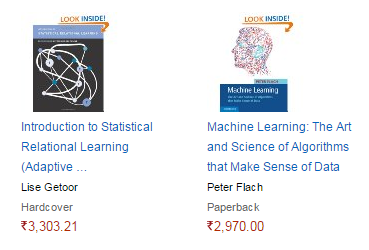
\includegraphics[width=0.4\textwidth]{Figures/amazon_reco}
%	\caption[Screen-shot of the Amazon book recommendation system.]{Books recommended by amazon.in while viewing the book "Predicting Structured Data" by Gokhan Bakir. It is desirable for the vendor to advertise related products in it's catalog.}
%	\label{fig:amazon}
%	\end{figure}


Learning algorithms have been applied to solve a variety of problems including, text or document classification, e.g. spam detection, subject identification, natural language processing, e.g. speech to text, part of speech tagging, computer vision, e.g. image classification, object identification, unassisted vehicle control, e.g. robot navigation, driver aids, optical character recognition (OCR), fraud detection (credit cards, telephones), network security e.g. intrusion detection, denial of service attack prevention, computational biology, e.g. protein function prediction medical diagnosis, recommender systems, e.g. search engines, related content identification, clustering systems, e.g. news collation, related tag identification;




This list is by no means exhaustive, and every day, learning algorithms are being used in new applications every day. It is possible to identify a number of broad templates to address like natured problems. Typical tasks for learning machines can be identified as,~\cite[7-10]{smolaML}
\begin{itemize}
\item \textbf{Binary Classification} involves the separation of input data into two classes. For instance, the example shown in Figure~\ref{fig:binclass}. In other words, given a pattern $x$ drawn from a domain $\chi$, the task is to estimate the value of an associated binary random variable $y \in {\pm1}$. The final decision may be depended on the input pattern, or on the sequence of input patterns. 

	\begin{figure}
	\centering
	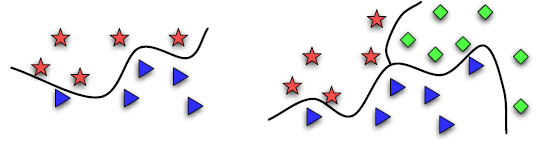
\includegraphics[width=0.7\textwidth]{Figures/classification}
	\caption[Illustration of classification.]{Binary classification (left); separate the stars from triangles. In this example it is possible to do so by drawing a straight line. This serves as an example of a \emph{linear classifier}. Multiclass Classification (right): 3-class classification is shown. Note that in the
	latter case we have a greater degree for ambiguity. For instance, being able to
	distinguish stars from diamonds may not suffice to identify either of them correctly,
	since we also need to distinguish both of them from triangles.}
	\label{fig:binclass}
	\end{figure}	

\item \textbf{Multi-Class Classification} is an extension of the binary classification problem, where the set of lables may assume a larger set of values, i.e. $y \in {1,\ldots,n}$. For instance we may want to classify emails into categories (Work, Personal, Promotions, Subscriptions, \ldots) according to the contents and the sender's address.  See Figure~\ref{fig:binclass} for an example. 
\item \textbf{Structuted Estimation} is an evolution of the multi-class classification problem. It attempts to improve the multi-classification results based on a known structure. For example an ontology may be used while attempting to classify research papers or seasonal temperature information may be used to aid iceberg detection.
\item \textbf{Regression} aims to estimate a real-valued variable $y\in\mathbb{R}$ given an input pattern $x$ (see Figure~\ref{fig:regs}). For instance, we might want to estimate the adrenaline level in a patient based on a blood cortisol measurement.

	\begin{figure}
	\centering
	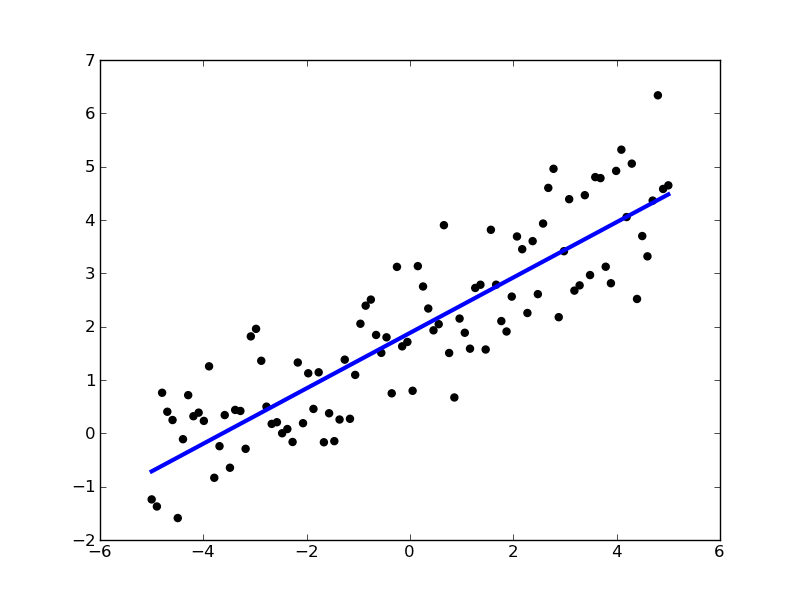
\includegraphics[width=0.5\textwidth]{Figures/regression}
	\caption[Illustration of regression.]{We are given a number of instances (indicated by the dots) and would like to find some function $f$ mapping the observations such that $f(x)$ is close to the input values.}
	\label{fig:regs}
	\end{figure}

\item \textbf{Ranking} is the task of using related parameters to order a set according to some predefined criterion. Internet search rankings are a common example of such a problem where we must rank and sort web pages according to their relevance to the search terms. 
\item \textbf{Clustering} involves the partitioning of input patters into homogeneous groups. For instance, using social media data to group people according to their interests.
\item \textbf{Dimensionality reduction or Manifold learning} involves the transformation of a representation of data into a lower dimensional representation with minimal loss of information. Hyper-spectral images have very high dimensionality (several hundred bands) which can be difficult to work with for computer vision tasks. By discarding irrelevant and redundant information, the dimensionality can be lowered.  
\end{itemize}

\section{The Problem of Representation}

	\begin{figure}
	\centering
	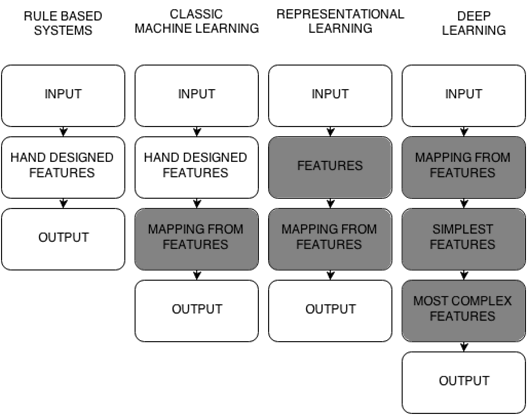
\includegraphics[width=0.7\textwidth]{Figures/deeplearning}
	\caption[Evolution of machine learning.]{Rule based systems are constructed to follow certain hand designed features and generalize poorly when unseen examples are presented. Classical machine learning attempts to learn a mapping from hand designed features, this gives it its generalization ability, however the task of designing the features itself is tedious. Representational learning aims to learn the features from the presented data, however this problem can become as difficult as the original problem itself. The shaded boxes represent the components that are able to learn from data. }
	\label{fig:deep}
	\end{figure}
	
Input data to a machine learning system can be represented in many ways, but some representations help improve the ability of a machine learning algorithm to extract knowledge from the supplied data. For example, numbers represented in the familiar binary notation may not always be successful in machine learning applications, and a one-hot representation may be preferred. The one hot notation involves setting successive bits high for successive numbers. For example, 1 is represented as $“0001”$, 2 as $“0010”$, 3 as $“0100”$ and so on. In a traditional binary representation, numbers that are in proximity to one another have very little similarity, for example 7 $(0000 0111)$ and 8 $(0000 1000)$ are separated by just one position on the number line, yet have no bits in common, while 64 $(0100 0000)$ and 1 $(0000 0001)$, which are quite far apart are separated by just one bit in the representation. This causes the learning machine to generalize poorly and will affect the performance of the architecture~\cite{Bengio-et-al-2014-Book}.

A lot of applications of machine learning involve input data that cannot be directly represented numerically. Computer vision for instance deals with images, the classification of spam email deals with raw text written in human languages. It becomes important to convert this input to a system that can be numerically encoded for input to the learning machine. The chosen parameters, which are used to represent a certain property of the data, are called features. The operation thus is a transformation of the data into the feature space. For instance, in an image corner points, lines and edges may be considered to be featured. In voice recognition, the pitch of the audio sample can be considered to be a feature.

Representation of the data is thus a central problem in the design of any machine learning algorithm. For many real-world applications, the selection of an appropriate representation scheme can be dauntingly difficult. One solution is to use a machine learning technique itself to capture not just the mapping from input to output but also the representation. This technique is called \emph{representational learning}~\cite{bengio2013representation}.

Learned features can offer a higher performance, and save human time and effort that would have been spent in constructing a hand designed model. However, identification of the features is not a trivial task.
\emph{Factors of variation} are used to examine the relation between the input data and the data. These factors may not be directly present or sensed in the data, but rather exist in the human mind that allows us to discriminate and make inferences about the data. These may be concepts and abstractions that help us process and understand the data.  


In the real world, every data sample is affected by a wide variety of factors, and it becomes important to separate these factors from the data, for instance, a tennis ball may become discolored over the course of a match, and the shape of the ball itself changes on impact. In this situation obtaining a representation of the data requires a human-like understanding of the data. In this situation, representational learning may not be helpful because the complexity of obtaining the representation is comparable to the solution of the original problem in itself.

	\begin{figure}
	\centering
	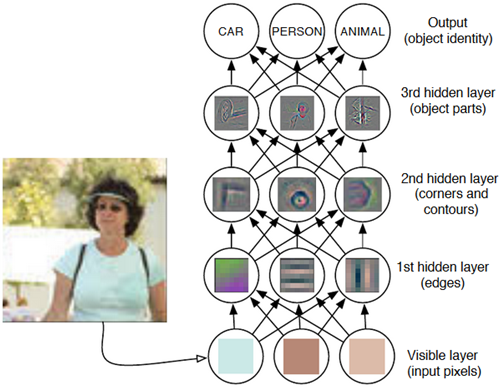
\includegraphics[width=0.6\textwidth]{Figures/deeplearning2}
	\caption[Illustration of deep algorithms.]{Deep learning algorithms attempt to represent the problem as a series of simpler sub-tasks. In the example shown, the task of recognizing the object in the image, is broken down into tasks of recognizing the edges in the image, then the corners in the next layer, then finally object parts in the third layer, which eventually leads to the identification of the object.  Image courtesy Zeiler and Fergus, Springer~\cite{zeiler2014visualizing}.  }
	\label{fig:deepimg}
	\end{figure}

\section{Deep Learning}

	\begin{figure}
	\centering
	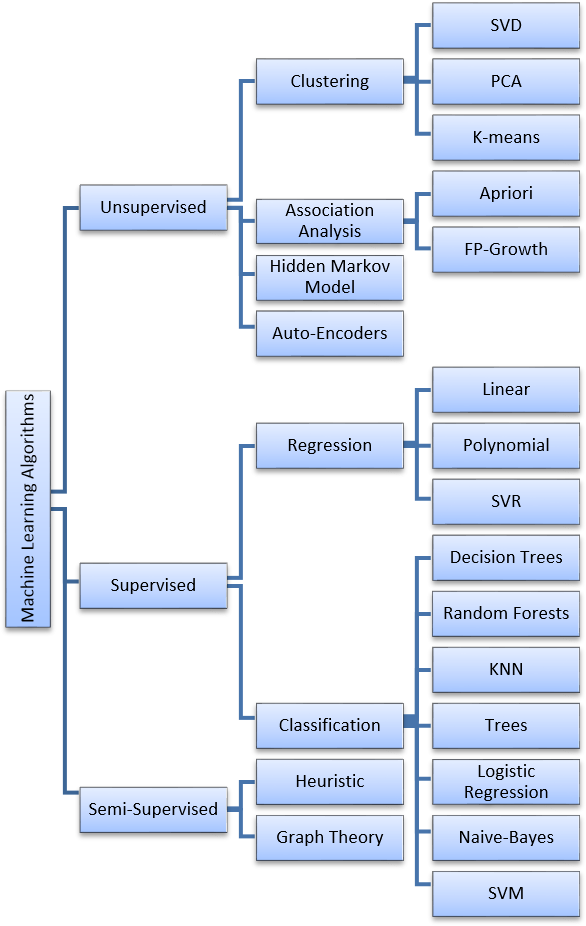
\includegraphics[width=0.7\textwidth]{Figures/MLtypes}
	\caption{Broad classification of machine learning algorithms by the nature of their training.}
	\label{fig:mltypes}
	\end{figure}

It can be difficult to learn high-level features from data. Deep Learning attempts to solve this by representing the original problem in a series of simpler sub-representations. The depth of the architecture refers to the number of levels of a composition of non-linear operations in the function learned. It allows the learning algorithm to learn a complex abstract concept from a series of more straightforward concepts. The multiple levels of abstraction will enable a system to learn complex functions mapping the input to the output directly from data, without depending on features crafted explicitly. At each level, features can be added to the representation. Thus it is not necessary to deal with all the features at once, like in shallow learning, allowing a more efficient way of dealing with a more complex representation. Deep learning breaks down the learning of the features into a pipeline where first simpler features are learned, which lead to the processing of increasingly complex features. 



In Figure~\ref{fig:deepimg} the task of object recognition is represented with a deep learning approach. At the first layer, we have the input pixels. This visual information is immediately recognizable to the human vision system, but is of little use to a leaning machine and is too complicated to map the object identity from a set of pixels. Learning at this stage is nearly impossible. We now break this complicated task into simpler sub-tasks, each dealing with a different layer of the representation. 
\begin{itemize*}
\item The first layer of the learning machine looks for the edges in the image by comparing pixel values of individual pixels with that of their neighbors. 
\item Once the edges have been represented, the next layer can represent the contours and corners as a set of edges. 
\item This, in turn, allows the third layer to group together these features to begin to identify object parts. 
\item Finally the output later can relate the parts to identify the object.
\end{itemize*}  

%\section{Recent advances in remote sensing}
%Despite the availability of 


\section{Classification of Remotely Sensed Images}
Classification of remote sensing images involves the grouping of pixels a scene or dataset into homogeneous groups, usually representing land cover classes or "themes". This categorized data can then be used to produce thematic maps of the areas represented in the image. Generally this is used to map distinct land-covers types like agriculture, urban and built up, forested, desert areas etc. The selection of the covers classes are application dependent, however certain standardized classification systems like the National Land Cover Data (NLCD) have been used operationally. The NLCD is a 21-class land cover classification scheme applied developed by the USGS Land Cover Institute for use in conjunction with Landsat Thematic Mapper data~\cite{jin2013comprehensive}. 

Usually multi-spectral data, like that from the Landsat mission, is used to perform classification.  The spectral pattern present for each pixel is used to discriminate the classes~\cite{lillesand1979remote}. These datasets allow for fairly accurate classification of large areas of the Earth's surface.  Data from the advanced very-high-resolution radiometer sensor (AVRIS) sensor aboard National Oceanic and Atmospheric Administration's (NOAA)  operational series of meteorological satellites was used by~\cite{Tucker25011985} to classify land-cover types and monitor changes in vegetation over the continent of Africa. At larger scales,~\cite{de1998global} generated a global land-cover classification dataset at a spatial resolution of 8-km using space-borne multi-spectral imagining systems and a decision tree classifier. A higher resolution dataset was derived from the Moderate Resolution Imaging Spectroradiometer (MODIS) sensor on-board Terra by~\cite{friedl2002global}. They generated a global land-cover map with a spatial resolution of 1-Km and using primarily the International Geo-sphere-Biosphere Programme Data and Information System (IGBP-DIS) classification scheme~\cite{Loveland97IGBP}.

Data from several medium resolution multi-spectral sensors like AVRIS, MODIS and Landsat TM have been used successfully for such applications due to their continuous global coverage, data availability and high spectral information content. However these sensors do have certain restrictions. They can not image during the night as they are dependent on the incident solar radiation for imaging. Cloud cover can also affect the quality of images as these sensors are unable to image though clouds. This is especially more of a problem while imaging areas covered with snow, as it can become difficult to differentiate the white snow covered land area from the white clouds. 

To overcome these problems, increasingly Synthetic Aperture Radar (SAR) data is being used for thematic map generation, especially over the cryosphere~\cite{jezek1998radarsat}. Certain applications also places temporal restrictions on the generation of thematic maps. For example, to generate ice-breg warning maps, the data can be acquired in a limited window and rapid and timely updates of these maps becomes critical~\cite{skvarca1994changes}. In such cases, it is also desirable to be able to produce these maps, operationally with a high degree of automation. 

Polarimetric SAR (PolSAR) imaging is an advancement made on single polarization SAR imaging. The polarization of the incident wave is controlled so that it is restricted alternatively to either H or V transmission. Similarly, reception is performed alternativly in H or V polarizations, so that for every imaged pixel, four combinations of polarization i.e. HH, HV, VH and VV are captured. PolSAR imaging can capture more information about the physical properties of the target than possible with single or dual polarization imaging, and consequently, this can lead to better classification~\cite{Lee2001multipolclass}. 

	\begin{figure}[tbp]
	\centering
	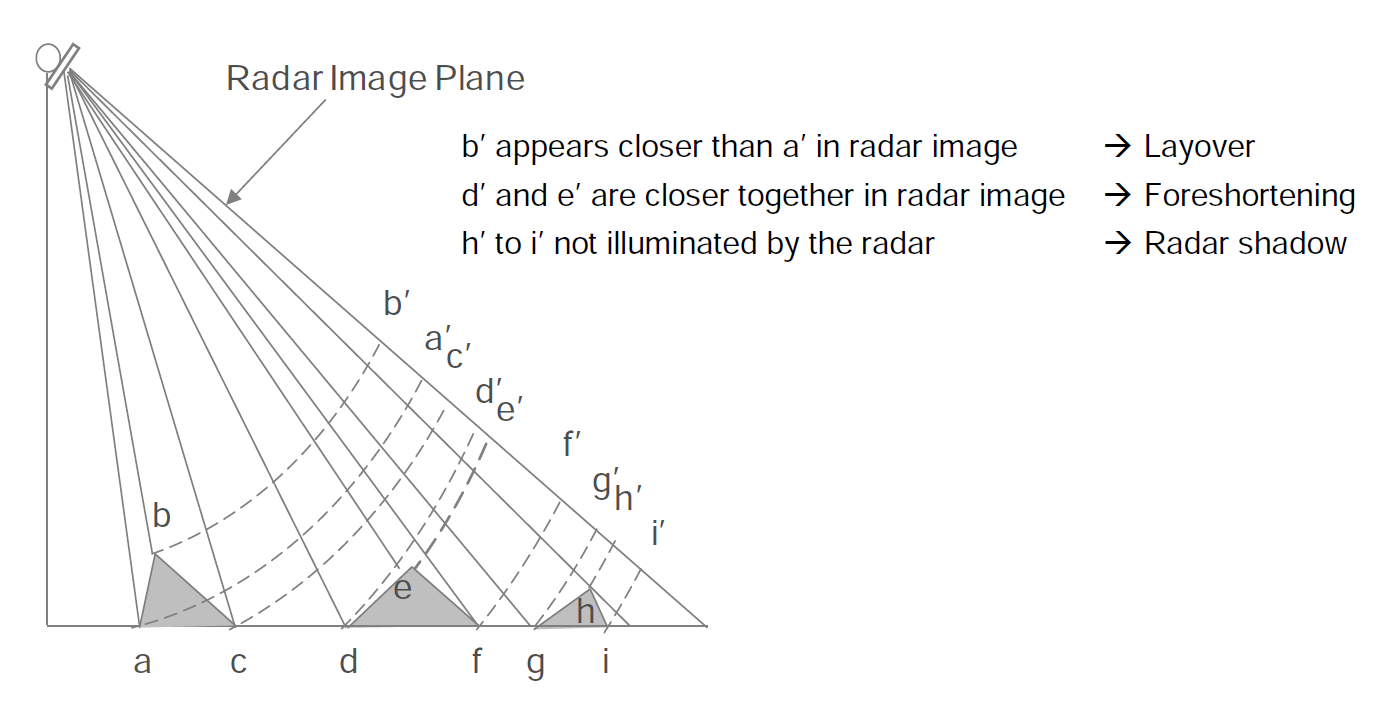
\includegraphics[width=\textwidth]{Figures/geometricSAR}
	\caption{Geometric distortions in SAR imaging due to the side looking geometry.  Image courtesy VanZyl, Wiley~\cite{van2011synthetic}.  }
	\label{fig:sargeo}
	\end{figure}
	

\section{Challenges in SAR Image Classification}

SAR imaging introduces its own set of challenges to the classification problem. Being an active sensor, it must supply the illuminating energy, i.e. radar pulses, which necessitates that a power source be tethered to the sensor. Satellite sensors are usually powered by a battery which is rechargeable by solar energy. This limits the sensors continuous operation capability. Unlike optical sensors, which can be operated continuously, a typical modern spaceborne SAR sensor can only be operated for ~11 minutes per ~90 minute orbit~\cite{simpson2004terrasar}. This makes it difficult to generate the updated global mosaics that are generated using multi-spectral sensors~\cite{stockli2005blue}. Additional, in PolSAR mode, because each pixel is imaged twice on two subsequent pulses, the effective swath width of the imaged strip is half as compared to a single polarization SAR system. This somewhat reduces the feasibility of PolSAR in generating thematic maps of large areas. 

	\begin{figure}[tbp]
	\centering
	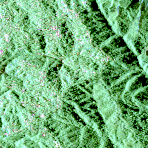
\includegraphics[width=0.4\textwidth]{Figures/shadow}
	\caption{Crop of a Pauli RGB image generated from a UAVSAR dataset showing layover (bright) and shadow (dark) areas.  }
	\label{fig:sarshadow}
	\end{figure}
	


Unlike optical images, which are acquired with the sensor facing towards the nadir, SAR images are acquired in side look geometry~\cite{lee2009polarimetric}. RADAR images are formed by fundamentally from the echoes returned from targets, thus a RADAR that faces vertically down would not be able to distinguish echos from equidistant targets that lie on either side of the sensor. In non imaging radars with a narrow beam-width, like sounders, this behavior is desirable, but it makes imaging impossible. The side looking geometry introduces geometric artifacts like layover, foreshadow and shadow effects. This causes elevations in the imaged terrain (buildings, hills and mountains) to suffer from certain distortions in the produced image~\cite[21]{van2011synthetic} as shown in~\ref{fig:sargeo}. Along with the shape distortion, foreshortening also manifests as an area of bright RADAR return, which can cause the land-cover type in these areas to mis-classified. Similarly, shadow regions appear dark in the image and contain no echo information, making classification difficult as shown in Figure~\ref{fig:sarshadow}

\begin{figure}
\label{fig:statistics}
 \centering
        \begin{subfigure}[b]{0.65\textwidth}
                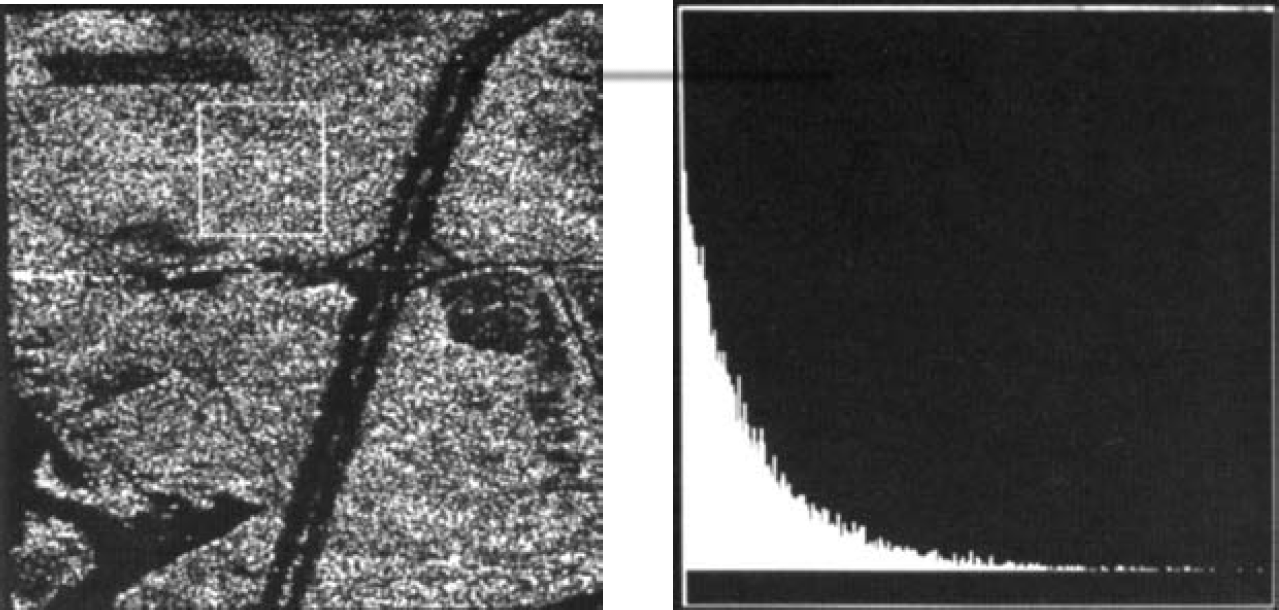
\includegraphics[width=\textwidth]{Figures/lee1}
                \caption{}
                \label{fig:stat1}
        \end{subfigure}%
        \hspace{0.1em}
        \begin{subfigure}[b]{0.65\textwidth}
                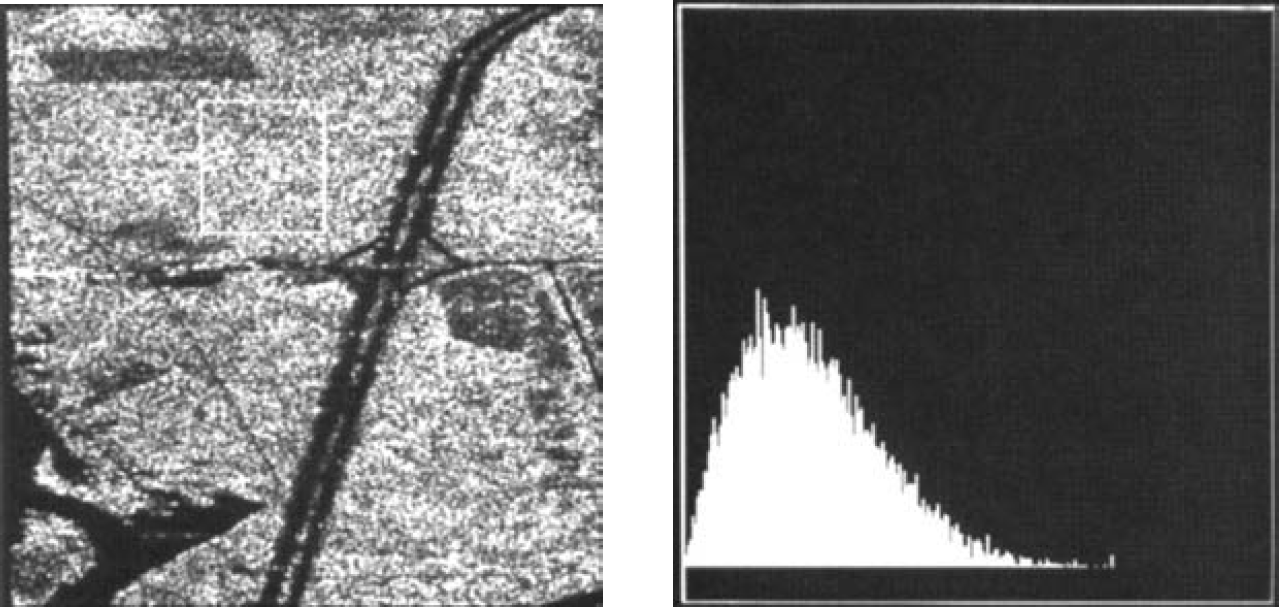
\includegraphics[width=\textwidth]{Figures/lee2}
                \caption{}
                \label{fig:stat2}
        \end{subfigure}%
        \hspace{0.1em}
        \begin{subfigure}[b]{0.65\textwidth}
                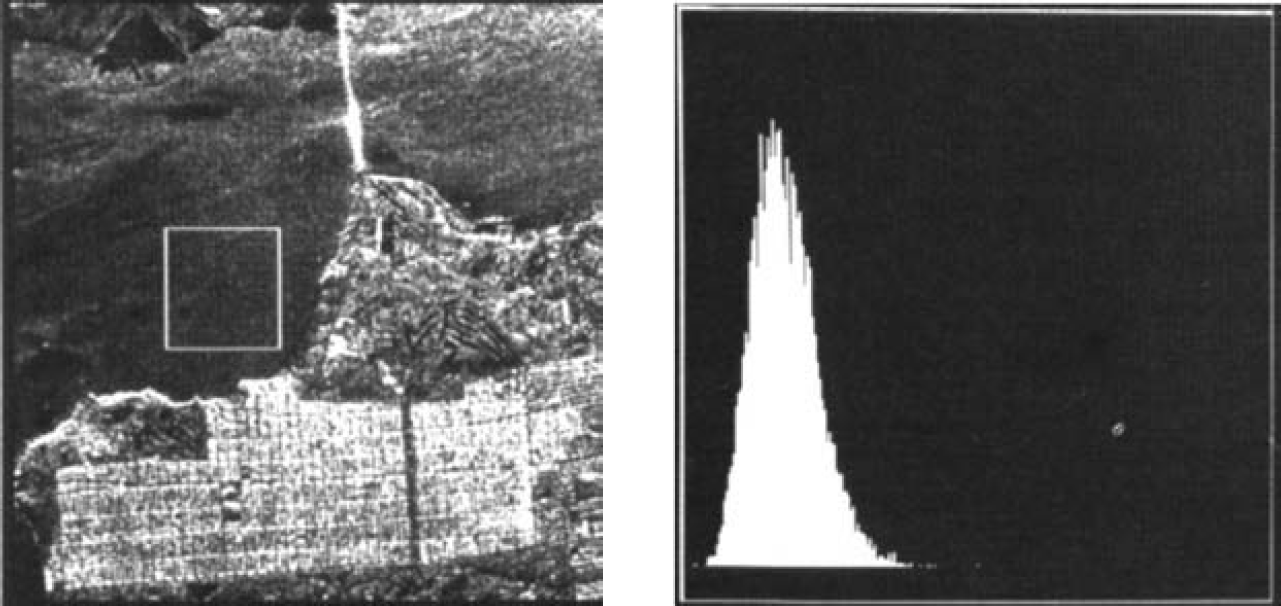
\includegraphics[width=\textwidth]{Figures/lee3}
                \caption{}
                \label{fig:stat3}
        \end{subfigure}%

             
\caption[SAR speckle statistics]{ SAR speckle distribution are plotted for intensity and amplitude images of different looks. (~\ref{fig:stat1})  1 Look intensity SAR image with it's histogram (exponential distribution). (~\ref{fig:stat2})  1 Look amplitude SAR image (same area as before) with it's histogram (Rayleigh distribution)   
(~\ref{fig:stat3})  4 Look amplitude SAR image with it's histogram (chi distribution).
Figure courtesy Lee and Pottier~\cite[104]{lee2009polarimetric} }
\end{figure}

Apart from the problems related to the physical constraints of the images, like other coherent imaging techniques, suffers from the problem of speckle~\cite{gagnon1997speckle}. Speckle noise can complicate the task of classification of SAR images. Further, the speckle pattern is non often non-Gaussian in distribution, thus filtering and classification techniques that have been developed for Gaussian optical images can not be directly applied to SAR images. Various non Gaussian models have been proposed to represent SAR data~\cite{jakeman1976model}. To represent PolSAR data multivariate K distribution based models have been proposed~\cite{lee1994k}, ~\cite{doulgeris2010scale}. This was further extended by~\cite{freitas2005polarimetric} who used the G distribution to model the speckle pattern. Non Gaussian model based classification techniques have been applied by~\cite{akbari2010non} to segregate glacier ice types to track changes in the glacier.  Various statistical parameters which can be exploited in conjecture with machine learning techniques to alleviate some of the challenges of the classification of PolSAR images.

\section{Generative and Discriminative Classifiers}
Generative classifiers learn a model of the joint probability, $p(x|y)$, where $x$ represents the inputs and $y$, the labels. They make their predictions according to the $p(x|y)$ computed using the Bayes rule and then selecting the label $y$ with the highest probability. Discriminative classifiers model the posterior $p(y|x)$ directly or learn from a direct map from inputs $x$ to class labels. It is more attractive to use discriminative classifiers are over generative ones. According to~\cite{vapnik1998statistical}, the classification problem should be solved directly and not as an intermediate step such as modeling of the probability $p(X|y)$. An experimental comparison of this can be found in~\cite{ng2002discriminative}.

 % OK


\section{Supervised Urban Classification}    
%%%%%%%%%%%%%%%%%%%%%%%%%%%%%%%%%%%%%%%%%%%%%%%%%%%%%%%%%%%%%%%%%%%%%%%%%%%%%%%%%%%%
%%%%%%%%%%%%%%%%%%%%%%%%%%%%%%%%%%%%%%%%%%%%%%%%%%%%%%%%%%%%%%%%%%%%%%%%%%%%%%%%%%%%
%% Urban classification - Trento_2015 - 2_method.tex




%\title{Deep Learning for Urban Classification}
%\date{}
%\author{SD, LB, AB, FB, SC}
%\maketitle

%\section{Introduction}

Remotely sensed images acquired by space- or airborne sensors have revolutionized Earth observation allowing an unprecedented ability to image and observe large areas with high temporal repetivity. 
This has opened new avenues for the monitoring of dynamic Earth processes. Long-term Earth observation missions have ensured data continuity allowing the characterization of anthropocentric processes and changes. Spaceborne optical sensors can deliver continuous global coverage, data availability, and high spectral information content. However, these sensors can not image during the night or inclement weather as they are dependent on the incident solar radiation for imaging. 

The active properties of Synthetic Aperture Radar (SAR) data are increasingly exploited in monitoring applications. SAR sensors form an image by transmitting radar pulses  either in horizontal or vertical polarization and receiving coherently ~\cite{curlander1991synthetic}.  These sensors are not dependent on external sources for illumination. They have cloud cover penetrating capabilities thus operate without restriction of time and season.  Polarimetric SAR (PolSAR) imaging is an advancement made on single polarization SAR imaging~\cite{van1992nasa}. The polarization of the incident wave is controlled so that it is restricted alternatively to either $h$ or $v$ transmission. Similarly, reception is performed alternatively in $h$ or $v$ polarizations, so that for every imaged pixel, four combinations of polarization (i.e. $hh$, $hv$, $vh$, and $vv$) are captured. PolSAR imaging can capture more information about the physical properties of the target than single or dual polarization imaging, and consequently, it can lead to better target characterization and classification~\cite{Lee2001multipolclass}. However, it introduces unique challenges in the characterization of urban areas, which is increasingly becoming important for systematic monitoring.

%Why urban classification - climate change
% % % % % % % % % % % % % % % % % % % % % % % % % % % %
In the past decades, there has been a rapid inflation of population and the consequent expansion of urban areas. A high concentration of human population lives in urban areas, and it becomes important to monitor the growth and expansion of these regions. In the case of natural calamities like floods, earthquakes, and tsunamis, it is important to derive information at the earliest to guide mitigation actions. In such cases, the availability of up-to-date  classification maps of urban areas, which can be referenced against post-event data, is crucial. The accurate classification of urban areas is the first step towards operational implementation of these applications.
For tropical regions, many high population urban centers are shrouded by cloud cover for months at a time during the monsoon season. During this time, these areas are also the most susceptible to flooding.  Due to the dense cloud cover, it becomes difficult to perform routine monitoring operations during this period using optical sensors. However, radar data are relatively unaffected by weather phenomena and can image on-demand irrespectively of conditions or illumination providing crucial information in these scenarios. 
% % % % % % % % % % % % % % % % % % % % % % % % % % % % % % %



%challenges - not direct
% % % % % % % % % % % % % % % % % % % % % % % % % % % % % % % % % % % %
SAR imaging introduces its own set of challenges to the classification problem. SAR images are acquired in side look geometry, which introduces geometric artifacts like the layover, foreshadow and shadow effects. This causes elevations in the imaged terrain (buildings, hills, and mountains) to suffer from certain distortions in the produced image making classification difficult. Moreover, SAR being a coherent imaging technique, suffers from the problem of speckle which further complicates the task of classification of SAR images. The speckle pattern is often non-Gaussian in distribution~\cite{jakeman1976model} making its suppression nontrivial. 
% challenges direct goes here
% % % % % % % % % % % % % % % % % % % % % % % % % % % % % % % % % % % % %

Thus filtering and classification techniques that have been developed for Gaussian optical images cannot be directly applied to SAR images. Various non-Gaussian models have been proposed to represent SAR data~\cite{jakeman1976model}. To represent PolSAR data multivariate K distribution based models have been proposed~\cite{lee1994k}, ~\cite{doulgeris2010scale}. This was further extended by~\cite{freitas2005polarimetric} who used the $G^0$ distribution to model the speckle pattern. Non-Gaussian model-based classification techniques have been applied by~\cite{akbari2010non} to segregate glacier ice types to track changes in the glacier.  


%LR
The first attempt at the classification of PolSAR images was made in~\cite{kong1988identification}. The authors proposed a maximum likelihood-based classification method for a PolSAR image based on a complex Gaussian distribution and showed that the addition of phase information from multiple channels improves the classification accuracy. Subsequently, a neural network classifier for SAR data was proposed in~\cite{pottier1991radar}, where a feed-forward network with a single hidden layer having sigmoidal activation functions was showed. It was observed that polarimetric and machine learning theory were complementary. However, at that time neural networks were considered computationally intensive and would not be widely adopted until subsequent advancements in computing technology~\cite{anderson1995introduction} were made.

A popular classification scheme was proposed in~\cite{lee1994classification}, which uses a maximum likelihood classifier based on the Wishart distribution to perform terrain classification. Various studies have explored the effect of speckle and sensing frequency on the accuracy of this technique~\cite{lee2001quantitative}. An unsupervised scheme also based on the Wishart distribution was proposed in~\cite{lee2004unsupervised}. This has been extended by using several techniques for urban classification. In~\cite{dabboor2013unsupervised} the Chernoff  and in~\cite{dabboor2014jeffries} the Jeffries-Matsushita distance measures are used in conjunction with the complex Wishart distribution. 
The complex Wishart distribution model for the covariance or coherency matrices is valid for homogeneous areas. %Textured areas are modeled by a Gamma distribution instead.  
%For heterogeneous or
However, in extremely heterogeneous regions, like urban areas, the Wishart assumption    is seldom true. Hence, in this case, it is desirable to use a non-parametric classification scheme. 
%The proposed method does not make assumptions about the prior distribution of the data.


Polarimetric scattering power decomposition parameters can serve as low-level features in classification~\cite{bhattacharya2015adaptive}. In~\cite{bhattacharya2012polarimetric} information theory is used to select a subset of the Touzi scattering decomposition parameters, which are then classified using a Support Vector Machine. A multi-decomposition parameter approach was adopted in~\cite{niu2013multi}, which used an SVM and a rule-based approach to urban land-cover classification. 
Both supervised~\cite{da2008land} and unsupervised~\cite{lee2004unsupervised} schemes have been proposed that perform urban area segmentation based on decomposition parameters. 
Despite the availability of several sophisticated methods, the selection of an appropriate decomposition approach for a scene is not a trivial task~\cite{chen2014modeling}. An alternative strategy for urban classification is to use the textural information  in the SAR images~\cite{1344157, 1183703}. However, in texture based schemes, the rich scattering information available from polarimetry is often not considered. 
In the classification of urban structures is performed by using the Fisher distribution with Markovian segmentation for identification of ground, buildings, and vegetation. Other texture based schemes have also proved useful for urban segmentation~\cite{1183703}. 

Interest in neural networks was renewed with improvement in technology. In~\cite{214928} a Karhunen-Loeve transform is used to extract features from a fully polarimetric dataset and a neural network is used to perform classification of the scene into urban, vegetation and terrain classes.   A study about the land-cover and soil type mapping capabilities using a probabilistic neural network was reported in~\cite{antropov2014land}  using L-Band space-borne data. Multi-temporal/multi-frequency datasets were exploited using a neural-statistical kernel in~\cite{1237401} for urban classification. An adaptive resonance theory neural network   was shown to perform computationally efficient classification of urban areas using polarimetric data. Hybrid approaches such as a combination of neural networks and fuzzy logic were demonstrated to have good performance for SAR classification in~\cite{655339} and later specifically for identification of urban areas in~\cite{gamba2003increased}. A system for classification of multitemporal SAR images based on the integration of the SAR system physics and a radial basis function neural network architecture is proposed in ~\cite{4623140}. Another multi-temporal approach using single-channel SAR datasets to monitor urban land cover in major Italian cities is proposed in~\cite{doi:10.1080/01431160118746}. 

Hinton et. al. introduced the concept of deep learning in ~\cite{hinton2006fast}, which found successful application in multiple areas~\cite{he2015delving, deng2013recent, glorot2011domain, mnih2013playing} establishing it as a new field of machine learning research. 
The motivation lies in the capability of neural networks to break down complex learning problems into simpler representations. Deep Learning has been recently adopted by the remote sensing community for improved performance in several applications~\cite{han2015object,tang2015compressed,chen2014vehicle}. Multiple natural land cover classes were identified from a hyperspectral dataset in~\cite{chen2014deep}, while objects detection was performed in optical datasets in~\cite{han2015object} using deep learning techniques. Additional information is often added to the classification scheme from auxiliary data sources like optical and multi-spectral areas~\cite{zhu2012assessment,6202721}. Deep learning techniques are quickly gaining popularity to perform multi-sensor data fusion as well~\cite{zhang2015deep,li2008remote}. A deep learning based approach can simplify feature and classifier design, and allow the utilization of augmented datasets. This can help mitigate some of the challenges faced in the classification of urban areas from PolSAR data.  



%In this work we adopt a deep learning based architecture to overcome certain challenges faced in the classification of urban areas from polarimetric SAR data.


%pixel based classification ka para
%Pixel based classification is a common methodology adopted in the remote sensing community. Various approaches such as handcrafted features~\cite{benediktsson2005classification, zhang2006pixel, huang2012morphological}, discriminative feature learning~\cite{jia2013feature, zhang2012combining} and sophisticated classifier design~\cite{melgani2004classification} have been demonstrated in literature. A deep learning based approach can simplify feature and classifier design while achieving good performance.
 
The classification of urban areas in PolSAR data-sets is especially challenging, because of the problems related to the orientation of targets with respect to the radar line of sight.
When targets that exhibit even bounce scattering are oriented away from the radar line of sight, the co-polarized return is reflected away from the sensor, while the cross-polarized return level remains the same~\cite{yamaguchi2011_y4r,7862796}. This makes such areas hard to distinguish from natural targets like forest and vegetation. This represents a major challenge for the classification algorithm. In~\cite{chen2014uniform} a polarimetric matrix rotation theory framework was proposed which develops a physically significant set of rotation angle parameters.  An approach based on the rotation of the coherency matrix was proposed in~\cite{yamaguchi2011four} to compensate for the over-estimation of volume in rotated urban areas. In~\cite{zou2016eigen}   a link is established between eigen-decomposition method and model-based decomposition methods to also solve the overestimation of the volume scattering power problem. Another decomposition technique proposed in~\cite{7872383} uses a mapping to create an improved representation and further help improve target characterization. 

% % % % % % % % % % % % % % % % % % % % % % % % % % % % % % % % % %
Various statistical parameters and understanding of the physics of scattering can be exploited in conjecture with appropriate machine learning techniques to alleviate some of these difficulties. In addition to the challenges of the sensing medium itself, the data volumes that will potentially be generated from current and future SAR programs, viz. NISAR and Sentinel, pose  additional predicaments. These missions are being designed with systematic global coverage capability that will lead to generation of a spatially and temporally dense collection of data. While this can lead to better understanding of of the Earth, leveraging this information is an additional challenge. Manual analysis of this kind of data-sets are infeasible and automated of semi-automated machine learning techniques which have a relatively low computation time are instrumental in extracting relevant information. 
% % % % % % % % % % % % % % % % % % % % % % % % % % % % % % % % % % %

%motivation
%Current classification algorithms documented in literature do not fully %leverage the physics of the polarimetric scattering phenomenon. 
%As a result of this the classification accuracy of these techniques in %areas with targets rotated with respect to the radar line of sight is %limited. 
Alternatively, some approaches utilize a separate class for identifying rotated targets and then merge them with the non-rotated class as a post-classification step.  However, this makes it mandatory to input training samples from rotated target areas, which may not always be possible. The generalization ability and autonomy of such an approach is therefore low.

This might not always be available for a given scene and changes if the flight line of the platform is varied. The generalization ability and autonomy of such an approach is therefore low. 
Sophisticated models have been developed to account for the rotation problem. While such approaches produce accurate results, they are computationally intensive making them infeasible for high data volumes.  
In this work, a novel technique based on the target scattering properties along with a deep learning approach is proposed for urban area classification using PolSAR data. The properties of polarimetric scattering are used to generate synthetic targets, which simulate the effects of rotation about the radar line of sight in uniform angular steps.
In general, polarization orientation angle shifts are observed in polarimetric SAR data which are induced by terrain slopes and complex scattering in urban areas. In turn, polarization orientation angle shifts can be induced by appropriate Euler rotations to form synthetic targets. They can be suitably leveraged for better generalization in machine learning algorithms. The process is used to generate a database containing simulated urban targets. 
The synthetic urban target database is used to train and extract features from a  sparse stacked auto-encoder. Thus, the information about the targets and rotation is accounted for in the classification scheme, which helps to discriminate rotated urban areas without requiring explicit representation in the training stage. The advantage of using a deep learning based scheme is that the network can be trained incrementally on a large volume of data, and subsequently used as a generalization for unseen data. This leads to a computationally efficient and fast classification phase. Given the commercial interests in deep learning at large scale, several GPU based specialized peripherals have been developed. These can be used to further speed up calculations and drastically reduce the training time over CPU bound computation. 


%In this paper, the polarimetric SAR dataset is the low-level features.  Following this, a stacked auto-encoder is used to learn and extract high-level features in an unsupervised manner. Finally, a multi-layer perceptron is used to perform the final classification in a supervised manner.

% novelty
%In this work, we use a novel technique to overcome some challenges faced in urban area classification. We use the physical properties of the polarimetric data to generate synthetic targets which simulate the effects of rotation about the radar line of sight. This generated synthetic urban target database is used to extract features using the stacked auto-encoder. Thus, the information about the target and its rotation is accounted for in the classification scheme, which helps discriminate rotated urban areas, without having to exclusively specify these areas in the training stage. 

% % moved
%In this work, we propose and deep learning architecture and a technique based on the physics of scattering to overcome some challenges faced in urban area classification. 
%A physics-based target generation technique and a deep learning architecture for the pixel-based classification of polarimetric SAR data is presented. 

%%%%% PAPER SUMMARY: MAYBE COMMENT %%%%%%%%%%%%% >>>
%The urban synthetic target database generation technique applied to simulate the effects of rotation about the radar line of sight (Section~\ref{sec:stage1}).  This forms the mid-level features which then act as input to a stacked auto-encoder stage. The training of this stage is carefully monitored using metrics derived from information theory (viz. cross-entropy error) to prevent over-fitting. After the training phase, the extracted features are described and discussed in section~\ref{sec:stage2}. Finally, a multi-layer perceptron is used to perform the final supervised classification using both the extracted features and estimated statistical parameters (Section~\ref{sec:stage3}). The overall stage-wise procedure allows an efficient tuning of hyper-parameters for optimizing the classification. The technique is demonstrated on PolSAR data acquired over the city of San Francisco by the UAVSAR and ALOS-2 platforms (Section~\ref{sec:stage4}). It is shown that  both rotated and non-rotated urban areas can be discriminated with an overall accuracy of about $91.3\%$.  Moreover, the proposed approach shows a better qualitative and quantitative performance when compared with contemporary techniques.%~(Section~\ref{sec:results1}). 
%%%%% PAPER SUMMARY: MAYBE COMMENT %%%%%%%%%%%%% <<<

%moar menucard + expectation

%dataset?


                          

%%%%%%%%%%%%%%%%%%%%%%%%%%%%%%%%%%%%%%%%%%%%%%%%%%%%%%%%%%%%%%%%%%%%%%%%%%%%%%%%%%%%
%%%%%%%%%%%%%%%%%%%%%%%%%%%%%%%%%%%%%%%%%%%%%%%%%%%%%%%%%%%%%%%%%%%%%%%%%%%%%%%%%%%%
 % OK

%% CD methodology
\section{Semi-supervised Urban Change Detection} 
Urban Change Detection (CD) is an important part of monitoring operations and is done to study changes induced by urbanization or in response to natural disasters for relief operations.

The active imaging capabilities of a Synthetic Aperture Radar (SAR) system allows imaging in inclement weather and illumination conditions. This is highly desirable for urban mapping and change detection applications, especially in the tropical regions where the monsoons obscure urban centers from view of optical sensors for many months. It is also during this period that calamities like floods are most likely to occur making the rapid imaging ability of SAR sensors crucial. Polarimetric SAR (PolSAR) is an advancement over traditional SAR imaging that involves the simultaneous coherent transmission and reception of signals  vertically and horizontally polarized in quadrature. This allows a better characterization of the target being imaged leading to improved discrimination capabilities when compared to single polarization acquisitions~\cite{lee2004classification}. 

CD aims at identifying changes occurred on the ground between two or more acquisitions on the same geographical area at different time instants. The complexity of collecting ground reference samples makes unsupervised approaches the most relevant in the field. The unsupervised change detection procedure can be generalized to consist of three distinct steps: Image pre-processing, Change Index (CI) generation and subsequent thresholding of the CI. Pre-processing includes accurate registration of multi-temporal images which is critical for the accuracy of the technique as a whole. Significant progress has been made in this direction for SAR and sub-pixel registration accuracy is common~\cite{li2008image}. For SAR data log-ratio CI is the most commonly exploited~\cite{bazi2005unsupervised}. The CI is usually thresholded to form the final binary or multi-class map based on physical properties of the change index or its statistics~\cite{bruzzone2000automatic}.
%bazi2005unsupervised rignot1993change
%Although this is effective for characterizing the change, polarimetic information, and thus ability to perform classification or inversion, from the unchanged areas is lost due to the ratio operation. 
PolSAR data have not been  widely exploited for change detection applications, but with greater availability of data they are becoming increasingly important. A framework for joint analysis of the PolSAR features was explored for multiple change detection~\cite{pirrone2016novel}. Approaches based on PolSAR descriptors~\cite{6310048} and distribution test statistics~\cite{conradsen2003test} have also shown to be effective. 


%In this paper, a novel Deep Neural Networks (DNN) based framework is proposed leveraging the enhanced information content of multi-temporal PolSAR images.  
DNNs have previously been used  for single polarimetric SAR images~\cite{zhang2016deep} only. 
The proposed approach takes an input, a pair of PolSAR images and learns a representation that maximizes the separation of changed areas from  unchanged ones in the multi-temporal stacked feature vectors (manifold) domain. This representation is  exploited by a weakly supervised MLP technique to generate a change map. 
%Section~\ref{sec:Method} discusses the proposed methodology. The study area and dataset are described in Section~\ref{sec:exp} and results are reported in Section~\ref{sec:result}. % OK


%% Crop classification methodology
\section{Multi-frequency Crop Classification } 
PolSAR is an advanced imaging technique which coherently transmits and receives radar pulses in quadrature polarization. The multi-frequency polarized waves are susceptible to different structure, orientation and dielectric properties of the medium. Various PolSAR systems (viz. AIRSAR, EMISAR, and F-SAR) are capable of simultaneous multi-frequency full PolSAR data acquisition allowing for improved target characterization~\cite{499786}.  

%%%%%%%%%%%%%
% Early study
%%%%%%%%%%%%%


The use of single-frequency and single-polarization SAR data has limited success in land cover classification, even when temporal changes in the scattering are exploited, especially for agricultural applications~\cite{mcnairn2009contribution}.
Techniques like hierarchical segmentation \cite{liu2016hierarchical}  and sketch maps in conjunction with adaptive Markov random fields~\cite{Junfei2016} have demonstrated to obtain an accurate classification for single frequency PolSAR data by leveraging contextual information while preserving edges.
Early studies~\cite{baronti1995sar,ferrazzoli1997potential} have evaluated the effectiveness of multi-frequency PolSAR data acquisition for crop identification. Furthermore, an exhaustive comparison on the use of multi-frequency single, dual and fully 
polarimetric acquisition was performed in~\cite{lee2001quantitative}, with the assessment of quantitative classification accuracy. It was found that the integration of polarimetric information from multiple bands leads to an improved classification performance.  Different strategies have been adopted to combine information from multi-frequency observations. An early approach for multi-frequency PolSAR classification is described in~\cite{499786}. It uses a dynamic neural network to combine the information from C-, L- and P-bands for classification.
% %V3
In~\cite{fukuda1999wavelet}, a wavelet-based textural feature set is derived, which is subsequently classified by a minimum distance classifier. However, it is indicated that a more sophisticated neural network technique might have a better performance. 
%
Parameters derived from the decomposition of multi-temporal L-band PolSAR data combined with single polarization C-band data was used in~\cite{mcnairn2009contribution} for crop classification. 
An unsupervised classification technique using dual-frequency PolSAR datasets is introduced in~\cite{964969Famil2001}. 
A $6\times6$ polarimetric coherency matrix is constructed to combine the multi-frequency information. The methodology uses an iterative algorithm based on a complex Wishart density function to classify the multi-frequency data.
%
Although it is effective for two frequencies, it is challenging to extend this technique to combine three or more bands, since the statistical parameter estimation equations must be derived. 
%
%It is a classification with the Wishart classifier on a 6x6 coherency matrix after an initial segmentation in the $H/A/\alpha$ space assuming�that the coherency matrix in two frequencies is statistically dependent.�
In~\cite{hoekman2003new}, a matrix reversible transformation approach is developed to combine multi-frequency PolSAR datasets into a representation with a simplified statistical description for classification. However, the approach requires extensive \emph{a-priori} knowledge of the datasets leading to a redundant representation.
%%%%% V3
In PolSAR data analysis, the second order statistics (coherency and covariance) can be expressed as a Sum of Kronecker Products (SKP) of two matrices~\cite{tebaldini2009algebraic}. In this, one matrix accounts for the scattering mechanism, while the other characterizes its spatial structures. SKP has been explored for the integration of multi-baseline PolInSAR datasets.




The combination of multi-frequency information however causes a simultaneous increase in dimensionality of the feature set. In classical machine learning, an increase in dimensionality causes increased complexity for the learning technique. This is undesirable for efficient training which is usually referred to as the ``curse of dimensionality''~\cite{vapnik1998statistical}.  To this end, dimensionality reduction techniques like the principal component analysis, independent component analysis and non-negative matrix factorization are applied as a pre-processing step before training the learning algorithm which results in a loss of information. However, by exploiting techniques like the Deep Neural Network (DNN), it is possible to incorporate the information without the dimensionality reduction step~\cite{cichocki2015tensor}.  


The combination of multi-frequency information causes a simultaneous increase in the dimensionality of the feature set. A classification task is often easier to solve in a higher dimensional space. 
%
%In this paper, a novel tensorization framework utilizing the Kronecker product for the combination of multi-frequency PolSAR data, and its subsequent classification using an Artificial Neural Network (ANN) is proposed. The tensorization leads to increased dimensionality, which is exploited by an ANN architecture to achieve improved classification performance over simple augmentation of data from multi-frequency bands. 
%The ANN comprises of two stages where an unsupervised stochastic sampling Auto-Encoder (AE) learns an efficient representation and a supervised Feed Forward (FF) network performs classification.
%The proposed framework is demonstrated for multi-frequency classification of an agricultural and a forested scene.
%
%The framework can be further extended for multi-temporal and multi-incidence datasets.
Upcoming space-borne missions like~\cite{rosen2015nasa} are planned to have multi-frequency systematic PolSAR data collection capabilities, making it important to develop frameworks capable of leveraging the data. % OK

\section{Snow-Cover Classification}
Snow cover variation is a sensitive indicator of environmental change. Therefore, snow cover mapping is a critical exercise which is supposed to be performed at regular intervals. Observations at periodic intervals require a sensor independent of time and weather. Microwave remote sensing is a reliable tool for the timely observation of spatial and temporal variability of snow-pack characteristics. 

Approaches like~\cite{slater1999potential} proposed multi-sensor constellations for quantifying snow-cover, especially in the sub-polar maritime regions. They highlighted the problems faced in mapping the ephemeral nature of snow in such regions, in light of lack of access to imagery on occasion due to cloud cover. Although, a multi-sensor approach can be sufficient for snow-mapping, it is usually economically infeasible to cover continent scale areas, if the data is to be purchased. Microwave based approaches, which are unperturbed by the presence of cloud cover, are more practical and efficient for the task. In~\cite{grody1991classification} a seven-channel microwave radiometer was demonstrated for snow-cover mapping. Such a passive sensor is able to operate continuously, and with its large footprint, is able to cover large areas of the Earth's surface. At the same time, due to the nature of microwave radiation it is not affected by cloud cover. However, the disadvantage is that the resolution is coarse. Active SAR sensors have a much higher spatial resolution, while also being unaffected by cloud cover~\cite{shi1994snow}. Although active sensors have a smaller coverage than passive ones, they have far increased ability to mapped details. SAR is a side-looking imaging technique, which leads to geometric distortions like layover and shadow. These artifacts can be mitigated by using a hybrid approaches that merges optical and SAR data~\cite{koskinen1999snow}.
%
Advanced SAR techniques like InSAR have been explored to improve classification performance, especially in challenging conditions like wet snow. In~\cite{strozzi1999mapping} the degree of coherence was used to delineate wet-snow, in areas where backscatter alone was insufficient. PolSAR techniques can also be used to recover information in such conditions. In~\cite{surendar2013improved} an advanced technique to estimate snow wetness has been described, which can be extended to improve the accuracy of snow-cover classification maps.

The capabilities assessment of several polarimetric parameters including a supervised classification technique to discriminate snow-covered areas was carried out over the Indian Himalayan region~\cite{singh2014capability}. The proposed polarization fraction ($PF$) scheme for wet snow mapping, in the absence of any training samples, performed better than the rest of the classification techniques. Although quad-pol ALOS-PALSAR L-band SAR data demonstrated significant improvement, however, an analysis of higher frequencies (S- or C-band) was much desired~\cite{rott1987possibilities}. 

Snow-covered areas were segregated from the snow-free/forested areas through optimal values of transmitted and received polarization states. Since the seasonal polarimetric contrast optimization was noted to be limited by significant variability in the polarimetric response of the underlying surface, the PCVE approach was proposed~\cite{martini2006dry}. An adaptive wet snow mapping algorithm using ALOS-2 L-band full-polarimetric image was proposed with a supervised learning approach using quaternion neural networks (QNN)~\cite{usami2016polsar}.
%
Muhuri et al. proposed two most recent algorithms for snow cover mapping over the India Himalayas using the Radarsat-2 polarimetric SAR data~\cite{Muhuri_Scattering_Mechanism_2017,Muhuri_Seasonal_Snow_Cover_2017}.

In~\cite{Muhuri_Scattering_Mechanism_2017}, a snow cover mapping algorithm has been proposed by analyzing the variation in the target scattering decomposition parameters~\cite{touzi2007target, lee2009polarimetric} in the winter-summer image pairs. In~\cite{Muhuri_Seasonal_Snow_Cover_2017}, a computationally simple yet an effective snow extent mapping method is proposed by exploiting the ratio of the seasonal variation of co-polarized $(hh\mbox{-}vv)$ correlation coefficient and the total scattering power. The difference image is obtained by temporal (winter-summer) ratioing of this index. 

%In this work, a snow cover mapping framework is proposed which uses the Poincar\'e sphere parameters obtained from the Radarsat-2 full-polarimetric SAR images. An unsupervised Auto-Encoder (AE) is used to learn an optimal representation of these parameters. This is followed by a Feed Forward (FF) network which generates the final snow-cover map as a two-class classification process. %OK

\chapter{Supervised Urban Classification}

In this chapter, a novel methodology for classification of urban built-up areas in PolSAR images is highlighted (Section~\ref{sec:method_delta741}). Further, experiments are conducted to test and validate the proposed methodology (Section~\ref{sec:expt_cathay312}). Finally, the results of the experiments are discussed (Section~\ref{ref:results1}). 

\section{Methodology} 
\label{sec:method_delta741}
% % % % % % % % % % % % % % % % % % % % % % % % % %
%             Figures                             % 
% % % % % % % % % % % % % % % % % % % % % % % % % %
\begin{figure}[!t]
	\centering
%	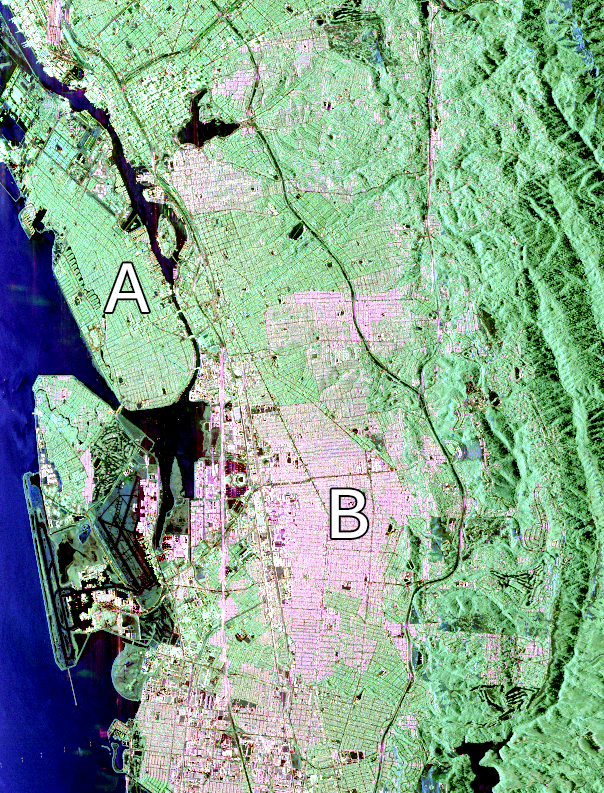
\includegraphics[width = 0.6\columnwidth]{Figures/Trento/ExampleOrientation}
%	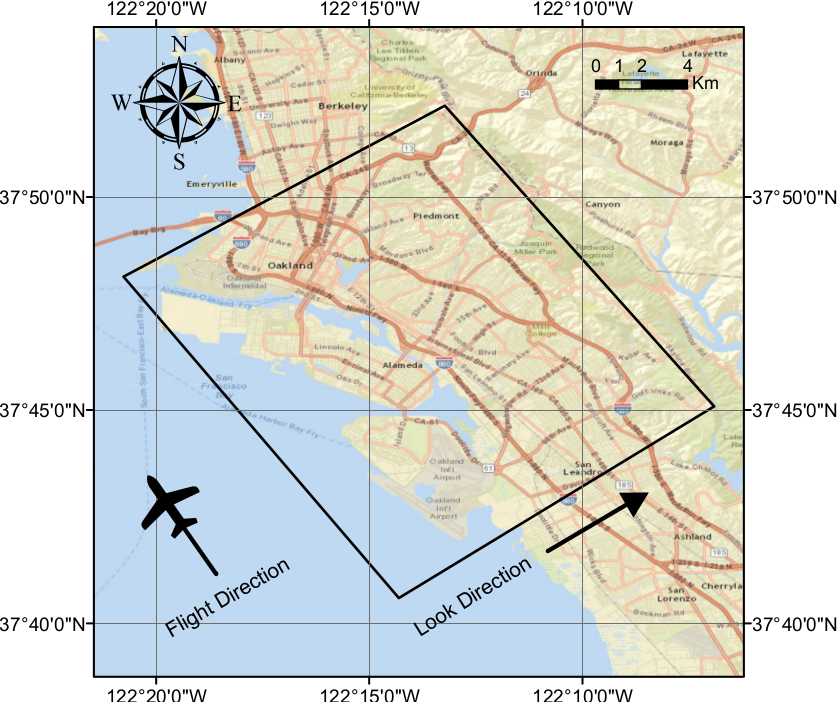
\includegraphics[width = 0.80\columnwidth]{Figures/Map} \quad
	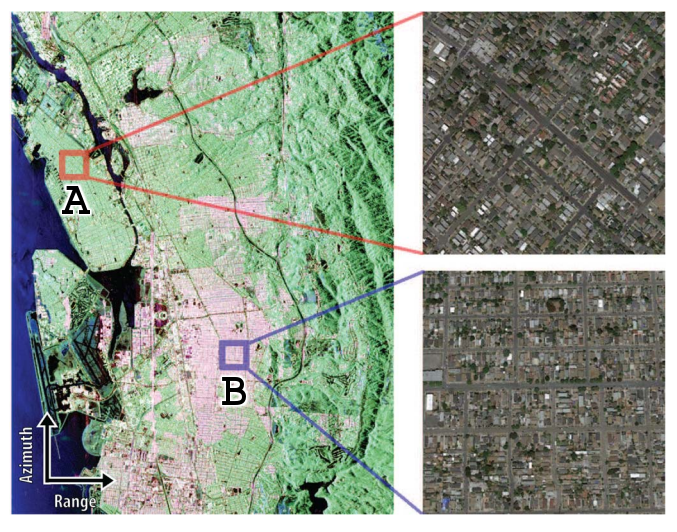
\includegraphics[width = 0.75\columnwidth]{Figures/Trento/UrbanProblem2}
	\caption[PolSAR orientation problem]{Pauli composite generated from UAVSAR polarimetric data-take acquired over Oakland, CA is show along with optical data from Google Earth. Area $A$ is oriented with the radar line of sight while area $B$ is not.}
	\label{fig:orientationExample}
\end{figure}


%DL algorithms
\begin{figure*}[tp]
\centering
		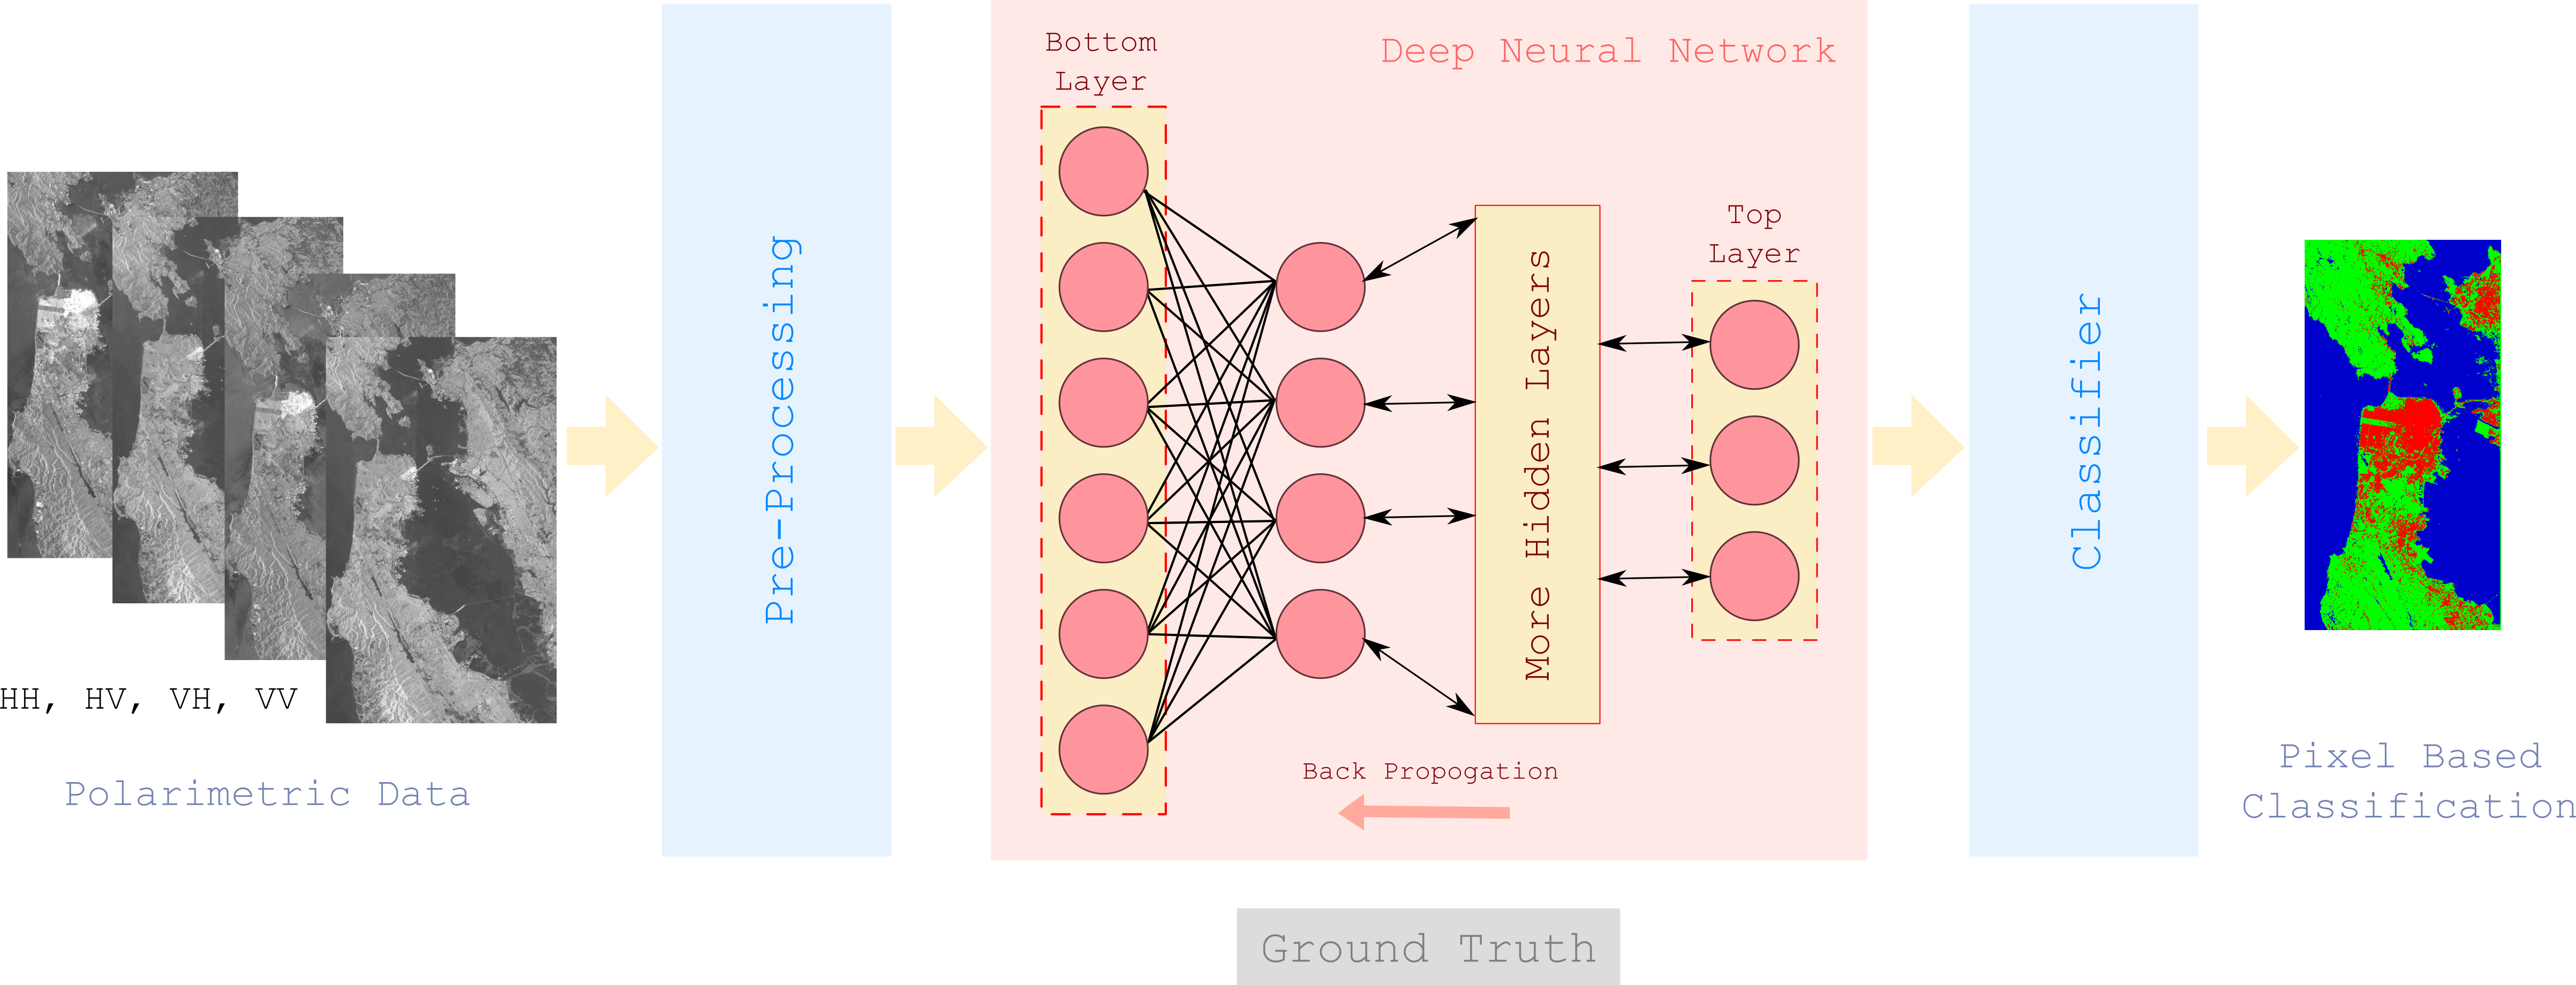
\includegraphics[width=0.85\columnwidth]{Figures/Trento/OverallDL}
		\caption{Framework for pixel classification of PolSAR images using a deep learning architecture.}
		\label{fig:GenDL}
\end{figure*}

%% Referenced in Methdology (introduction) to explain
%% the problem of rotation.
%% TO-DO: Add arrows in figure


%% Overall block diagram of the whole methodology
\begin{figure*}[tbp]
	\centering
%	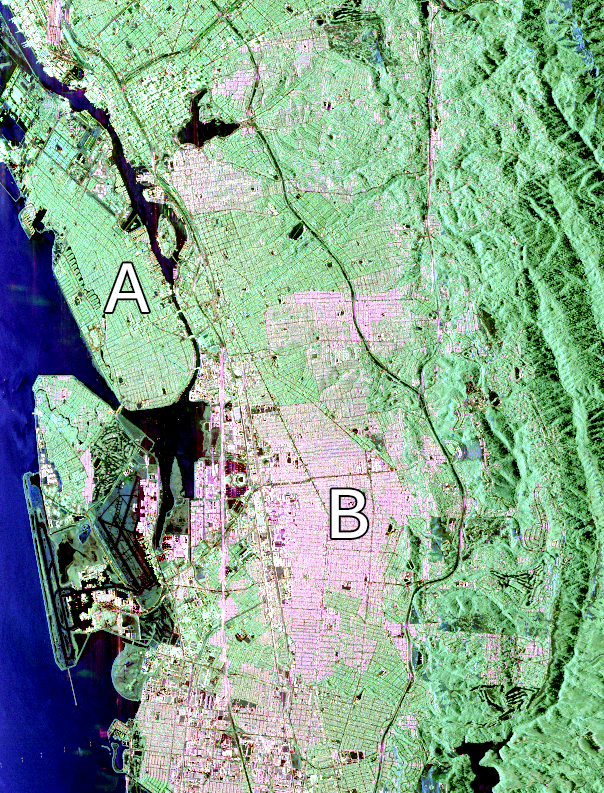
\includegraphics[width = 0.6\columnwidth]{Figures/Trento/ExampleOrientation}
	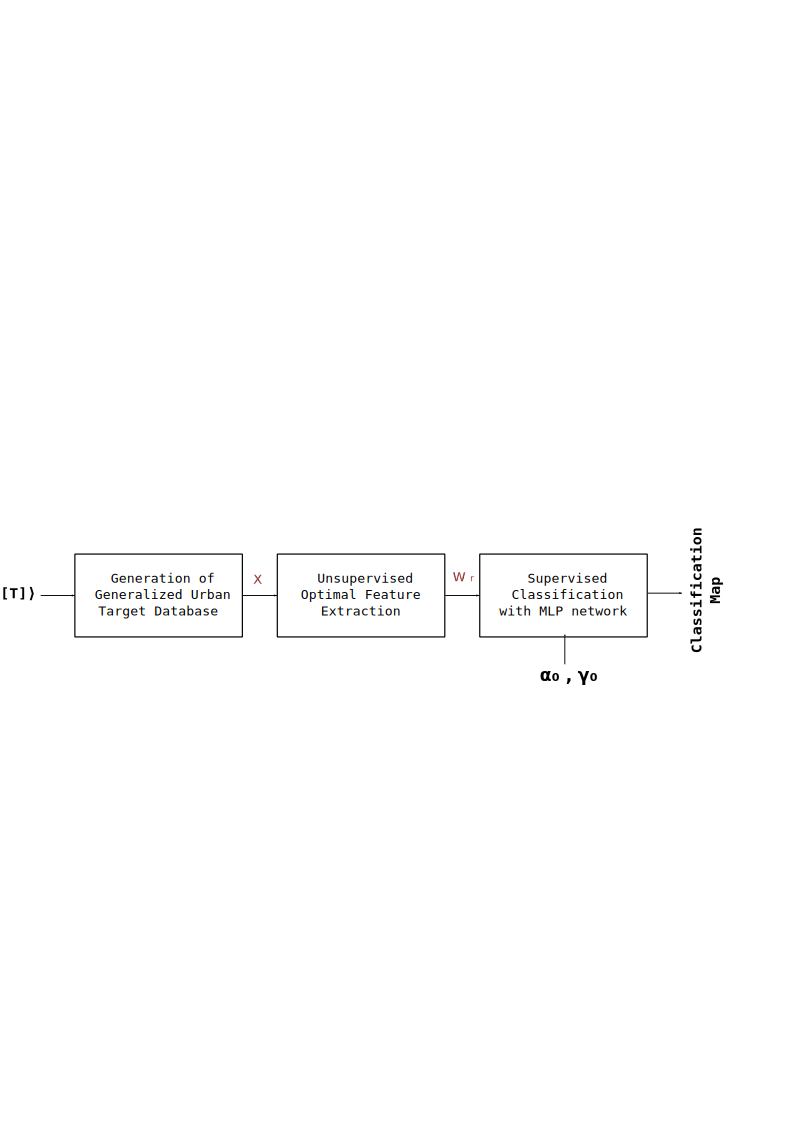
\includegraphics[width = 0.85 \columnwidth]{Figures/Trento/Method0}
	\caption[Overall Methodology]{ Block diagram of the proposed approach.}
	\label{fig:method0}
\end{figure*}

\begin{figure*}[tp]
\centering
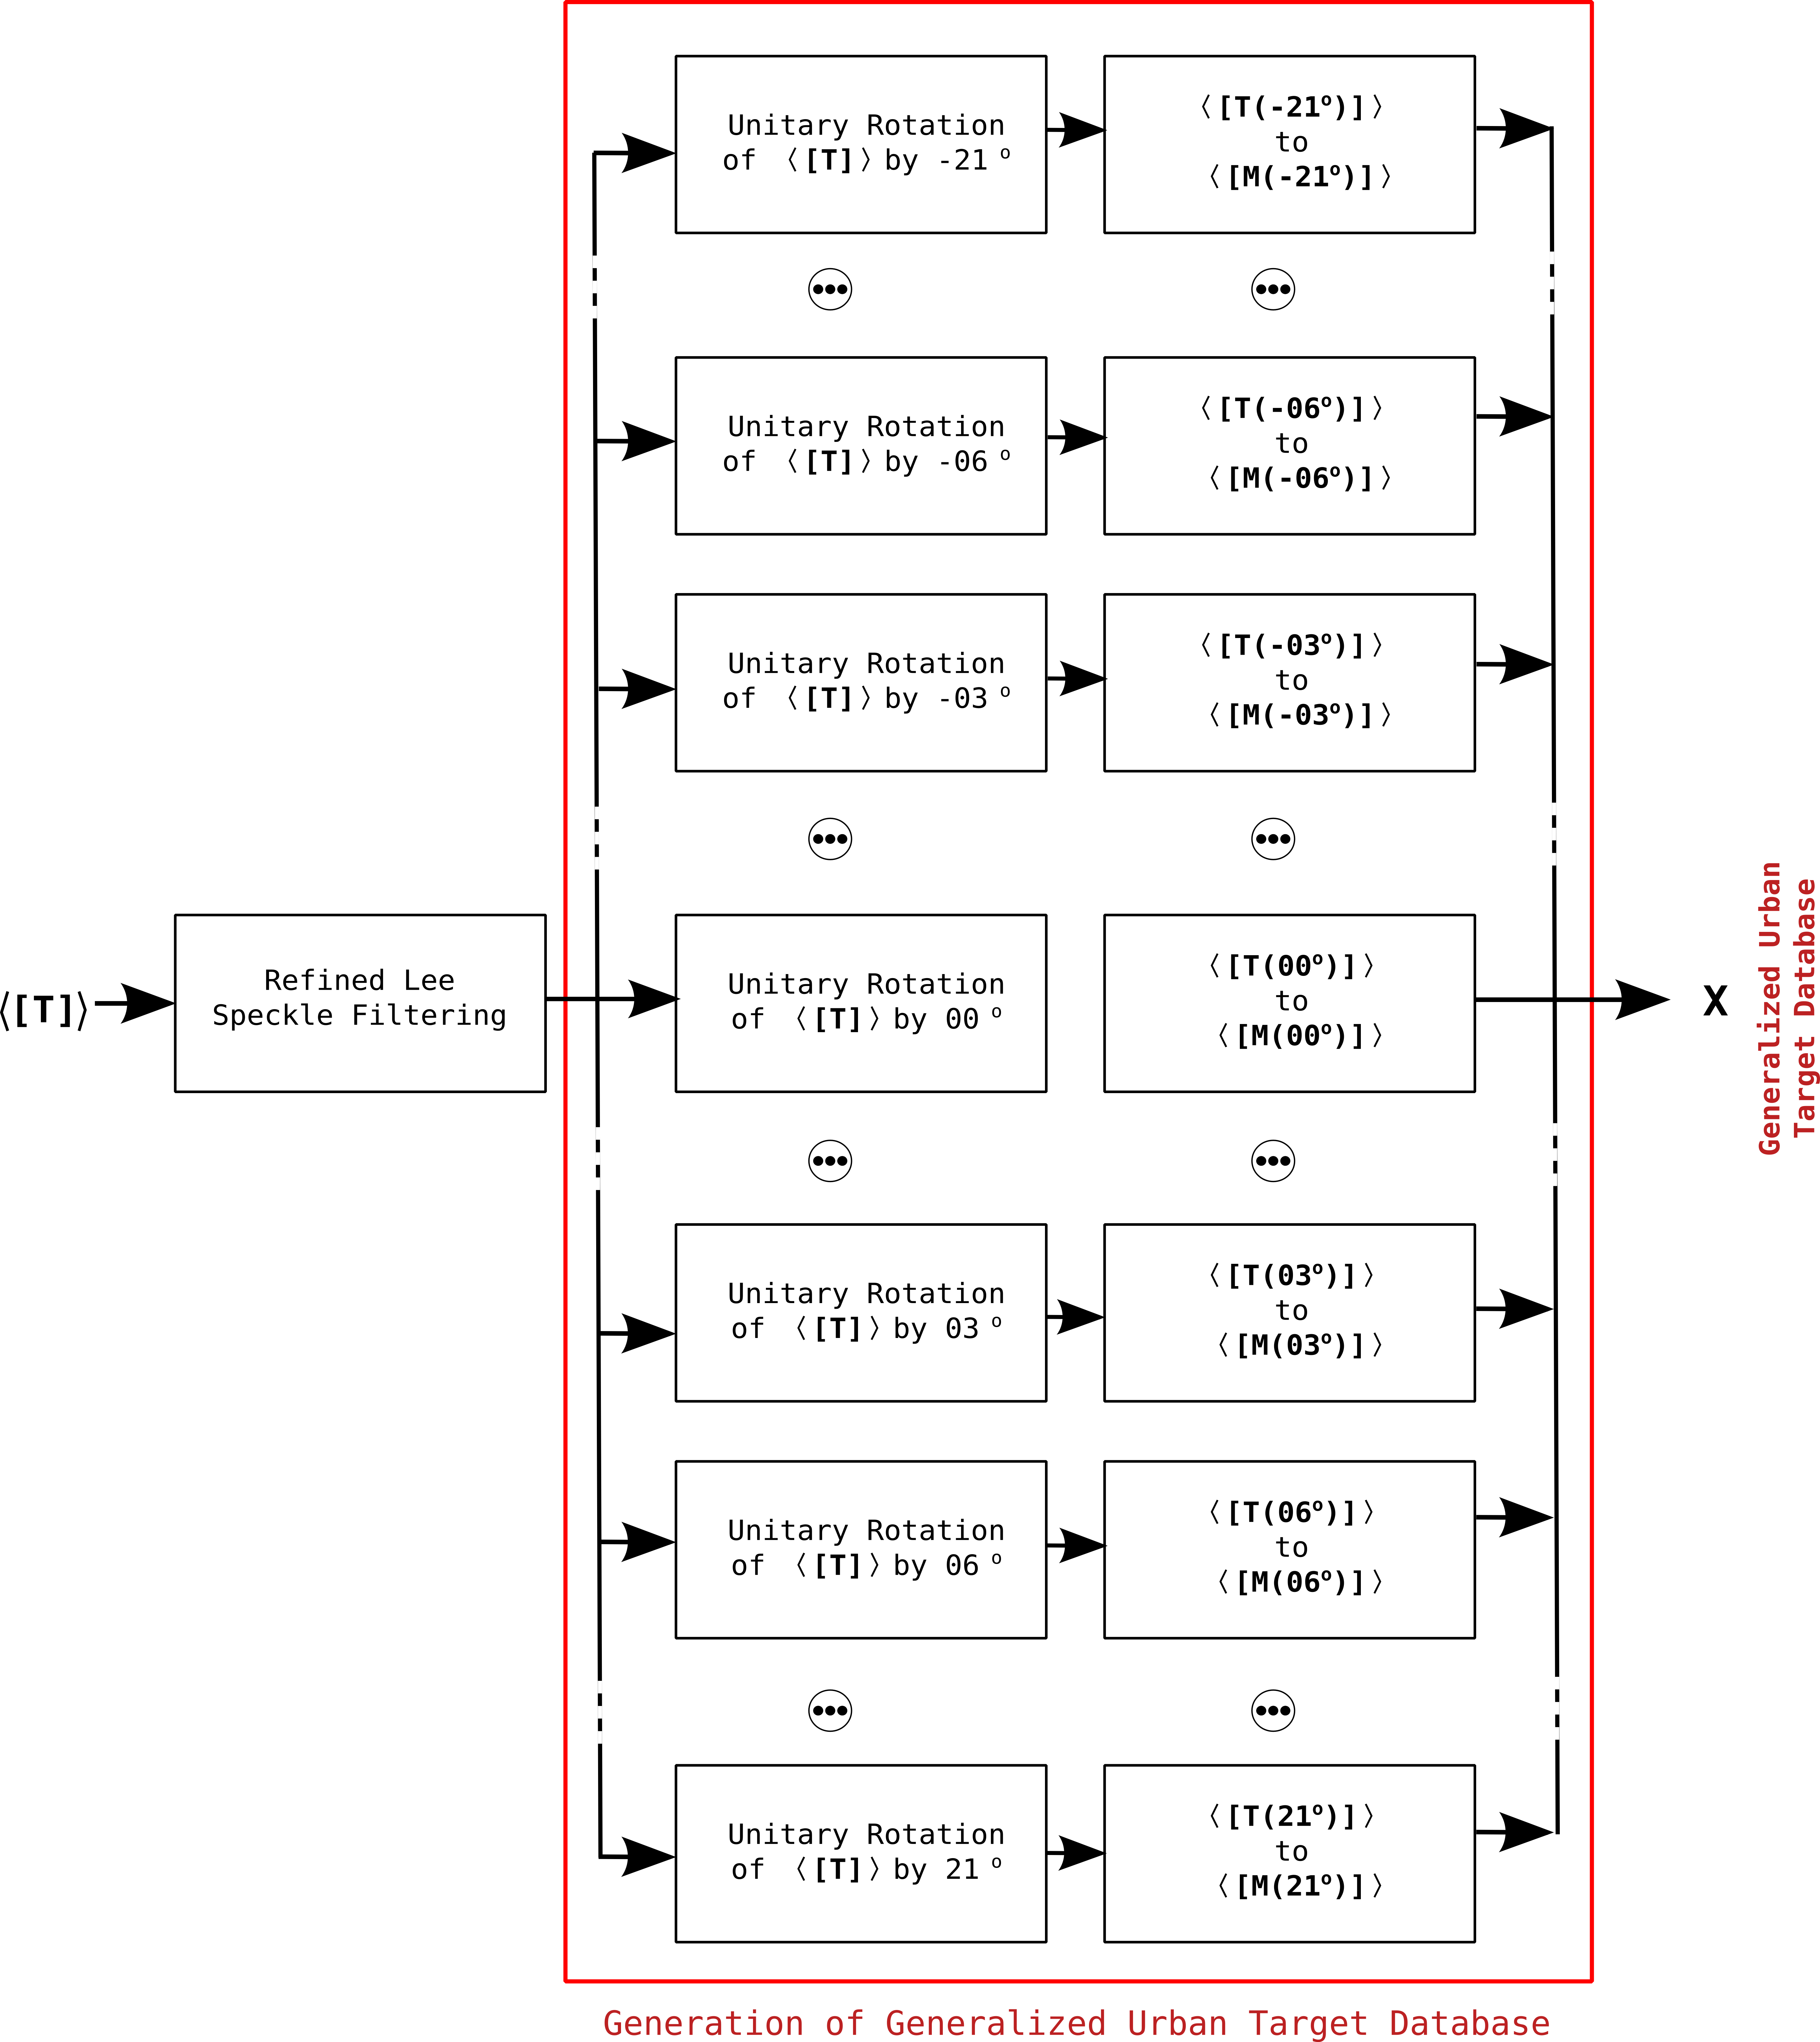
\includegraphics[width = 0.90\columnwidth]{Figures/Trento/Method1}
\caption[PolSAR data preprocessing]{Schematic diagram of the PolSAR data pre-processing and physics based generalized urban target database generation step.}
\label{fig:method1}
\end{figure*}

% % % % % % % % % % % % % % % % % % % % % % % % % %
%             End of Figures                      % 
% % % % % % % % % % % % % % % % % % % % % % % % % %

% % % taking out this header % % % %
%\section{Proposed Classification Approach}


The proposed approach for pixel classification of PolSAR data is shown in Figure~\ref{fig:GenDL}. The polarimetric channels can be considered as low-level input features that describe the geometry and dielectric properties of the target. However, these features are not robust enough to obtain accurate and stable classification performance. A pre-processing step is  applied to transform them  into more robust mid-level features, but this expands the data volume many-fold. A deep learning network is used to extract high-level features which are both efficient and robust with respect to the mid-level ones. In literature both supervised structures such as CNNs~\cite{hu2015deep} and unsupervised structures such as auto-encoders~\cite{chen2014deep}, DBNs~\cite{chen2015spectral} are used to this end. The mid- or low-level features are given as input to the network at the bottom layer and features are extracted from either the top or intermediate layers.  The  features are then classified using a suitable supervised classifier. In general, there are two kinds of classifiers. Hard classifiers such as SVMs which directly produce the classification label as output at every pixel, and soft classifiers such as logistic regression that can fine-tune the whole pre-trained network and predict the class labels as a probability.
The proposed method aims at classifying PolSAR images to identify urban areas and separate them from their surrounding land-cover classes, forest, bare-soil and water bodies. Segmented urban area maps can subsequently be used to characterize urban density, land-area usage, urban sprawl, and land cover change in temporal data amongst other applications. 

The difficulty in the classification of urban areas from PolSAR data arises because of the complex scattering of the polarized radar pulse from urban structures~\cite{kimura2008radar}. This is especially pronounced when they are oriented away from the radar line of sight. Range and azimuth slopes can cause the polarization to rotate about the radar line of sight, which causes the erroneous identification of the scattering mechanism. %~\cite{souissi2016analysis}. 
For instance, scattering observed from urban structures oriented away from the radar line of sight exhibit high cross-polarization as shown in Figure~\ref{fig:orientationExample}. This presents a confusion between urban areas and vegetation leading to incorrect classification. To overcome this challenge, a novel synthetic rotation based approach is proposed which simulates other rotated synthetic targets based on those present in the scene. This allows the machine learning algorithm to better generalize, be more robust and successful in discriminating oriented urban areas. 

The classification process consists of three stages as shown in Figure~\ref{fig:method0}. The first stage deals with the pre-processing of the PolSAR data and the generation of a generalized synthetic urban target database by transforming the input data to obtain a more general representation of the target (Section~\ref{sec:stage1}). The second stage is an unsupervised feature learning step, which automatically learns an optimal representation of the generalized database using a stacked auto-encoder network (Section~\ref{sec:stage2}). Finally, the third stage extracts optimal features from the previous stages, along with some statistical parameters and performs a supervised classification by using a multi-layer perceptron (MLP) network (Section~\ref{sec:stage3}). 



% \textcolor{red}{passive voice}we pre-process the PolSAR data. A refined Lee filter is applied for speckle suppression. To overcome the problem of targets oriented with respect to the radar line of sight, we synthetically rotate the input $\bm{T3}$ matrix to obtain a more general representation of the target, and store each of these rotated $\bm{T3}$ matrices. These are then converted to Mueller matrices and used in training the auto-encoder. As shown in subsequent sections, this helps the learning-machine identify urban targets of similar nature, but oriented with different angles, improving the accuracy of the final classification. In the first stage, the PolSAR data is pre-processed and synthetic rotations are applied. This step allows the simulation of targets rotated away from the radar line of sight, based on the targets that are present in the scene, allowing for increased generalization capability of the learning algorithm. The second stage consists of the auto-encoder which automatically learns an optimal feature representation from the input and synthetically generated data. Finally, in the third stage the features extracted from the preceding stage, along with some statistical parameters are classified in a supervised manner using a multi-layer perceptron (MLP) network. 



%----
\begin{figure*}[!htb]
\centering
	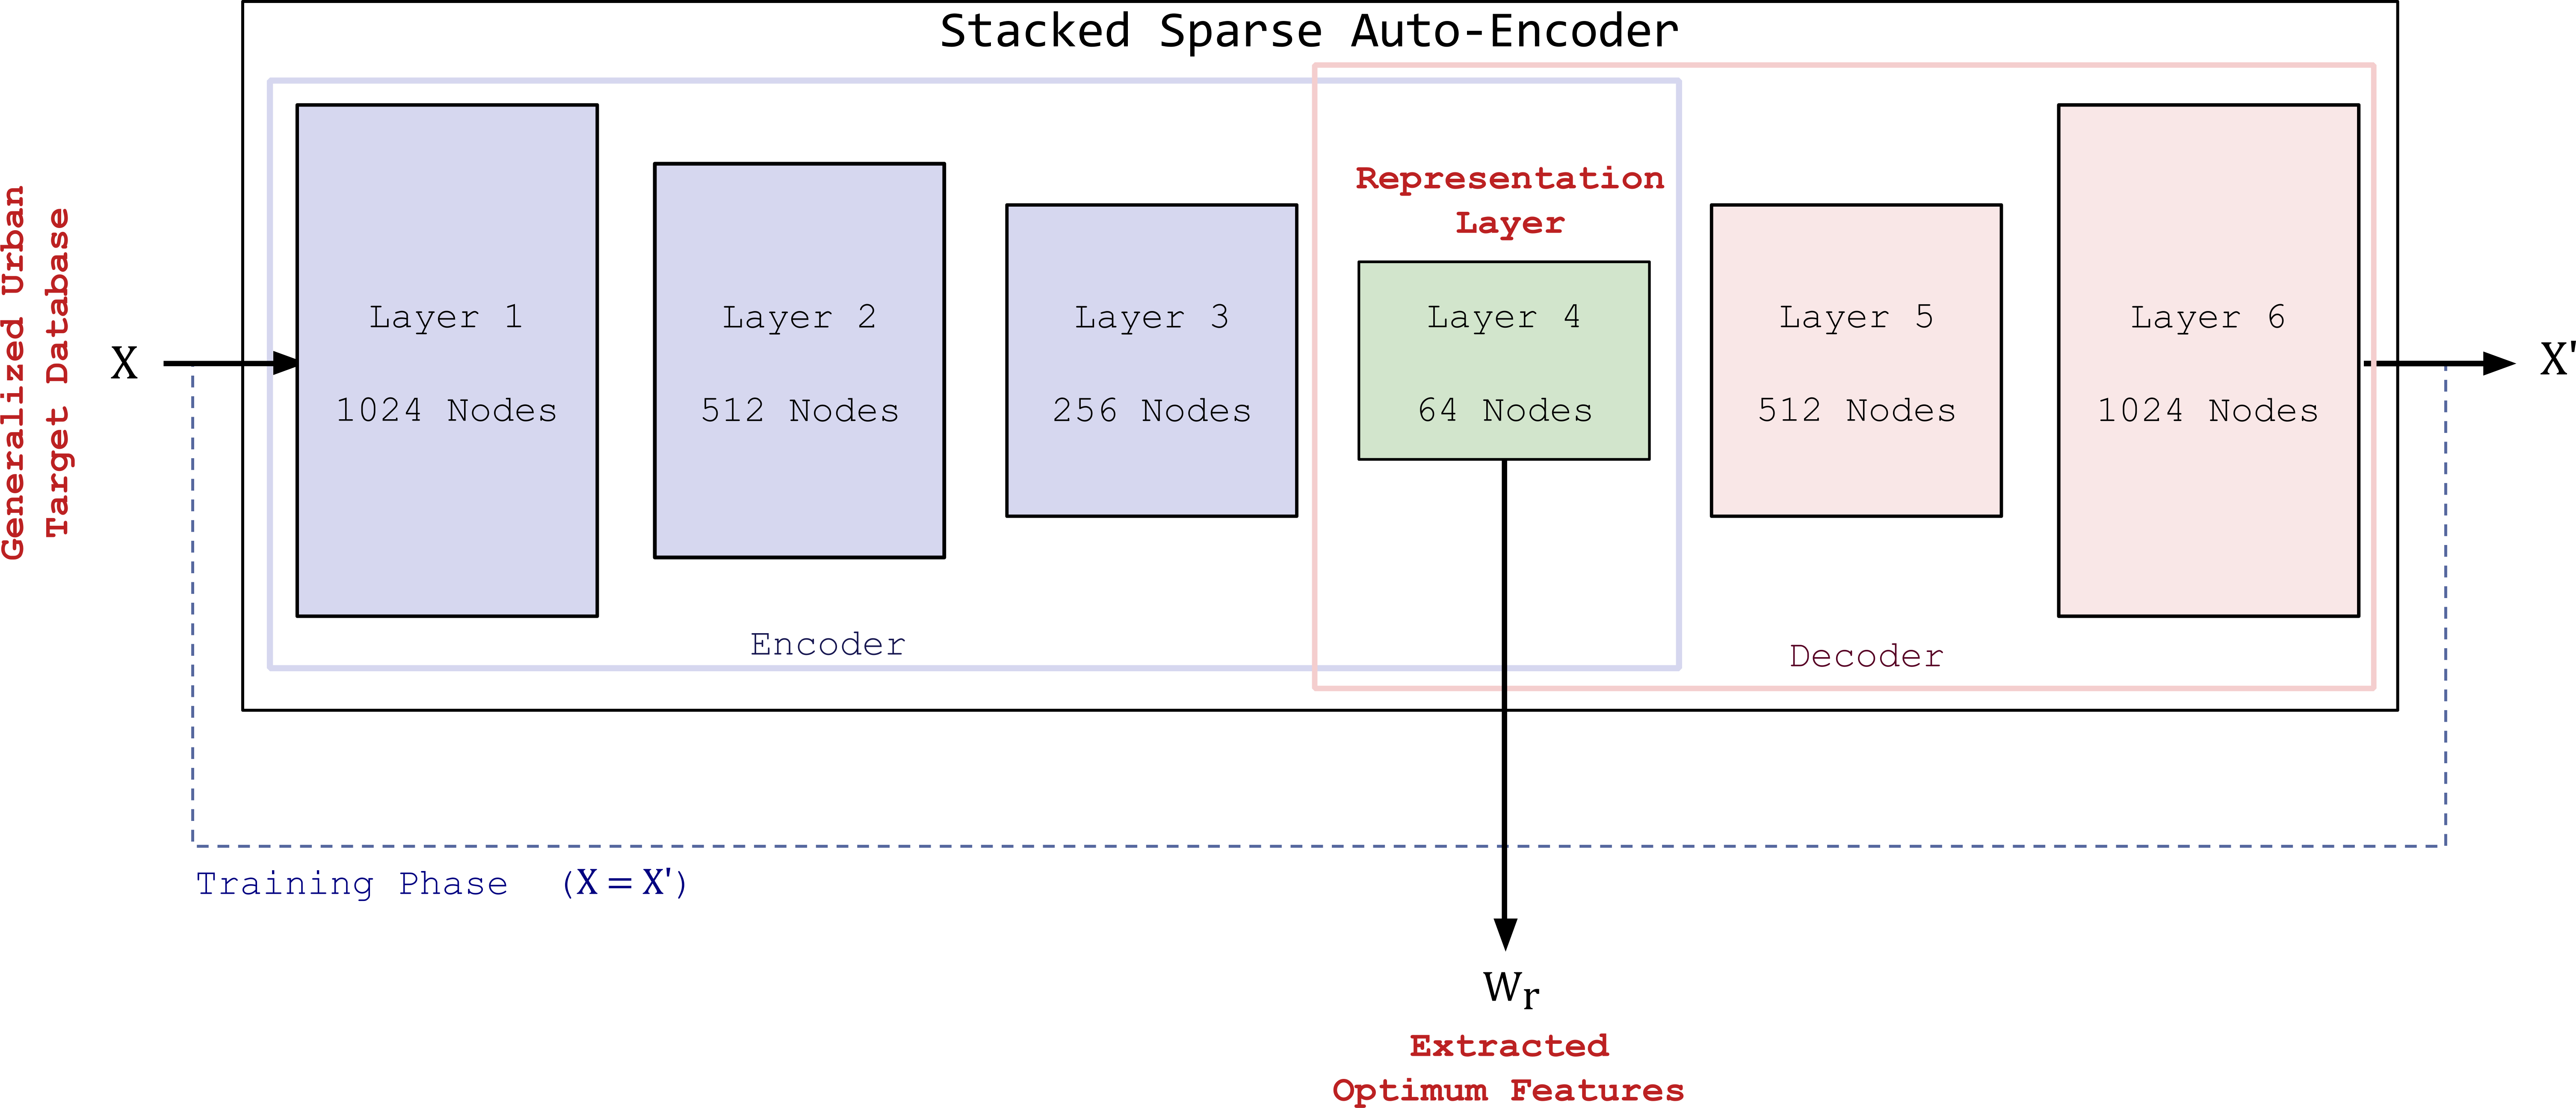
\includegraphics[width = 0.95\columnwidth]{Figures/Trento/Method2}
	\caption[PolSAR data preprocessing Stage 2]{ Auto-Encoder block scheme with Layer 4 extracted as the output feature-set. }
	\label{fig:method2}
\end{figure*}



	
%\subsection{Generation of Generalized Synthetic Urban Target Database}
\subsection{Data Preprocessing}
\label{sec:stage1}



%The first stage of the classifier is represented in Figure~\ref{fig:method1}. PolSAR data is made available from the sensor as a calibrated scattering matrix as described in Equation~\ref{eqn:scattring}. To utilize polarimetric information, we express the data as a spatially averaged coherency $\langle\bm{T3}\rangle$ matrix. Radar images, as a consequence of their coherent nature, are subject to a speckle pattern~\cite{lee1981speckle}. To suppress this, a Refined Lee speckle filter~\cite{lee1981refined} is applied to the dataset as a pre-processing step. This filter is based on the local statistics of the data, is effective, and has a good edge preservation ability allowing the retention of details~\cite{lee1994speckle}. The filtered $\bm{T3}$ matrix is then rotated by $\theta$ varying from $-22^\circ$ to $22^\circ$. Each rotated $\bm{T3}$ matrix is then converted to it's Mueller representation and the matrices are collated together for input to the next stage of the classifier. In this sub-section we describe the preprocessing applied to the polarimetric data, and the rotation based algorithm which is used to 


Measurement by a fully PolSAR system commonly involves the transmission of horizontally ($h$) and vertically ($v$) polarized radar pulses followed by their coherent reception. The polarization state of an incident electromagnetic wave is altered on scattering from a complex radar target. This alteration is a function of the physical and geometrical properties of the target itself, which in turn can serve to characterize it. This scattering  (or Sinclair) matrix is in the ($h,v$) polarization basis and has the form:


\begin{equation}
\mathbf{S} =
  \begin{bmatrix}
    S_{hh} & S_{hv}  \\
    S_{vh} & S_{vv}
  \end{bmatrix}
 \label{eqn:scattring}
\end{equation}


The full polarimetric scattering matrix is available for each imaged pixel and consists of four independent measurements ($hh$, $hv$, $vh$ and $vv$), with the phase relations between them recorded~\cite{tragl1990polarimetric}. Generally, in polarimetriy it is assumed that the targets are reciprocal. In the case of symmetric mono-static scattering, we can thus constrain the scattering matrix to be symmetric, \emph{i.e.} $S_{hv} = S_{vh}$. %The complex Pauli spin matrix basis set ${\{\Psi_P\}}$ can be written as,

%The three unique elements can be used to define a vector of the form: $
%\bm{u} ^\intercal = 
%\begin{bmatrix}
%S_{hh} & \sqrt{2}S_{hv} & S_{vv} \\
%\end{bmatrix}
%$. This vector, $\bm{u}$ has complex number elements. The term $S_{hv}$ is weighed by $\sqrt{2}$ to satisfy the condition that $|\bm{u}|^2$ = span(total power). 

 

%In most radar applications the target is susceptible to some temporal variation. If these variations occur over a time period larger then the illumination time of the radar, the target will appear to be relatively stable. Such targets are said to be deterministic or coherent. The scattering characteristics in this case can uniquely represented by the polarimetric scattering matrix ($\bm{S}$), which completely contains the information about the target at that radar frequency and scattering geometry. 

%However, if the period of the temporal variation is comparable to the observation time of the radar, the target is said to be incoherent or random. This is especially true of natural targets which can be thought of as a volume of a large number of particles moving in a random manner, and are therefore time dependent. Thus when illuminated by a monochromatic radar, the descriptors of the scattered wave, like the amplitudes $a_h(t)$, $a_v(t)$ and phases $\delta_h(t)$, $\delta_v(t)$ are also time dependent. The target thus can be considered to generate a quasi-monochromatic field variations of the scattered waves.  In this case, the target must be characterized by a time average of functions with integration time larger than typical periods of the target's fluctuations~\cite{cox1978ellipsometry}. 

%The Stokes vector representation or the covariance matrix~\cite{cox1978ellipsometry} can be used to describe the statistics of quasi-monochromatic waves. The Stokes formalism can be used to describe the target using the Mueller matrix, which can be related to the covariance matrix by linear transformations~\cite{cloude2009polarisation}.

% %

 
 
%\begin{equation}
%{\Psi_P = \left\{ \sqrt{2}   
% \begin{bmatrix}
%    1 & 0  \\
%    0 & 1
%  \end{bmatrix} 
%  \sqrt{2}   
%  \begin{bmatrix}
%      1 & 0  \\
%      0 & -1
%    \end{bmatrix} 
%    \sqrt{2}   
%    \begin{bmatrix}
%        0 & 1  \\
%        1 & 0
%      \end{bmatrix} 
%  \right\}}
%  \label{eqn:pauli}
%\end{equation}

%The factors $2$, $\sqrt{2}$ or $2\sqrt{2}$ are added in equation~\ref{eqn:pauli} to account for total power invariance with


%\begin{equation}
%Span(S) = |\bm{k}|^2 = |S_{hh}|^2 + 2|S_{hv}|^2 + |S_{vv}|^2
%\end{equation}


The corresponding $\bm{k_p}$-target vector is expressed as,

\begin{equation}
\bm{k_p} = \frac{1}{\sqrt{2}} \begin{bmatrix}  S_{hh}+S_{vv} && S_{hh}-S_{vv} && 2S_{hv} \end{bmatrix} ^T
\end{equation}
where the superscript $T$ denotes transpose. In the mono-static backscattering case, we can construct a $3\times3$ coherency matrix, $\mathbf{T}$, as

\begin{equation}
	\mathbf{T} =  \bm{k} . \bm{k}^{*T} 
\end{equation}


\begin{equation}
\mathbf{T} =  \begin{bmatrix}
t_1 & t_2 & t_3 \\
t_2^* & t_4 & t_5 \\
t_3^* & t_5^* & t_6 \\
\end{bmatrix} 
\end{equation}
where

\begin{align}
\begin{split}
\label{eqn:tmat}
t_1 &=  |k_1|^2   = \frac{1}{2} |S_{hh}+S_{vv}|^2 \\
t_2 &=  k_1k_2^*  = \frac{1}{2} |(S_{hh}+S_{vv})(S_{hh}-S_{vv})^*|^2 \\
t_3 &=  k_1k_3^*  =  (S_{hh}+S_{vv}) S_{hv}^*  \\
%t4 &= \langle k_2k_1^* \rangle = \frac{1}{2} \langle|(S_{hh}-S_{vv})(S_{hh}+S_{vv})^*|^2\rangle \\
t_4 &=  |k_2|^2   = \frac{1}{2} |S_{hh}-S_{vv}|^2 \\
t_5 &=  k_2k_3^*   =  (S_{hh}-S_{vv}) S_{hv}^*  \\
%t7 &= \langle k_3k_1^*  \rangle = \langle S_{hv}(S_{hh}+S_{vv})^* \rangle\\
%t8 &= \langle k_3k_2^*  \rangle = \langle S_{hv}(S_{hh}-S_{vv})^* \rangle\\
t_6 &=  |k_3|^2   = 2 |S_{hv}|^2  \\
\end{split}
\end{align}



$L$ independent and identically distributed samples are averaged to enhance the signal-to-noise ratio while forming the $3\times3$  $L$-looked $\mathbf{T}$ as,
\begin{equation}
\mathbf{T} =  \langle \mathbf{[T]} \rangle = \frac{1}{L} \sum_{i=1}^{L} \bm{k_{p_i}}.\bm{k_{p_i}}^{*\small T} 
\end{equation}
%The $3\times3$ polarimetric coherency $\mathbf{[T]}$ matrix is a Hermition positive semidefinite matrix. It can the transformed to the $3\times3$ polarietric covarience matrix $\bm{C_3}$ by linear unitary transformations~\cite{lee2009polarimetric}.
where $\langle ... \rangle$ denotes temporal or spatial ensemble averaging, under the assumption that the signal is ergodic. 
%and $N$ is the equivalent number of looks. 
Radar images, as a consequence of their coherent nature, are subject to a speckle pattern. Multilooking allows the exploitation of the second order statistical information while providing preliminary speckle suppression. A refined Lee filter~\cite{lee1994speckle} is applied to the dataset as a pre-processing step to further suppress speckle and improve classification performance. This filter is based on the local statistics of the data and has a good edge preservation ability allowing the retention of details.

%\subsubsection{Rotation of $\bm{T3}$} \label{sec:rotation}


The orientation of the target from the radar line of sight, or the presence of azimuth slopes can induce Polarization Orientation Angle (POA) shifts. These can lead to misinterpretation of the scattering characteristics of the target. This is especially common in urban areas oriented at an angle with respect to the radar line of sight and affects the classification performance. The rotation of the $\mathbf{T}$ can help to optimize and extract more polarimetric information which, in-turn helps to improve the characterization of the target scattering mechanism~\cite{bhattacharya2015adaptive}. 
If we consider a %diffused 
target which is symmetrical about the radar line of sight, the rotation of such a target about the radar line of sight can be represented by the unitary rotation of  $\mathbf{T}$ by a matrix rotation model expressed as
%. This can be expressed by transformation of the general averaged coherency $\mathbf{[T]}$ by a matrix rotation model as given by
%We can represent the effect of target rotation about the line of sight with the 
%Consider now a distributed target which has rotation symmetry around the line-
%of-sight as illustrated in Figure 3.10 [9].
%Consider initially a general form for the averaged coherency T 3 matrix and then
%consider transformation of this matrix to model rotations about the %line-of-sight. We
%then obtain the following expression for the averaged oriented coherency T 3 %(u) matrix:

\begin{equation}
\mathbf{T(\theta)} = \mathbf{R}(\theta) \mathbf{T} \mathbf{R}(\theta)^{-1}
\label{eqn:rotation}
\end{equation}

%\begin{equation}
%\mathbf{\langle[T(\theta)]\rangle} = %\mathbf{R}(\theta)\mathbf{\langle[T]\rangle}\mathbf{R}(\theta)^{-1}
%\label{eqn:rotation}
%\end{equation}
where the special unitary rotation matrix $\mathbf{R}(\theta)$ is given by

\begin{equation}
\mathbf{R}(\theta) = \begin{bmatrix}
1 & 0 & 0 \\
0 & \cos 2\theta & \sin 2\theta \\
0 & -\sin 2\theta & \cos 2\theta
\end{bmatrix}
\label{eqn:rotDeets}
\end{equation}
The orientation angle $\theta$ is estimated either by minimizing the $t_6$ element given in (\ref{eqn:tmat}) ~\cite{981347} or by  maximizing a  stochastic distance measure between the $t_6$ and the $t_4$~\cite{Bhattacharya2015}.  


Conversely, if the $\mathbf{T}$ matrix is rotated using unitary rotation as in~(\ref{eqn:rotation}), it would simulate the effect of physically rotating the target while measuring it with a polarimentric antenna. That is, the result of rotating the target $\mathbf{T}$ by $\mathbf{R}(\theta)$ is the $\mathbf{T}$ matrix that would be obtained with target having orientation $\theta$ from the radar line of sight during measurement. Thus, it is expected that by synthetically rotating and storing the rotated $\mathbf{T}$, we can generate a database of synthetic targets based on those detected in the scene.  The rotations are done in discrete steps as show in Figure~\ref{fig:method1} before being collated in a database. The granularity of the rotation steps is directly proportional to the size of training dataset and the capacity of generalization. If the rotations are closely spaced, the database will require more memory, but the generalization ability will be enhanced. However beyond a point, the gain in performance is not justifiable by the rise in computational cost. Therefore a step of $3^\circ$ is selected as a trade-off between performance gain and memory requirement, but other choices are possible. When these are used in the training of the learning algorithm, they improve the generalization capability of the network, allowing it to recognize targets with orientation not present in the original training data. Thus, the rotation based synthetic target database creation strategy in conjunction with a deep learning network architecture improves the classification accuracy of urban areas.

%\subsubsection{Mueller Matrix}
The $3\times3$ coherency matrix $\mathbf{T}$, which is hermitian by the nature of its construction, contains complex valued quantities in its off-diagonal elements. In the complex-number space the solution of differentiation is not guaranteed to be analytic. This poses a problem in the back-propagation step while using neural networks. An alternative approach would be to separate the real and imaginary parts of the elements of  $\mathbf{T}$ and use them as input for the network. However, splitting a complex number to process in real-valued neural networks leads to a sub-optimal representation of the domain of the problem~\cite{hirose2006complex}.

To get around it, we convert the complex valued $\mathbf{T}$ matrix to the real valued Mueller representation. 
%This prevents the direct use of back-propagation based machine learning algorithms like neural networks. 
The Mueller matrix $\mathbf{M}$ is a $4\times4$ real matrix, that can be obtained by a linear transformation of the $\mathbf{T}$ matrix as


% % TODO FOOTNOTE SOMEHOW
\begin{equation}
\mathbf{M} = 
\frac{1}{2} 
\begin{bmatrix}
t_1+t_4+t_6 & t_2+t_2^* & t_3+t_3^* & -i(t_5-t_5^*) \\
t_2 + t_2^* & t_1+t_4-t_6 & t_5+t_5^* & -i(t_3-t_3^*) \\
t_3 + t_3^* & t_5+t_5^* & t_1 - t_4 + t_6 & i(t_2 - t_2^*) \\
-i(t_5-t_5^*) & -i(t_3-t_3^*) & i(t_2 - t_2^*) & -t_1 + t_4 + t_6 \\
\end{bmatrix}
\end{equation}

$\mathbf{M}$ is a real valued matrix with $16$ elements, which reduces to $10$ unique real elements assuming reciprocity conditions.  
%The elements of the matrix can be wholly represented by real numbers, 
This property makes the representation suitable for the purpose of feature learning by neural network structures. Additionally the Mueller matrix is also closely related to the physical properties of a target~\cite{barakat1981bilinear}. This makes it a reasonable choice for identifying the scattering mechanism from targets. In this work, each rotated $\mathbf{T}$ matrix is thus converted to its $\mathbf{M}$ representation.  $\mathbf{M}$ matrices are then collated together as a database of synthetically generated generalized urban targets to serve as input to subsequent stages of the learning algorithm.



%Thus in this stage the input $\mathbf{[T_{3}]}$ matrix is synthetically rotated to simulate a variety of targets, then converted to its $\bm{M}$ representation. All generated $\bm{M}$ matrices are collated together to ease the process of input to subsequent stages of the learning algorithm.


%~\cite{SilvaWishart13}

%Jones to S
%Stokes to Jones
%Mueller and stokes

%Advantage of mueller / real numbers
%physical relation - scattering **




%Polarimetric syntheric Aparture Radar data is collected 
%Sar Data
%T3 or C3 matrix
%Rotation of T3 - multiple angles
%What do I mean by rotation

%Conversion to Mueller 
%Muller repn theory

%Training of Auto Encoder
%Network description
%Architecture

% % % % % % % % % % % % % % % % % % % % % % % % % % % % % % % % % % % % % % % % % % % % % % % % % % % % % % % % % % %



%\subsection{Unsupervised Feature Extraction with a Stacked Auto-Encoder Network}
\subsection{Unsupervised Representation Learning using Auto-Encoders} ~\label{sec:stage2}




%\subsection{Autoencoder} 

\begin{figure}[t]
\centering
	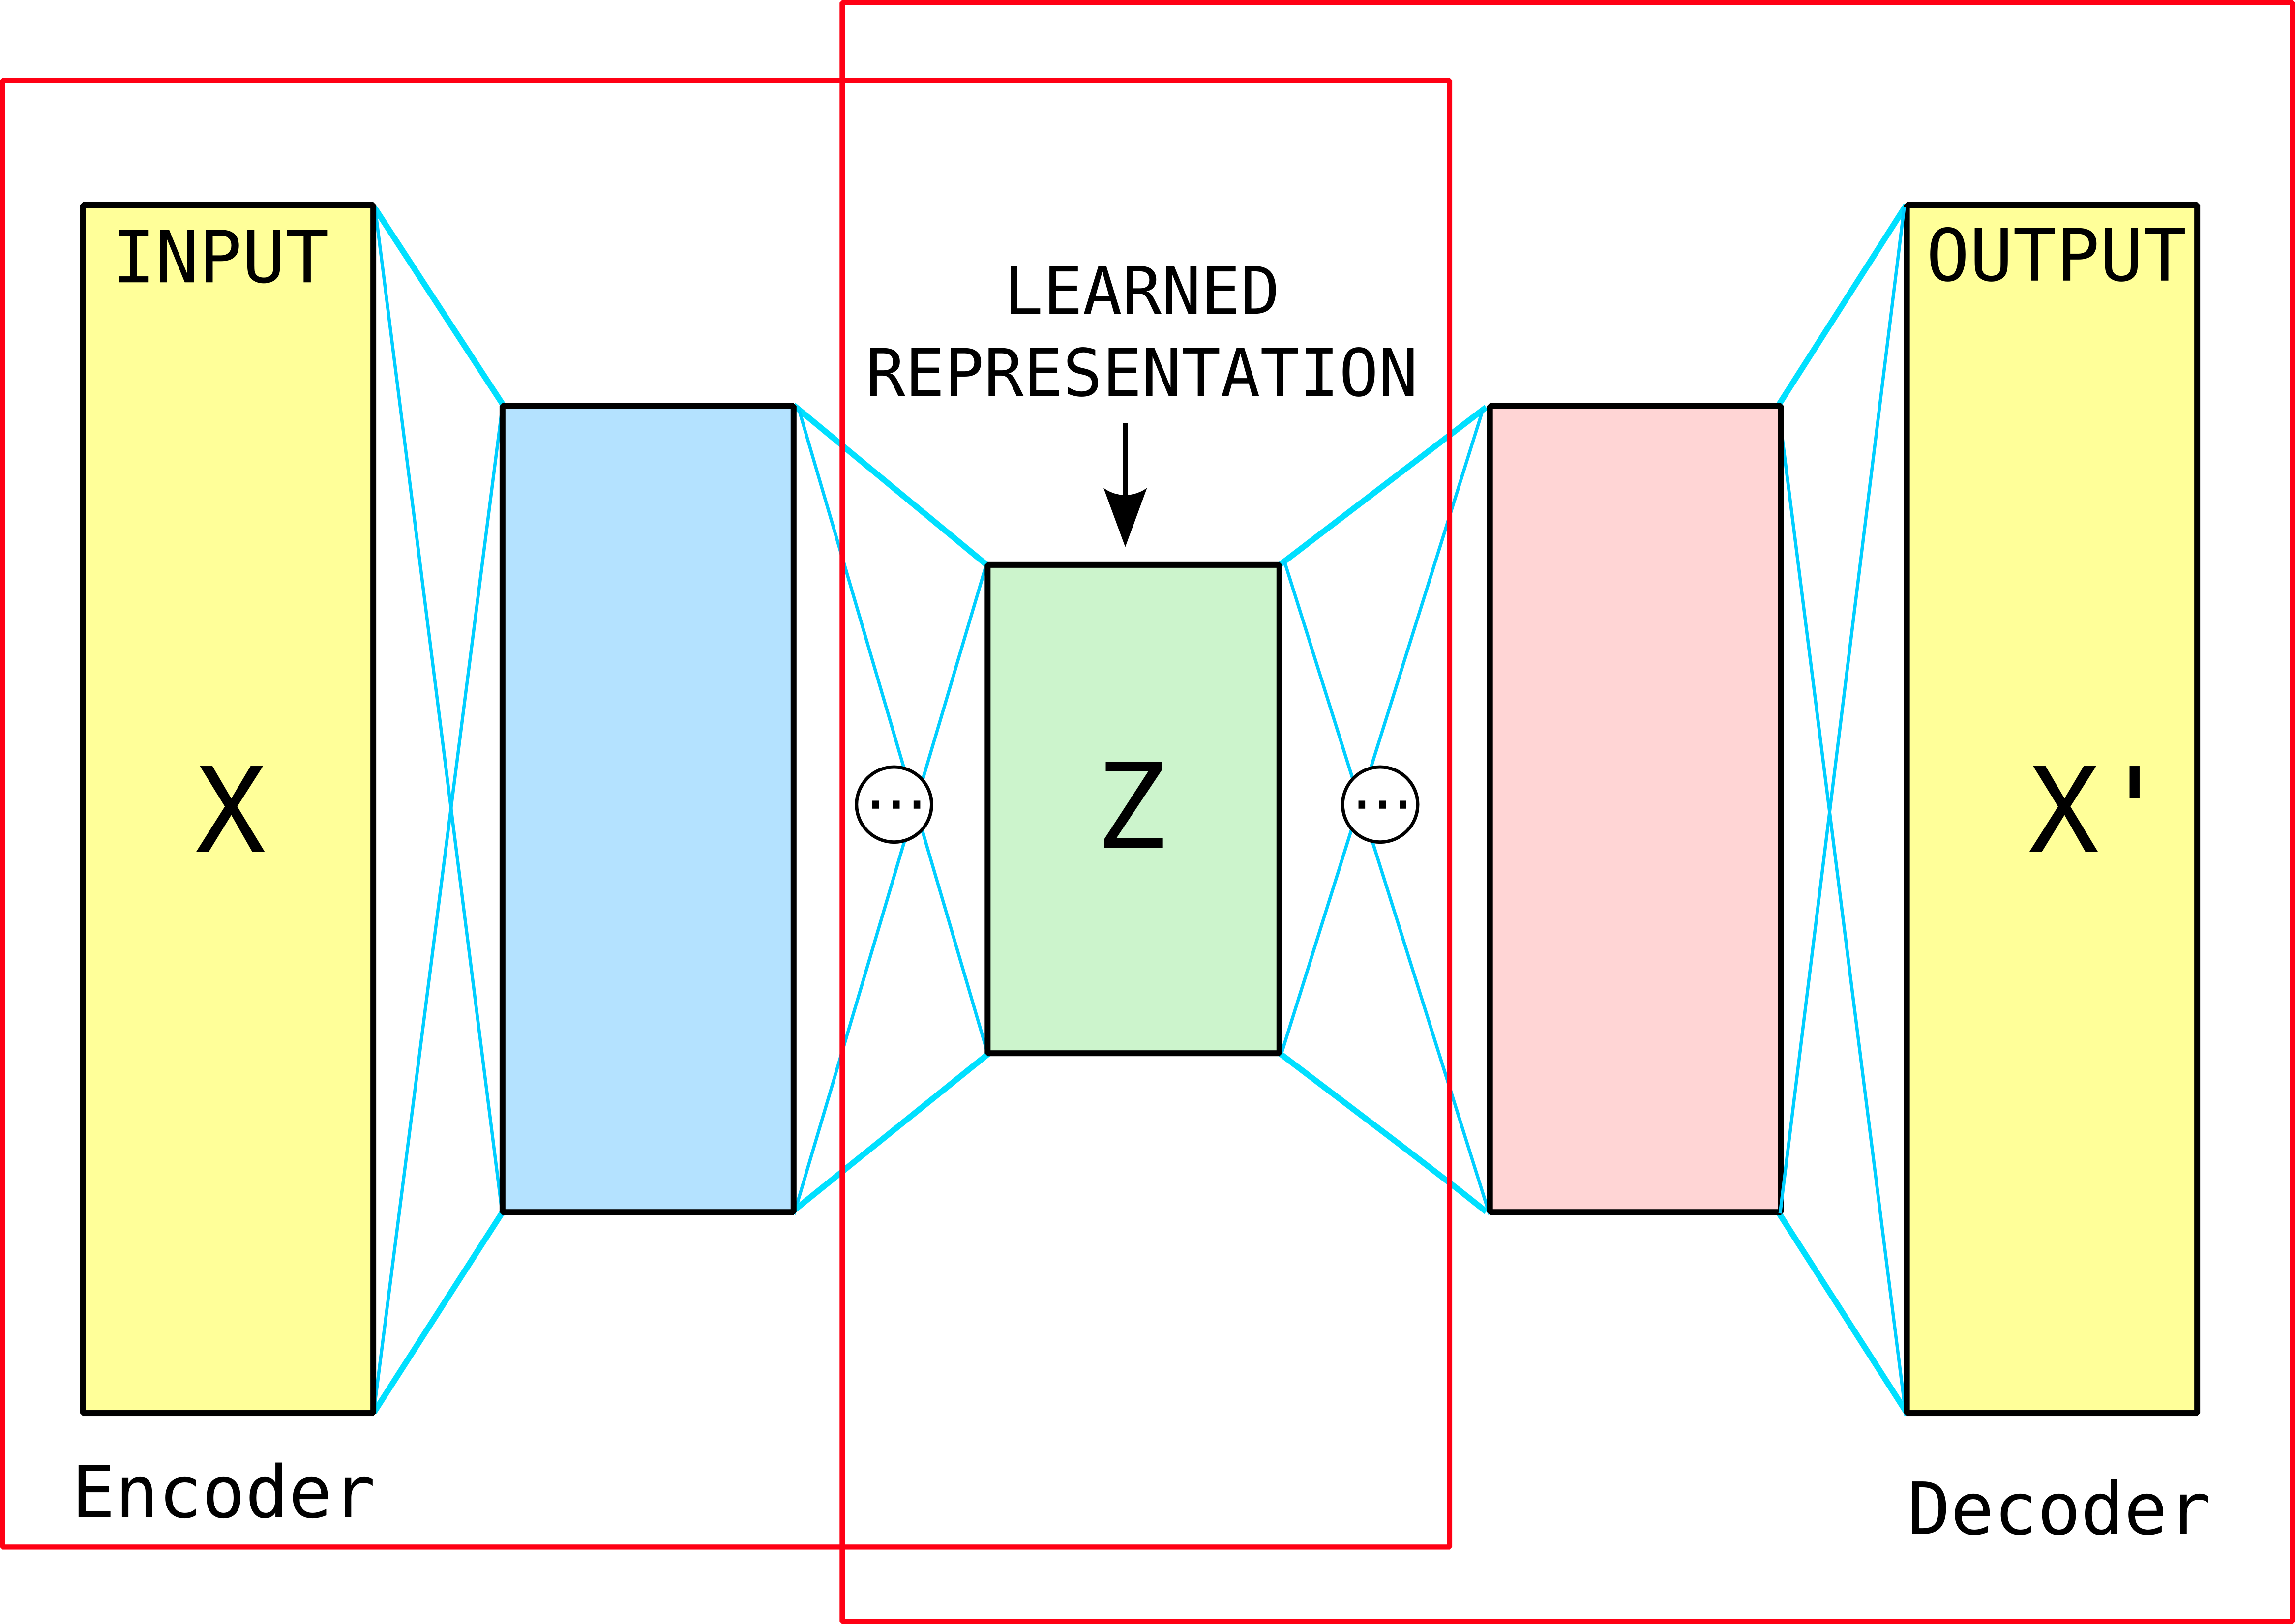
\includegraphics[width = 0.6\columnwidth]{Figures/Trento/AE}
	\caption[Schematic Diagram of an AE]{ Structure of a general auto-encoder with fully connected hidden layers. }
	\label{fig:AE}
\end{figure}

The second stage of the proposed classification method consists of an unsupervised sparse stacked auto-encoder (AE) which is represented in Figure~\ref{fig:method2}. An AE is a feed forward, fully connected, non-recurrent neural network with an input layer, an output layer and one or more hidden layers as shown in Figure~\ref{fig:AE}. 
The output layer has the same number of nodes as the input layer. During the learning phase the AE is trained to reconstruct for each pixel $i$ the input $X_i$ in the output $X'_i$
The error is back-propagated and minimized over multiple iterations. 

The collated synthetic urban target database from the previous stage is made available to the AE as input. The training is carried out  in an unsupervised manner. At the end of the training phase, the weights $W_r$ of the central hidden layer $Z$, are extracted to form an efficient feature representation of the dataset. This stage takes the $n\times10$ dimensional collated target dataset $X$, where $n$ is the number of synthetic rotations, and reduces it to an $m$ dimensional feature set $W_r$, where $m$ is the number of nodes in the representational layer $Z$ and $m < n\times10$. In practice the AE stage integrates information about the rotational response of the target and encodes it into a compact representation. Thus AE acts as an unsupervised feature learning stage and is able to automatically extract an optimized feature set from the input data. This self-learning of the features based on the training data is a hallmark of deep-learning based architectures. This step gives the network  greater generalization ability allowing it to respond to different orientation configurations of the targets. Thus once trained on a target that is  perpendicular to the radar line of sight, it can respond to the same target encountered at an orientation, even if such a configuration was not present in the training samples. %This ability is especially beneficial to classification performance in urban areas because targets, e.g. houses, are very similar in structure but differ in orientation to the radar line of sight. 
%The auto-encoder network used in this study is a 6 layer stacked sparse auto-encoder as shown in Figure~\ref{fig:method2}. The selection of the number of layers were done by training the UAVSAR data-set using the same hyper-parameters and number of nodes though different auto encoder topologies with increasing depth and measuring the lowest cross-entropy error achieved. This is plotted in figure~\ref{fig:layerplot}. We see that a 6-layer auto-encoder was found to be most optimal for this dataset. From input $x$ to output $y$, the network has $1024, 512, 256$ nodes in Layer 1, 2 and 3 respectively forming the encoder, and $128, 512, 1024$ nodes in Layer 4, 5 and 6 respectively forming the decoder. The non-linearity of each encoder is a Rectified Linear Unit (ReLU), allowing the handling of large dynamic range input without saturating.

To understand the action of the AE let us consider a learning problem where a labeled training set $(X_{i},l_{i})$ is available, where $X_i$ represents the input vector and $l_i$ is the corresponding label for the $i^{th}$ pixel. The label is not required for the unsupervised AE stage, but it is necessary for the subsequent classification. The  network consists of  individual neurons that are interconnected such that it is possible to define a complex, non-linear, non-parametric hypothesis $h_{W,b}(x)$.  $W$ is the weight matrix and $b$ is the vector of bias terms for the network. Both these parameters are fitted to the data over the training process. A neuron is a computational unit that takes as input $\bm{X}_i^{n} = X_1,X_2 ... X_n$ and an intercept term $b$, and produces the output, called hypothesis, $h_{W,b}(X) = f(\bm{W^{\intercal}x}) = f(\sum_{i=1}^{n}W_ix_i+b)$, where $f: \Re  \Rightarrow \Re $ is called the activation function or nonlinearity. 

Traditionally the sigmoid $\sigma(x) =  1 / (1+e^{-x})$  has been used as the activation function. It takes a real-valued number $x$ and returns a value within $[0,1]$, according to the magnitude of the input. In practice this has some drawbacks. The output of the sigmoid saturates at either tail of $0$ or $1$ and the gradient at these regions tends to zero, which causes a very small output to be back-propogated. Additionally, if the initial weights are large, the neuron can quickly become saturated during training. The sigmoid function also is not zero centered. During back-propogation if the input data to the neuron is always positive, i.e. $x>0$, then the gradient weights will either become all positive, or all negative. This could introduce undesirable oscillation dynamics in the gradient updates for the weights. To overcome the non-zero centering problem one may use the $\tanh$ activation function, $ f(x) = \tanh(x) = (e^x - e^{-x}) / (e^x + e^{-x})$ which has the limits $[-1,1]$. However this function is subject to saturation when the input has a large dynamic range as it is common in SAR data. 
A non-saturating nonlinearity like the Rectified Linear Unit (ReLU) activation function~\cite{glorot2011deep} can be used to overcome the saturation problem. The ReLU $f(x) = \max(\epsilon,x)$ simply thresholds the data at $\epsilon$, typically $\epsilon=0$. The differentiation of the function is defined as $ \frac{df}{dx} = \{1 : x > \epsilon, 0 : x < \epsilon\}$
%\[
%   \frac{df}{dx} = \left\{
%     \begin{array}{lr}
%       1 & : x > \epsilon\\
%       0 & : x \leq \epsilon
%     \end{array}
%   \right.
%\]  
Another advantage is that the training time for saturating activation functions is larger with the gradient descent algorithm than for its non-saturating counterparts~\cite{krizhevsky2012imagenet}. Since deep learning algorithms use several layers, faster training of ReLU units (as compared to sigmoid or $\tanh$) translates to multi-fold reduction in training times~\cite{nair2010rectified}. Also, the computation of the output of a ReLU is  simple as it does not involve evolution of exponentials like in the sigmoid and $\tanh$, allowing for in-place computation and requiring less computer memory. 
A disadvantage of ReLU units is that, when subjected to large gradients they can update their weights to such a state that they can not be activated by subsequent inputs. The neuron is said to 'die' in the training. To overcome this, the ReLU units can be modified to include a `leakage' term $\epsilon$, $f(x) = 1(x<\epsilon)(\alpha_r x) + 1(x \ge \epsilon)(x)$. This modification causes the units to have a small negative slope, $\alpha_r$ when the input is below the threshold, i.e. $x<\epsilon$. This allows the neuron to recover even if its weight has been updated to a high value by a particular input, over subsequent inputs. The differentiation can be defined as


\begin{displaymath}
   \frac{df}{dx} = \left\{
     \begin{array}{lr}
       1 & : x > \epsilon\\
       \alpha_r & : x \leq \epsilon
     \end{array}
   \right.
\end{displaymath}

The data must be given as input into the AE in random order to prevent it from memorizing the sequence in which the data are presented. The cross-entropy error in each iteration between the output of the AE and the input data is used to monitor the training. A progression towards zero indicates that the network is properly learning, while a stable value indicates that the learning stage is complete. The rate of adaptation of the network is determined by the set learning rate ($\alpha$). $\alpha$ is gradually reduced as the training progress. This is done by multiplying it by a set size multiplier ($\Gamma$). After a given number of iterations $\alpha$ is updated as $\alpha = \alpha \times \Gamma$.  The sparsity of the network is controlled by setting $\rho$, which is the expected activation of a hidden unit averaged across the training samples. As $\rho \rightarrow 0$ the representation becomes increasingly sparse, controlled by the adjustment of $b$. The performance of the stochastic gradient descent algorithm can be improved by introducing of a momentum term ($\mu$). Deep architectures tend to have steep slopes in the objective function near the local optima. This causes the gradient descent to oscillate and leads to a slow convergence. By introducing the $\mu$ term, these oscillations are dampened. 

The AE structure is now a close representation of the input data, and the internal nodes of the AE can be used as features in the classifier. The weights of the representation layer $\bm{W_r}$ of the AE are used as features after completion of the training phase. They are made available as input to the subsequent stage of the method. $\bm{W_r}$ is a sparse representation incorporating possible rotations of the targets present in the scene. This gives it a better generalization ability over the original data-space. A sparse representation also simplifies subsequent classifier design and improves accuracy due to improved inter-class separation~\cite{bengio2009learning}. 

\subsection{Supervised Classification} ~\label{sec:stage3}

\begin{figure}
\centering
	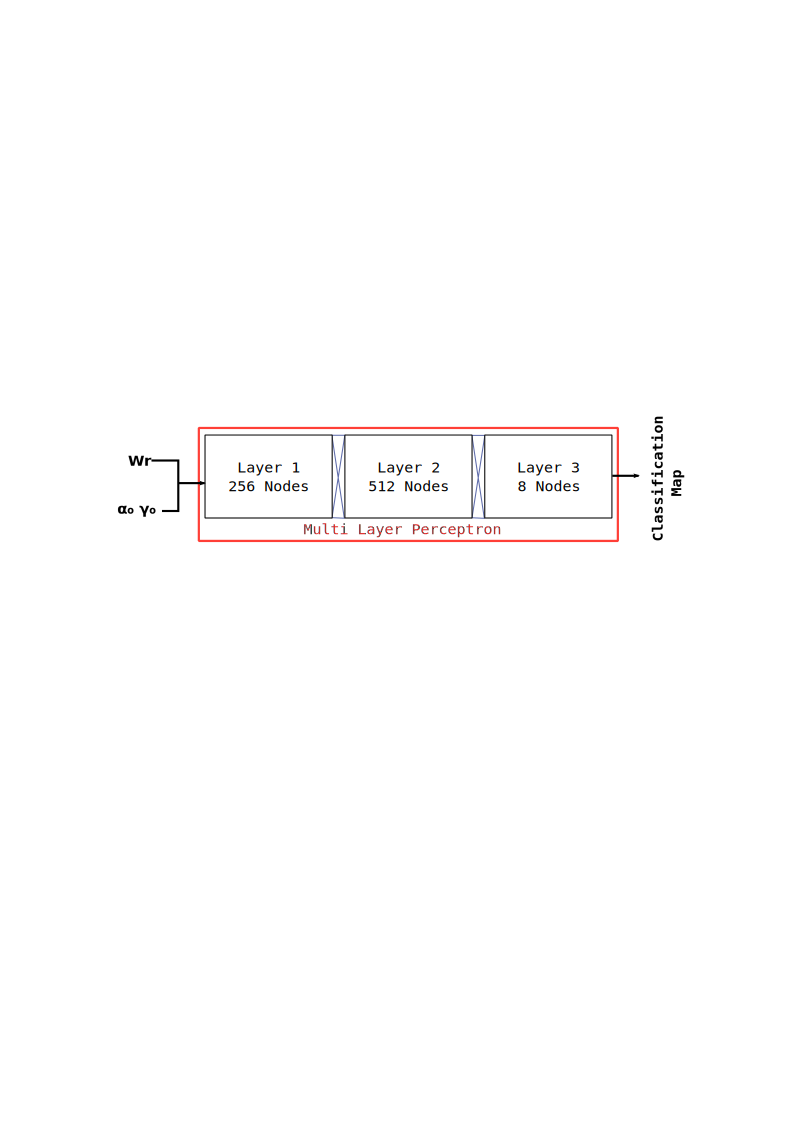
\includegraphics[width =  0.8 \columnwidth]{Figures/Trento/Method3}
	\caption[PolSAR data preprocessing Stage 3]{Stage 3: Final classification is done using a Multi-Layer Perceptron network with parameters extracted from the data.}
	\label{fig:method3}
\end{figure}
	

The third stage of the method consists of a multi-layer percepton (MLP) fully connected feed forward neural network (Figure~\ref{fig:method3}). The network is trained by a supervised learning algorithm that takes training data and labels as input and attempts to classify unlabeled additional unseen data-points. Here, the input to the MLP are the features $\bm{W_r}$ extracted from the previous stage and two statistical parameters $\alpha^0_{ij}$ and $\gamma^0_{ij}$ computed from the data. These parameters are generated by fitting the $\mathcal{G}^0_I$ distribution to the $hh$, $vv$ and $hv$ intensity bands~\cite{Frery97hetroclutter} over a moving window for each pixel ($i,j$) in the image. The three $\alpha^{pq}_{ij}$ and $\gamma^{pq}_{ij}$ parameters are averaged to compute the final values:
\begin{align}
\alpha^0 &= (\alpha^{hh}_{ij} + \alpha^{vv}_{ij} + \alpha^{hv}_{ij} )/3 \\ \label{eqn:stats}
\gamma^0 &= (\gamma^{hh}_{ij} + \gamma^{vv}_{ij} + \gamma^{hv}_{ij} )/3  \notag 
\end{align}
Here $pq$ represents the individual polarization bands ${hh,hv,vv}$ and parameters $\alpha^{pq}_{ij}$ and $\gamma^{pq}_{ij} \in \mathbb{R}$. These statistical parameters add textural context to the classification step improving the accuracy. The $\alpha^0_{ij} < 0$ serves as a measure of the homogeneity (smoothness) of the area while the  $\gamma^0_{ij}$ is the scale parameter of the distribution and thus is related to the brightness of the area~\cite{frery1999models}. For values of $\alpha^0_{ij}$ near zero, the imaged area is very heterogeneous, as in the case of urban areas. The value of $\alpha^0_{ij}$ diminishes to its lowest value for homogeneous areas. The parameter $\gamma^0_{ij}$ can help further discriminate between various type of targets.



The training labels are derived from ground truth information about the area. 
%A small fraction of the total pixels in the scene are used for training to prevent over-training of the neural network. 
%Care is taken to ensure that the training set is representative of the proportions of the land-cover in the scene. 
A three layer network is used to generate the final classification. The network weights and biases are randomly initialized at each iteration using the `Xavier' strategy~\cite{glorot2010understanding}. Since the inputs to this stage have smaller dynamic range, and because the goal is to classify the data into labels, we use sigmoid saturating nonlinearities.   
The network undergoes a training phase using the  labeled samples, extracted features and the statistical parameters. It is iterated to maximize the training accuracy on the test samples. Once the network weights are finalized, the unlabeled pixels in the dataset are classified to generate the  thematic map. 
%In the subsequent section, experimental setup of the methodology, justification for the choice of hyper-parameters and examination of the action of the encoder on the synthetic target database is presented. 
%A three layer network with $256$ hidden nodes in the first layer, $512$ in the second and $8$ in the final layer is used for the final classification. 
 % OK

%% Crop classification methodology


\section{Dataset and Study Area}
\label{sec:stage4}

 Two datasets are primarily used in this study.  A subset (image sub-fragment) of the UAVSAR L-band SAR dataset has been used to study the experiment parameters and actions. The classification is carried out on larger a ALOS-2 L-band SAR image with extensive performance analysis.
 
 
\subsubsection{Dataset Description: UAVSAR L-Band dataset}

The first dataset is a Single Look Complex L-Band UAVSAR dataset acquired over the San Francisco bay area, USA on November 13, 2012, with a resolution of $\SI{0.6}{\m}$ in azimuth and $\SI{1.6}{\m}$ in range. The look angle ranges from $25^\circ$ to $60^\circ$ with a range swath of $\SI{20}{\km}$~\cite{fore2015uavsar}.   This is an air-borne sensor capable of acquiring very high resolution images. The data are multi-looked 3 times in range and 12 times in azimuth to bring them to a resolution of $\SI{7.2}{\m}$ in azimuth and $\SI{5}{\m}$ in range to make them comparable in spatial resolution to the space-borne ALOS-2 dataset. A $1000\times1000$ pixel representative portion is used for these experiments. This data-set is freely available and has similar properties to the space-borne ALOS-2 sensor, so it was used to analyze the action of the network. The subset has a prominent urban area rotated with respect to the radar line of sight, which was used to check the effectiveness of the technique. 

\subsubsection{Dataset Description: ALOS-2 L-Band dataset}
The second dataset is an ALOS-2 image acquired on March 24, 2015 over the city of San Francisco, USA with a resolution of $\SI{3.2}{\m}$ in range and $\SI{2.8}{\m}$ in azimuth. The dataset is multi-looked 3 times in range and 2 times in azimuth to generate an image of resolution $\SI{9.6}{\m}$ in range and $\SI{5.6}{\m}$ in azimuth. The radar operates in L-Band with $\lambda=\SI{24}{\cm}$. The area is heavily urbanized and has high coverage with airborne and space-borne polarimetric radar creating a sizable well documented data-pool that can be exploited for various deep learning techniques. Consequently, this area has been featured in several studies on PolSAR~\cite{lee2004classification, bhattacharya2015adaptive}.

\begin{figure}[htbp]
	\centering
	\begin{subfigure}[t]{0.6\columnwidth}
	\centering
	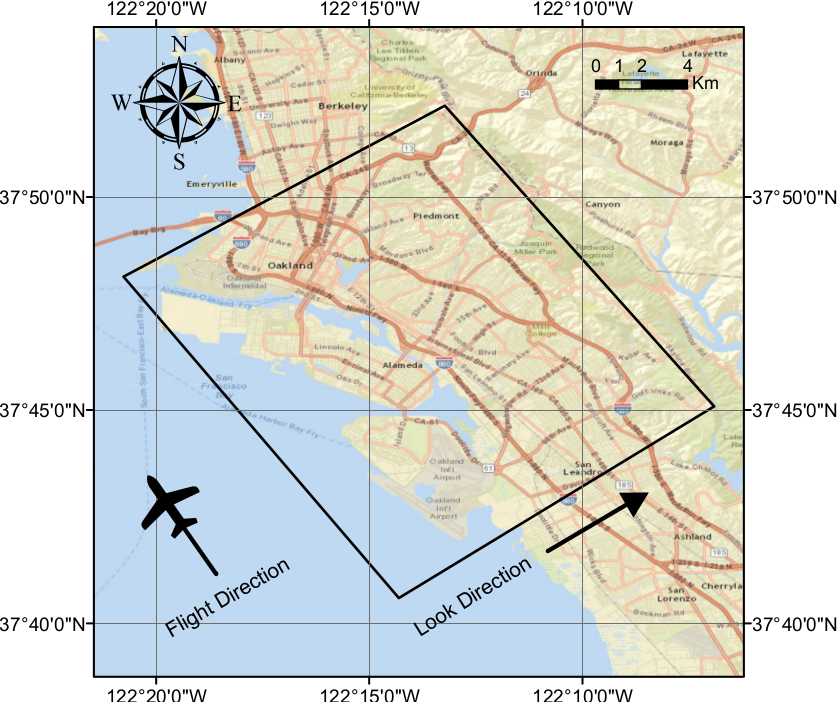
\includegraphics[width =\columnwidth]{Figures/Map} \quad
	%\caption{$\alpha_0$}
	\vspace{-10pt}
	\caption{}
	%\label{fig:alpha}
 	\end{subfigure}%
% 	 ~ 

\vspace{5pt}

	\begin{subfigure}[t]{0.4\columnwidth}
	\centering
	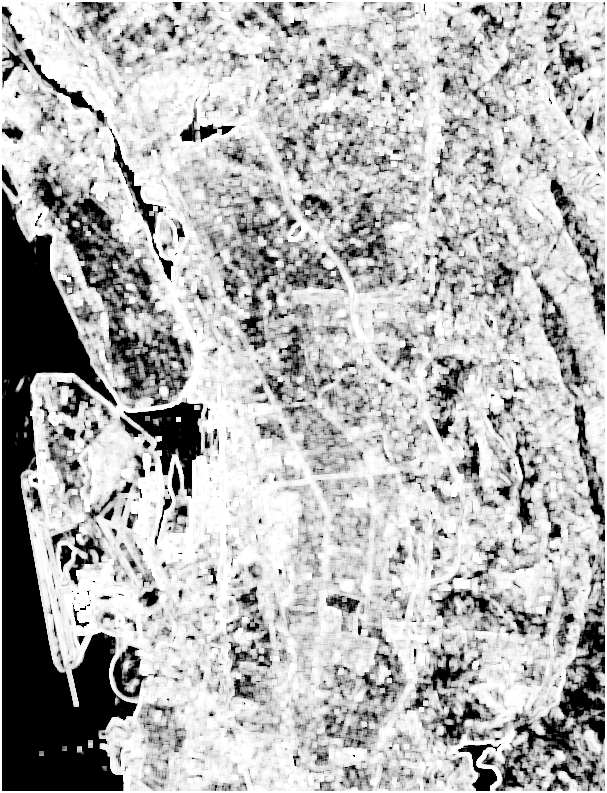
\includegraphics[width = \columnwidth]{Figures/IGRASS15_WORK/alpha_5_5}
	%\caption{$\alpha_0$}
	\caption{}
	%\label{fig:alpha}
	 \end{subfigure}%
	    ~ 
	 \begin{subfigure}[t]{0.4\columnwidth}
	 \centering
	 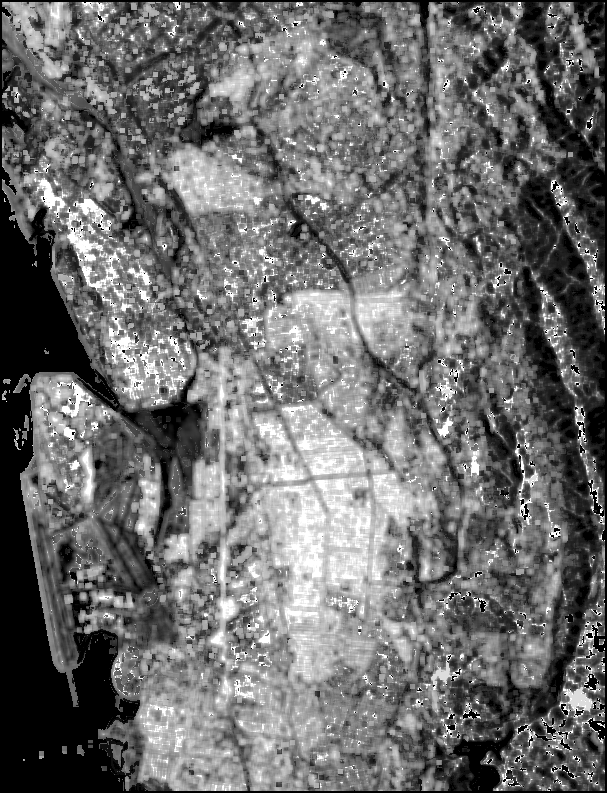
\includegraphics[width = \columnwidth]{Figures/IGRASS15_WORK/gamma_5_5}
	 %\caption{$\gamma_0$}
 	\caption{}
	 %	\caption[PolSAR data preprocessing]{Orientation.}
	 %	\label{fig:gamma}
	 \end{subfigure}   
	 \caption{(a) A map with the dataset footprint shown with the (b) $\alpha^0$ and (c) $\gamma^0$ images extracted from a UAVSAR L-Band dataset collected over Oakland. These serve as textural information to the classifier.}
	 \label{fig:alphagamma}
\end{figure}


By operating in L-Band, ALOS-2 has increased penetration capability and is less susceptible to scattering due to surface roughness. As a result, return from areas of smooth vegetation such as parks and golf courses appear to have undergone specular reflection, and consequently have very low return power levels. The average backscattered power  in these areas for the co-polarized channels, $\sigma^0_{hh} \approx -16\mathrm{dB}$,  and $\sigma^0_{vv} \approx -15\mathrm{dB}$. This is comparable to that of still water, which is about $\sigma^0_{hh} \approx \sigma^0_{vv} \approx -19\mathrm{dB}$ and is much lower than the power returned from forest areas, where $\sigma^0_{hh} \approx 6\mathrm{dB}$ and $\sigma^0_{vv} \approx 7\mathrm{dB}$. Consequently the areas having very low backscatter power tend to be classified as belonging to the water class. This phenomenon is a function of the incidence angle of the sensor and the relative roughness of the surface  with respect to the sensing wavelength. 




\begin{figure}
\centering
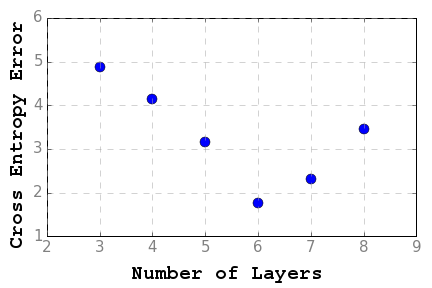
\includegraphics[width=0.6\columnwidth]{Figures/layers}
\caption{Effect of layer depth on training of AE in terms of cross entropy error versus the number of layers.}
\label{fig:layerplot}
\end{figure}




\section{Experimental Set-Up}
\label{sec:expt_cathay312}

`Urban', `Forest/vegetation' and `Water' are the classes chosen in this study. These   classes are usually an important input for various applications related to urban classification. Disaster management studies, urban sprawl estimation, target and infrastructure recognition are examples of applications that benefit from accurate identification of these classes. The urban class comprises of man-made structures which height is equal to or greater than  the sensing wavelength causing the incident EM wave to undergo even number of bounces from the surface surrounding the structure, and  the structure itself before returning back to the sensor. This includes structures like houses, walls, masts etc. These targets are characterized in PolSAR data by a strong double bounce return because of their constituent materials and geometry~\cite{elachi1990radar}.
%In many instances, the challenge in the classification of such a structures is their orientation about the radar line of sight and range or azimuth slopes. In this condition the polarized return, $hh$ and $vv$, is deflected away from the sensor, while a high cross polarized echo is returned. This is generally expected from natural areas such as vegetation causing misclassification.
%The deflection of the polarized return away, and cross polarized echo towards the sensor from urban areas oriented away from the radar line of sight causes it to be confused with natural areas such as vegetation causing misclassification.
In the context of this study, the `Forest / Vegetation' class is used to refer to areas of natural vegetation, open spaces between urban areas with light to almost no vegetation, parks etc. In PolSAR, this class is characterized  by diffused scattering which does not change significantly with rotation about the radar line of sight. The `Water' class is made up of water bodies that are characterized by specular or surface reflection depending on the condition of the surface. At longer wavelengths, some smooth natural areas have a very low return and tends to be misclassified as water. The proportion of such pixels is however under 0.2\% of the total as estimated from the ground truth. 



% SAR preprocessing
As a part of the SAR pre-processing, a refined Lee Filter with a window size of $3\times3$ is applied to the dataset after the application of appropriate multi-looking for the suppression of speckle. The areas under consideration have relatively flat topography, and hence no radiometric terrain correction is applied. Appropriate compensation~\cite{atwood2012improving} may be applied in case of highly undulated areas. 
The synthetic target database is generated by rotating $\mathbf{T}$ with a step size of $3^\circ$ in the range  $-22^\circ$  to $22^\circ$. Considering a finer sampling of $1^\circ$ increases the data volume many-fold without a corresponding appreciable increase in classification accuracy.

The network used in stage 2 of the proposed method is a six layer stacked sparse auto-encoder. To determine the optimal number of layers the dataset was trained on different AE topologies of increasing depth, but with the same hyper-parameters ($\alpha=0.01,\Gamma=0.1,\mu=0.95$). The cross-entropy error at the end of training was analyzed to compare the architectures. From the plot in Figure~\ref{fig:layerplot} it is seen that a 6-layer auto-encoder is the most suitable for this dataset. From input $X$ to output $X'$, the network has $1024,\ 512,\ 256$ nodes in layers 1, 2 and 3, respectively, forming the encoder, and $512,\ 1024$ nodes in layer 5 and 6 forming the decoder. The central $64$ node layer 4 contains the learned representation. The non-linearity of each encoder is a ReLU with a leakage parameter $\alpha_r = 0.01$ allowing the handling of large dynamic range input without saturating or becoming non-responsive over many iterations. The sparsity hyper-parameter of the network is set to $\rho = 0.15$ which ensures that the average activation of each hidden neuron  is approximately near 0. %This is achieved with the addition of a penalty term to the objective function. 
The network weights and biases are randomly initialized at the beginning of each iteration using the `Xavier' strategy~\cite{glorot2010understanding}.
The network is iterated $200,000$ times with a batch size of $1000$. This ensures that the complete data set is passed multiple times though the auto-encoder for better generalization. To ensure that the learning machine is not memorizing the order in which the data are being fed, this order is randomized. The base learning rate is set to $\alpha = 0.001$ and the update step multiplier is set to $\Gamma = 0.1$. The step-size is chosen to be $40,000$ to allow for sufficient number of epochs before the learning rate is updated. The gradient descent momentum is set to $\mu = 0.85$. The value of batch size is adjusted depending on the size of the image. 

In stage 3, a three layer MLP network consisting of  $256$ hidden nodes in the first layer, $512$ in the second layer and $8$ in the last layer is used for the final classification.
When common PolSAR visualization techniques (i.e. Pauli RGB) and decompositions are applied, vegetated and rotated urban areas appear to be visually similar. This makes it more difficult to successfully discriminate and delineate rotated urban areas in a scene as compared to areas that are perpendicular to the radar line of sight.  Hence no training areas are considered from areas which do not show dihedral (red) scattering in the Pauli RGB image. 

The  weights from the representational layer of the previous stage are given as input to the MLP along with and two statistical texture parameters, $\alpha_0$ and $\gamma_0$ (Figure~\ref{fig:alphagamma}).
A window of $9\times9$ has been used for extraction of the parameters. The size of the window is determined by the resolution of the image and dimensions of the targets on the ground. These add more texture information to the classification scheme helping discern urban areas better.  For this network $\alpha=0.01$ (not to be confused with the statistical parameter $\alpha^0_{i,j}$), $\Gamma = 0.1$ and $\mu = 0.95$. About $\sim 5\%$ of the total pixels in the data-set is used for training the MLP. The MLP network is iterated a maximum of 100,000 times.


 



Five experiments are carried out on UAVSAR and ALOS-2 datasets. First, the impact of textural parameters is examined. The AE is trained and the weights of the representational layer are extracted. The MLP classification is performed both with and without the introduction of textural parameters. The difference in classification performance is evaluated in Section \ref{sec:EXPT0}. Second, the impact of the synthetic target generation is studied. The AE is trained on $\mathbf{T}$ as usual. After the completion of training the weight update is stopped and a $\mathbf{T}$ matrix rotated synthetically by $5^\circ$ and $9^\circ$ degrees is given as input. The activation pattern of the neural network in the case of permuted data is compared with the pattern when no rotation is applied (Section \ref{sec:EXPT1}).
Third, classification and performance analysis is conducted on the ALOS-2 dataset (Section \ref{sec:EXPT2}). Accuracy assessment is performed both quantitatively and qualitatively. Fourth, the response of one node of the representational layer is extracted from the AE and plotted to visualize the learned representation  (Section \ref{sec:EXPT3}). Fifth, the results of the proposed method are compared with other classification techniques (Section \ref{sec:EXPT4}).





\section{Results and Discussion}
\label{ref:results1}


The impact of textural parameters and synthetic rotation for target generation on the performance of the network are examined on a subset of the UAVSAR dataset. The analysis of classification performance using the proposed method was conducted on the full ALOS-2 scene along with the analysis of the learned representation. Finally, the performance of the proposed technique was compared with state of the art classifiers for PolSAR data. 


%The proposed technique is evaluated on a full ALOS-2 scene and compared to other polarimetric SAR classification techniques. 




\begin{figure}[tbp]
	\centering
	%	\begin{subfigure}[t]{0.35\columnwidth}
	%	\centering
	%	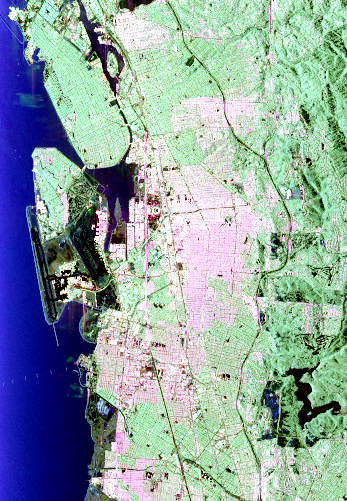
\includegraphics[width = \columnwidth]{Figures/REVIEW/PauliCrop}
	%	\caption{Pauli}
	%\label{fig:alpha}
	%	 \end{subfigure}%
	%	~    
	\begin{subfigure}[t]{0.4\columnwidth}
		\centering
		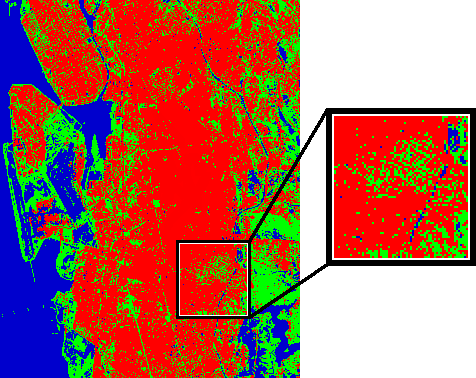
\includegraphics[width = \columnwidth]{Figures/REVIEW/TextureBZ}
		\caption{}
		%\label{fig:alpha}
	\end{subfigure}%
	~ 
	\begin{subfigure}[t]{0.4\columnwidth}
		\centering
		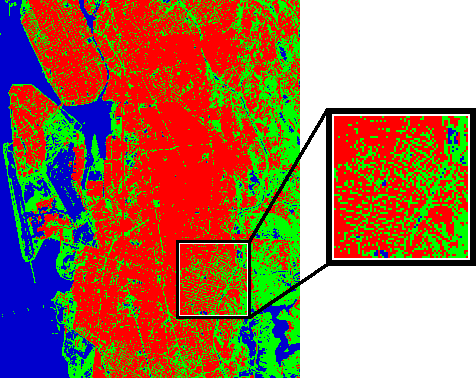
\includegraphics[width = \columnwidth]{Figures/REVIEW/NoTextureBZ}
		\caption{}
		%	\caption[PolSAR data preprocessing]{Orientation.}
		%	\label{fig:gamma}
	\end{subfigure}   
	\caption{Classified map derived from an UAVSAR full polarimetric L-Band dataset (a) with and (b) without the use of $\alpha^0$ and $\gamma^0$ as textural features. }
	\label{fig:texture}
\end{figure}

\subsubsection{Impact of Textural Parameters}
\label{sec:EXPT0}
%%% EDIT THIS
One of the advantages of the deep-learning based approach, is that useful parameters can be included in the later stages of the process. This is in contrast to approaches, where the information must be included at the beginning, causing an increase in dimensionality and classification difficulty, making a feature selection step necessary~\cite{tao2015tensorial,banerjee2014generic}.
Although the inclusion of the textural parameter only slightly improves the overall classification accuracy its inclusion can help discern low-density oriented urban targets. In Figure~\ref{fig:texture} the classification map of the UAVSAR data-set is presented, both with and without the inclusion of the textural parameters $\alpha_0$ and $\gamma_0$ in the MLP stage. The overall improvement in classification accuracy due to the inclusion of textural parameters is small ($\sim 3\%$).  However, for areas of low density sub-urban housing interleaved with vegetation and streets, an improvement is observed (black box in Figure~\ref{fig:texture}) because of benefit from the neighborhood information.  







% % % % % % % % % % % % % % % % % % % % % % 
\begin{figure} [tbp]
	\centering
	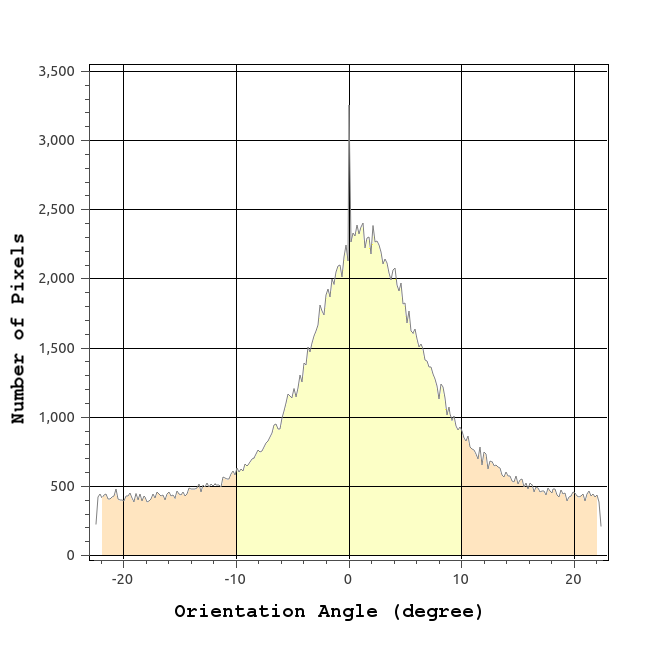
\includegraphics[width = 0.45\columnwidth]{Figures/Trento/orientation_RS2}
	\caption[PolSAR data preprocessing]{Distribution of the estimated Orientation angles of the region imaged in the UAVSAR L-Band dataset acquired over Oakland, USA.}
	\label{fig:orientationHist}
\end{figure} 
%
\begin{figure}[!htb]
	\centering
	\begin{subfigure}[t]{0.31\columnwidth}
		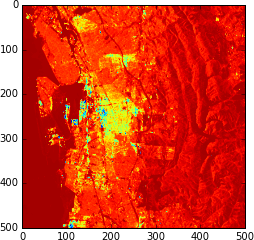
\includegraphics[width = \columnwidth]{Figures/Rotation_FS/0deg_decode3_11}
		\caption{}
		\label{fig:0deg}
	\end{subfigure}%
	~ 
	\begin{subfigure}[t]{0.31\columnwidth}
		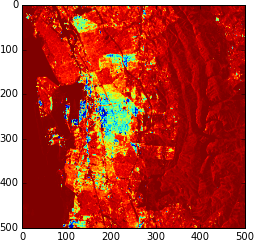
\includegraphics[width = \columnwidth]{Figures/Rotation_FS/5deg_decode3_11}
		\caption{}
		\label{fig:5deg}
	\end{subfigure}   
	~ 
	\begin{subfigure}[t]{0.31\columnwidth}
		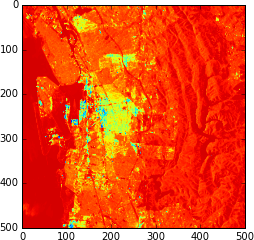
\includegraphics[width = \columnwidth]{Figures/Rotation_FS/9deg_decode3_11}
		\caption{}
		\label{fig:9deg}
	\end{subfigure}  
	
	
	%\centering
	%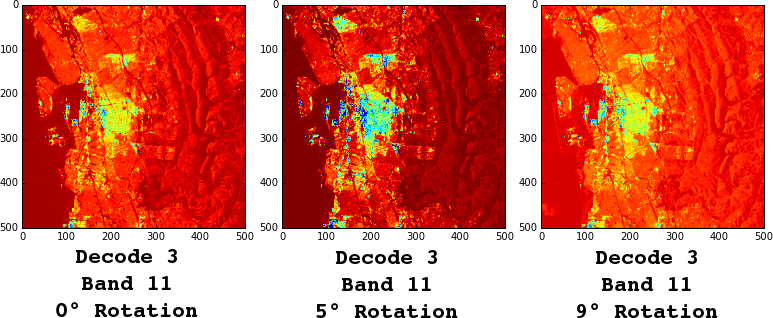
\includegraphics[width = 0.65 \columnwidth]{Figures/Rotation_FS/Rotation} \\
	% The actual value of the output of the ReLU node has been scaled from 0 to 1 for representation as an image.
	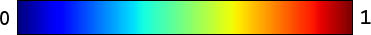
\includegraphics[width = 0.3\columnwidth]{Figures/Rotation_FS/JET}
	\caption[Effect of Rotation]{A section of the UAVSAR image is trained using the auto-encoder network and the extracted features are plotted when input corresponds to a synthetic rotation of (a)  $0^\circ$ (b) $5^\circ$  (c) $9^\circ$ respectively. The actual value of the output of the ReLU node has been scaled from 0 to 1 for representation as an image.  }
	\label{fig:rotCompare}
\end{figure} 

% % % % % % % % % % % % % % % % % % % % % % % % % % % %


\subsubsection{Impact of Synthetic Rotation}
\label{sec:EXPT1}

A histogram of measured orientation angles in the UAVSAR dataset is shown in Figure~\ref{fig:orientationHist}.  It can be seen that most of the targets are oriented between $-10^\circ$  and $10^\circ$. 
%Thus, while generating the synthetic database this range is densely subdivided as compared to the ranges $-10^\circ$  to $-22^\circ$  and $10^\circ$ to $22^\circ$. Between $-10^\circ$  and $10^\circ$ a step size of $3^\circ$ is used, while a step size of $6^\circ$ is used otherwise. 
%Considering a finer and more uniform sampling of $1^\circ$ increases the data volume many-fold without a corresponding appreciable increase in classification accuracy.
The average orientation angle of this subset is approximately $5^\circ $. The orientation angle is computed by the estimation method given in~\cite{981347}. To visualize the action of synthetic rotation, $\mathbf{T}$ is given as input to the trained AE stage after rotation by $0^\circ$, $5^\circ$ and $9^\circ$ degrees separately. As an example, the 11\textsuperscript{th} element of the feature vector is extracted, after completion of the training stage of the AE and is presented in Figure~\ref{fig:rotCompare}. In the case  of the pixels in which the synthetic rotation angle matches the actual target orientation on the ground, the reconstruction error of the AE is lower than the average one over the scene. The areas on the ground that actually correspond to the synthetic rotation ($0^\circ$, $5^\circ$ and $9^\circ$) are closer to zero. The AE was only trained on the input dataset. However it is able to provide an appropriate  response when an unseen and arbitrarily rotated version of the input data is introduced. This implies that the application of synthetic rotation to a target is equivalent to the case when such an oriented target is actually present in the training data. Thus the generalization capability of the AE is improved. 

%the areas of urban structures that were aligned by $5^\circ$ with the radar line of sight have a response closer to zero for the features extracted from the $\mathbf{\langle[T]\rangle}$ matrix which was rotated by $5^\circ$, as compared to the other input cases.   This action allows the AE to respond to a wide range of orientations, even if it is not present in the input data. This effect is exploited in the proposed technique to improve the accuracy of classification.






\begin{figure}[tbp]
\centering
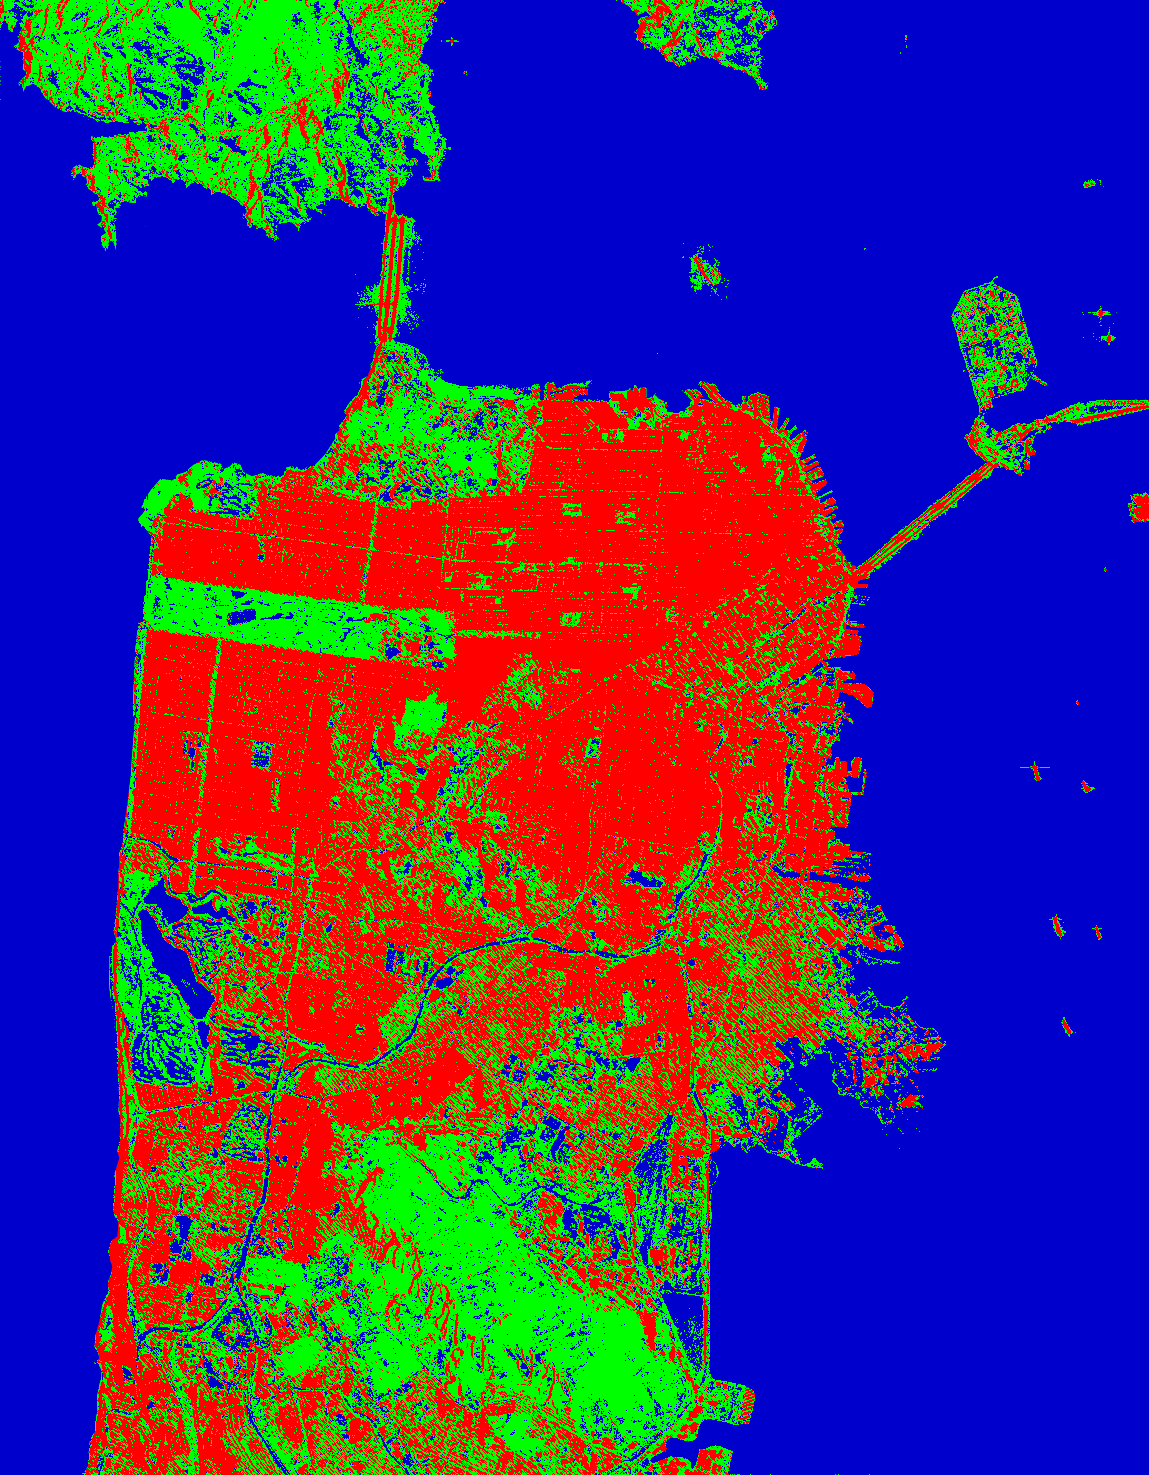
\includegraphics[width=0.5\columnwidth]{Figures/ALOS2_SF_3Class/Output_AL2_500k_alt}



		\begin{tabular}{clclcl}
					
\includegraphics[width=0.03\columnwidth]{Figures/RS2_SF_3Class/Blue.png} & Water &		
\includegraphics[width=0.03\columnwidth]{Figures/RS2_SF_3Class/Green.png} & Forest &  	
\includegraphics[width=0.03\columnwidth]{Figures/RS2_SF_3Class/Red.png} &  Urban 
		\end{tabular}
		
		\caption{Classified map of San Francisco derived from an ALOS-2 full polarimeteric L-Band dataset.}
		
\label{fig:compwal2}
\end{figure}











\begin{figure}[tbp]
\begin{subfigure}[t]{0.19\textwidth}
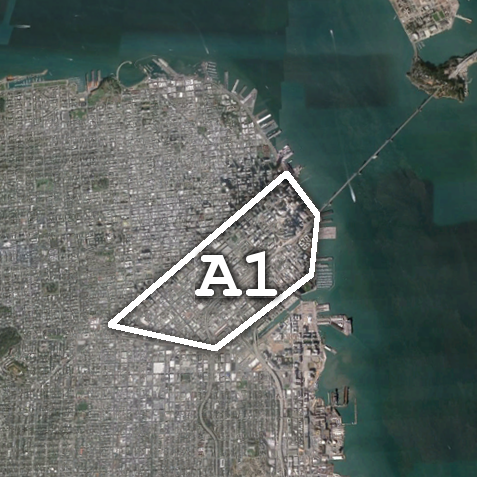
\includegraphics[width=\columnwidth]{Figures/ALOS2_SF_3Class/SouthMarketIm}  
\vspace{0.2cm}
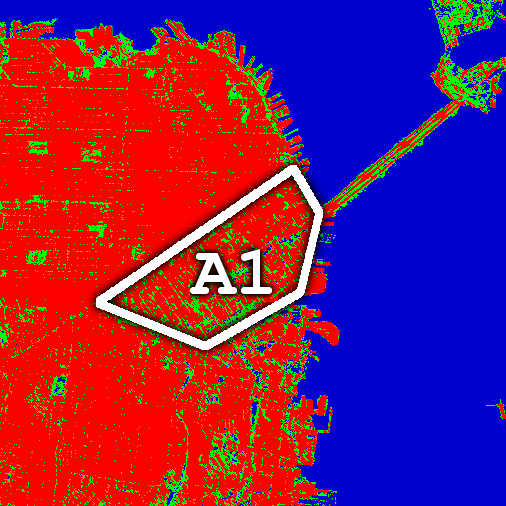
\includegraphics[width=\columnwidth]{Figures/ALOS2_SF_3Class/SouthMarket}
\caption{}
\label{fig:cla2_a}
\end{subfigure}
%\begin{subfigure}[t]{0.31\columnwidth}
%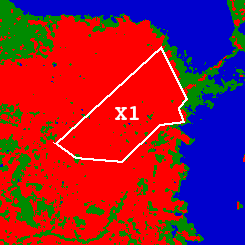
\includegraphics[width=\columnwidth]{Figures/RS2_SF_3Class/SouthOFMarket_Cl}
%\caption{South of Market}
%\end{subfigure}
\begin{subfigure}[t]{0.19\textwidth}
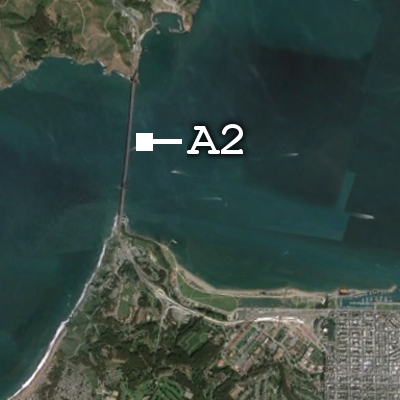
\includegraphics[width=\columnwidth]{Figures/ALOS2_SF_3Class/GoldenGateIm} 
\vspace{0.2cm}
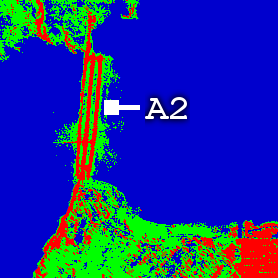
\includegraphics[width=\columnwidth]{Figures/ALOS2_SF_3Class/GoldenGate}
\caption{}
\label{fig:cla2_b}
\end{subfigure}
%\begin{subfigure}[t]{0.31\columnwidth}
%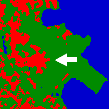
\includegraphics[width=\columnwidth]{Figures/RS2_SF_3Class/sfo_cl}
%\caption{Richmond}
%\end{subfigure}
\begin{subfigure}[t]{0.19\textwidth}
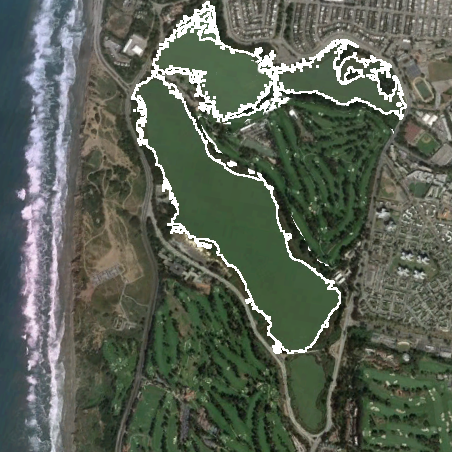
\includegraphics[width=\columnwidth]{Figures/ALOS2_SF_3Class/Lake} 
\vspace{0.2cm}
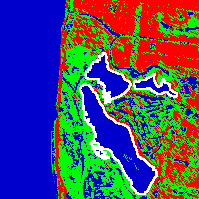
\includegraphics[width=\columnwidth]{Figures/ALOS2_SF_3Class/Lake_cl}
\caption{}
\label{fig:cla2_c}
\end{subfigure}
%\begin{subfigure}[t]{0.31\columnwidth}
%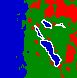
\includegraphics[width=\columnwidth]{Figures/RS2_SF_3Class/merced_cl}
%\caption{San And. Lake}
%\end{subfigure}
%\begin{subfigure}[t]{0.16\textwidth}
%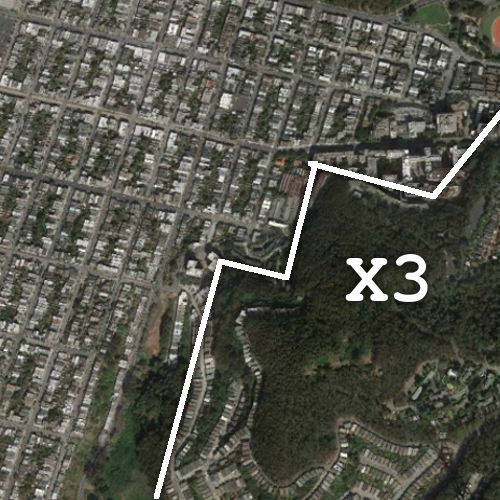
\includegraphics[width=\columnwidth]{Figures/ALOS2_SF_3Class/McLarenIm}
%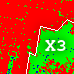
\includegraphics[width=\columnwidth]{Figures/ALOS2_SF_3Class/McLaren}
%\caption{UCSF}
%\label{fig:cl_d}
%\end{subfigure}
%\begin{subfigure}[t]{0.31\columnwidth}
%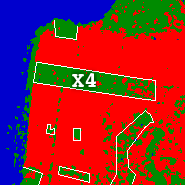
\includegraphics[width=\columnwidth]{Figures/RS2_SF_3Class/BotGard_cl}
%\caption{Sunset Blvd.}
%\end{subfigure}
\begin{subfigure}[t]{0.19\textwidth}
\includegraphics[width=\columnwidth]{Figures/ALOS2_SF_3Class/SunsetIm} 
\vspace{0.2cm}
\includegraphics[width=\columnwidth]{Figures/ALOS2_SF_3Class/Sunset}
\caption{}
\label{fig:cla2_e}
\end{subfigure}
%\begin{subfigure}[t]{0.31\columnwidth}
%\includegraphics[width=\columnwidth]{Figures/RS2_SF_3Class/OaklandPort_cl}
%\caption{Port Oakland}
%\end{subfigure}
\begin{subfigure}[t]{0.19\textwidth}
\includegraphics[width=\columnwidth]{Figures/ALOS2_SF_3Class/JettyIm} 
\vspace{0.2cm}
\includegraphics[width=\columnwidth]{Figures/ALOS2_SF_3Class/Jetty}
\caption{}
\label{fig:cla2_f}
\end{subfigure} %
%\begin{subfigure}[t]{0.31\columnwidth}
%\includegraphics[width=\columnwidth]{Figures/RS2_SF_3Class/jmpark_cl}
%\caption{Port Oakland}
%\end{subfigure} 
\caption{Crops of the classified map shown alongside corresponding aerial imagery courtesy ESRI/Bing Maps.}
\label{fig:cl_crop_alos2}
\end{figure}




\subsubsection{Analysis of Classification Performance}
\label{sec:EXPT2}
%The ALOS-2 dataset collected over San Francisco, CA is classified using the described methodology. This radar operates in the L-band ($\lambda = 24 $cm). 


%These areas however return a much stronger echo in the C-band data set, as the surface perturbations are comparable to the radar wavelength in that case causing the return to be non-specular~\cite{lee2009polarimetric}. 



The Pauli composite image generated from the dataset is shown in Figure~\ref{fig:train1alos2} along with the training areas superimposed on it. They are derived from the interpretation of aerial imagery (ESRI/Bing Maps), topographical maps (USGS) and the Pauli composite and are marked with red polygons for urban areas, green for forest/vegetation areas, and blue for water. The pixels enclosed in these polygons form the ground truth. The proportion of ground-truth pixels in each class is approximately the same, and in total, they constitute less than $\sim10\%$ of the total pixels in the image. These are randomly divided into three groups: training, test and validation. Pixels in the training set are used in the training of the network. At regular intervals within the training iterations, the process is halted and the test pixels are used to evaluate the accuracy of the network. The difference between the training and test accuracy is used to ensure that the training phase is progressing without over-fitting or memorization. To quantify the final performance of the classifier, validation pixels are employed. The confusion matrix is and is presented in Table~\ref{tab:alos2tab}.

%From these ground-truth pixels, $\frac{1}{}$ the pixels are randomly selected as training pixels, and the rest are reserved for test. A testing phase is run every 1000 iterations which measures the accuracy of prediction over this labeled set. 












\begin{table}[tbp]
	\caption{Confusion matrix and accuracy statistics for ALOS-2 San Francisco, CA dataset using the proposed supervised classification scheme incorporating textural information}
	\label{tab:alos2tab}
	\begin{tabularx}{\columnwidth}{X|XXX|X}
		& Urban & Water  & Forest & Prod. Acc. \\ \hline
		Urban & \bf{84.20} & 0 & 4.39 & 95.45  \\
		Water & 1.3 & \bf{96.86} & 3.41 & 96.00 \\
		Forest & 14.5 & 3.14 & \bf{92.20} & 84.41\\ \hline 
		User Acc. & 84.85 & 96.97 &   92.93 & \\ \hline
		OA &  91.63 \% & & &  \\
		Kappa & 0.85 & & &  \\
	\end{tabularx}
\end{table}


% Alos-2 images'
\begin{figure}[tbp]
\centering
		\includegraphics[width=0.5\columnwidth]{Figures/ALOS2_SF_3Class/Train}
		\caption{Pauli RGB image constructed from the ALOS-2 dataset collected over San Francisco, USA is shown with the ground-truth areas. The urban class is enclosed in red, the forest/vegetation in green and water in blue polygons.}
		\label{fig:train1alos2}
\end{figure}

\begin{figure}[tbp]
\centering
		\includegraphics[width=0.5\columnwidth]{Figures/SF}
		\caption{Aerial imagery collected over San Francisco, USA depicting the extent covered by the ALOS-2 dataset courtesy of ESRI/Bing Maps.}
		\label{fig:OpticalAlos2}
\end{figure}

\begin{figure}[tbp]
	
	\begin{subfigure}[t]{0.19\textwidth}
		\includegraphics[trim={150px 80px 40px 50px},clip,width=\columnwidth]{Figures/ALOS2_SF_3Class/OP_300} 
		\caption{Proposed}
		\label{fig:proposed_al2}
	\end{subfigure}
	\begin{subfigure}[t]{0.19\textwidth}
		\includegraphics[trim={150px 80px 40px 50px},clip,width=\columnwidth]{Figures/ALOS2_SF_3Class/svm_classification_file_2016_04_07_12_23_47_rbf} 
		\caption{SVM RBF}
		\label{fig:al2_svm_rbf}
	\end{subfigure}
	\begin{subfigure}[t]{0.19\textwidth}
		\includegraphics[trim={150px 80px 40px 50px},clip,width=\columnwidth]{Figures/ALOS2_SF_3Class/svm_classification_file_2016_04_07_12_20_26_lin} 
		\caption{SVM Polynomial}
		\label{fig:al2_svm_poly}
	\end{subfigure}
	\begin{subfigure}[t]{0.19\textwidth}
		\includegraphics[trim={150px 80px 40px 50px},clip,width=\columnwidth]{Figures/ALOS2_SF_3Class/wishart_supervised_class_1x1_poc} 
		\caption{Wishart with POC}
		\label{fig:al2_wish_1_poc}
	\end{subfigure}
	\begin{subfigure}[t]{0.19\textwidth}
		\includegraphics[trim={150px 80px 40px 50px},clip,width=\columnwidth]{Figures/ALOS2_SF_3Class/wishart_supervised_class_1x1} 
		\caption{Wishart}
		\label{fig:al2_wish_1}
	\end{subfigure}
	\caption{Comparison of common classification techniques with the proposed method.}
	\label{fig:comparison_al2}
\end{figure}

The dataset is classified with an overall accuracy of $91.63\%$ and a Kappa coefficient of 0.85. Urban areas are classified with an accuracy of $84.2\%$. The urban class is mostly confused with the forest class. This is primarily due to the fact that both, urban areas rotated with respect to the radar line of sight and vegetation have higher cross-polarized return. Certain small, smooth vegetated areas like parks. have been misclassified as the water class, contributing to the error of $3.14\%$ due to the low backscattered power as  previously highlighted. 

The resultant  map is presented in~Figure~\ref{fig:compwal2}. Reference aerial photographs are given in Figure~\ref{fig:OpticalAlos2}. We can see a close correspondence between the areas that appear to be urban in the optical aerial images and the  classification result. %This is unlike the Pauli composite image where the urban a[]reas behave like vegetation.
Detail subsets from selected areas of the classification output along with the corresponding aerial imagery, representing the ground truth, are shown in Figure~\ref{fig:cl_crop_alos2}. This demonstrates the performance of the proposed algorithm on the considered dataset. The resolution of this imagery is $\sim0.3m$ and is significantly higher than that of the classified map. However, reasonable correspondence can be seen between the two. 



%Detail crops of the classified output from the proposed method is shown in Figure~\ref{fig:cl_crop_alos2} along side aerial imagery of the same area. 
%The resolution of the the aerial is about $\sim$0.3m whichis more  comparable to the 6m effective resolution of ALOS-2 than the RadarSAT-2 dataset. 


The subset shown in Figure~\ref{fig:cla2_a} represents a dense urban area that is oriented at an angle $\sim-20^\circ$ from the radar line of sight, marked as Area `A1' in the image. Due to this large orientation, this region is often misclassified~\cite{lee11_5491157}, however it is classified correctly using the proposed method. %The proposed method involves the synthetic rotation of the data which is then given as input to the first auto-encoder stage. This causes a generalized target representation to be learned by the structure. We extract features from the auto-encoder which is representative of the response from the target and its possible orientations. In the third stage the MLP classifier is able to leverage this additional information to successfully classify this area. The auto-encoder stage is thus able to incorporate the additional information from the  synthetic rotated datasets into the classification scheme. 
% ~\cite{zhang2011extraction} bridge 
The subset shown in Figure~\ref{fig:cla2_b} shows the Golden Gate bridge, marked as `A2' and some surrounding areas. Apart from the return from the bridge itself,   multi-path returns from reflections from the bridge and the water surface can also be seen. The radar echoes from the vicinity of the bridge are quite strong and have a high value of $\gamma^0$. This causes the third stage of the classifier, which takes $\gamma^0$ as an input, to classify this pixels immediately under the bridge as forest. 
Figure~\ref{fig:cla2_c} shows a lake surrounded by urban and vegetated areas. This is marked with a white outline on the aerial images and classification maps.  It can be seen that the lake  is well discriminated from other classes. As discussed earlier, the smooth vegetated surfaces near the lake are misclassified as water due to near specular reflection at L-band frequencies and low incidence angles. 

The area marked as `A3' in the subset shown in Figure~\ref{fig:cla2_e} consists of a park between two regions of high density urban areas. It can be seen that the area of vegetation is well identified. The high resolution of ALOS-2 allows the faithful classification of small features in this park as well.  To further exploit high resolution datasets like ALOS-2 for classification of fine details, it is possible to avoid filtering operations in the SAR pre-processing step. Since, the proposed technique is pixel based, it does not cause a degradation in resolution.  
% Since the proposed technique does not require a window based processing, it is able to take advantage of the high spatial resolution of the ALOS-2 dataset. 
Subset shown in Figure~\ref{fig:cla2_f} is of a jetty. The white arrow marks a pier structure which has interleaving perpendicular cylindrical masts. This shows a high double bounce return which does not reduce with rotation of the target about the radar line of sight. This enables the classifier to correctly identify this structure. %The floor of the pier is made of wood and asphalt and is classified into the non-urban class. 

% % % % % % % % % % % % % % % % % % % % % % % % % % % % % % % %
%The methodology is also applied to a RADARSAT-2 C-band dataset and similar results are obtained (Figure~\ref{fig:RSAT}). The resolution of the dataset is slightly lower, thus it is not possible to discern individual building and road structure as seen in the ALOS-2 results, however the classification output is satisfactory and the developed technique is not limited by sensing frequency. 






% % RSAT
%\begin{figure}[!htb]
%		\centering
%	\begin{subfigure}[t]{0.45\columnwidth}
%	\includegraphics[width=\columnwidth]{Figures/RS2_SF_3Class/TrainingAreasCrop.png}
%		\label{fig:output}
%		\caption{Training areas}
%	\end{subfigure}
%	~
%	\begin{subfigure}[t]{0.45\columnwidth}
%	\includegraphics[width=\columnwidth]{Figures/RS2_SF_3Class/OUTPUT_3x3_CROP.png} 
%	\label{fig:output1}
%	\caption{Classification Map}
%	\end{subfigure}
%%	~	
%	\begin{subfigure}[b]{\columnwidth}
%	\centering
%	\begin{tabular}{clclcl}
%				\includegraphics[width=0.015\columnwidth]{Figures/RS2_SF_3Class/Blue.png} & Water &		\includegraphics[width=0.015\columnwidth]{Figures/RS2_SF_3Class/Green.png} & Forest &  	\includegraphics[width=0.015\columnwidth]{Figures/RS2_SF_3Class/Red.png} &  Urban 
%	\end{tabular}
%	\end{subfigure}
%
%\caption{Classified map of San Francisco derived from an RADARSAT-2 full polarimeteric C-Band dataset acquired on 9 April 2009 if FQ-2 mode. }
%		\label{fig:RSAT}
%\end{figure}
%



%%%%%%%%%%%%%%%%%%%%%%%%%%%%%%%%%%%%%%%%%%%%%%%%%%%%%%%
\subsubsection{Analysis of the Learned Representation}
\label{sec:EXPT3}
%Analysis of the Auto-Encoder Action

\begin{figure}[tbp]
	\centering
	\includegraphics[width=0.85\columnwidth]{Figures/Wr_decode3_11_g}
	\\
	\includegraphics[width = 0.3\columnwidth]{Figures/Rotation_FS/GRAY}
	\caption{Extracted feature map for one of the internal nodes in the representation layer from the trained AE.}
	\label{fig:wr}
\end{figure}

To understand the information encoded in the representational layer of the AE, the response of one of the nodes it is extracted and shown in  Figure~\ref{fig:wr} after the completion of the training phase. This is one of the many internal representations encoded by the network. Since the network is initialized randomly, the exact position of the internal node containing information and its encoding will change each time the network is trained. However, in general, it is observed that each internal node learns a different encoding of the data-set. 
The representation is sparse in nature with only small percentage of nodes containing useful information for classification. 
Area `A4' consists of urban areas both perpendicular to and oriented away from the radar line of sight. Although they appear distinct in the Pauli visualization (Figure~\ref{fig:train1alos2}), the trained network evokes a uniformly strong response from the area. Thus the AE is able to combine the information from the synthetically rotated urban target database to form an internal representation that is independent of the target orientation. This allows for the accurate classification of the urban areas. In contrast, homogeneous areas like Area `A5' have a lower response allowing them to be distinguished  in the final classification.  
	%- one of the many internal representations
	%- each representation learns a different encoding
	%- sparse repn with only some features having useful data
	%- we see that in area A - urban - irrespective of the orientation the network has a strong response 
	%- in contrast in area B lower response.
	%- this property of the NN allows it to classify



\subsubsection{Comparison with State of the Art Classifiers}
\label{sec:EXPT4}


\begin{table}[tbp]
\centering

\caption{Class-by-class test-area accuracy statistics for ALOS-2, San Francisco, CA dataset for the proposed technique, SVM with RBF kernel, the SVM with Polynomial kernel and the Wishart supervised classifiers. }
\label{tab:alos_comparison} 
\begin{tabularx}{\columnwidth}{X|XXXXX} 
 & Proposed & SVM-RBF  & SVM-Poly & Wishart + POC& Wishart  \\ \hline
Urban & 86.2 & 64.2 & 58.5 & 59.1 & 55.6 \\
Water & 98.1 & 96.4 & 96.3 & 92.1 & 92.1 \\
Forest & 86.1 & 84.2 & 83.6 & 83.2 & 82.8 \\ \hline
OA & 90.8  & 81.6 & 79.4 & 78.14 & 76.83  \\ 
\end{tabularx}
\end{table}

The proposed method is compared with other commonly used SAR classification techniques. The same training areas were used to train all classifiers.
%The ALOS-2 dataset collected over San Francisco has been classified using the proposed method, 
%the Wishart supervised classifier, and SVM classifiers with a polynomial and radial basis function (RBF) based kernel. 
%The same training areas were used to train all classifiers. 
%A crop of the results are presented in Figure~\ref{fig:comparison_al2}. The areas shown in the crop, marked `A' and `B', are highly urbanized as seen in the optical image collected over the area shown in~Figure~\ref{fig:OpticalAlos2}. However, it is only classified successfully the proposed method. The other  methods misclassify it as forest/vegetation because of its significant orientation. %The cross-polarized return from the area makes it difficult to discern this from actual areas of vegetation. However, due to the synthetic rotation the proposed scheme is able to account for this orientation information and more successfully classify the data, while maintaining high textural fidelity. 


The class-by-class accuracy is reported in Table~\ref{tab:alos_comparison} and the results are presented in Figure~\ref{fig:comparison_al2}. The SVM classifier was run with two kernels: a polynomial kernel (SVM-Poly) and a RBF kernel (SVM-RBF). The parameters of the RBF kernel were determined by the method described in~\cite{liu2011gaussian}. The polynomial kernel used has a degree of 4. The Wishart classifier was run both with Polarization Orientation Correction  (Wishart+POC) and without (Wishart). The proposed classifier has an urban area classification accuracy of 86.2\%. It outperforms the SVM-RBF, SVM-Poly Wishart+POC and Wishart classifier which have urban area accuracies of 64.2\%, 58.2\%, 59.1\% and 55.6\% respectively. The POC is able to improve the discernibility. However, targets that are oriented significantly with respect to the radar line of sight are still misclassified. 

The areas shown in the subset, marked `A' and `B', are highly urbanized as seen in the optical image collected over San Francisco (Figure~\ref{fig:OpticalAlos2}).
The cross-polarized return from area `A' makes it difficult to discern this from actual areas of vegetation. However, due to the synthetic rotation the proposed scheme is able to account for the orientation information and more successfully classify the region than the other methods, while maintaining high textural fidelity. 
%On qualitative examination of the classified images, we find that the proposed method has the best performance. 
%It is able to classify more regions of area `A' correctly, followed by the SVM-RBF classifier. 
The mean orientation angle of area `B' is almost perpendicular to that of area `A', and the region is characterized by large open spaces between man-made structures. The mixed nature of the pixels makes classification more difficult. As seen in Figure~\ref{fig:proposed_al2}, the proposed technique correctly classifies these structures while largely preserving the texture. The other methods erroneously classify most of this region with the RBF kernel SVM performing  better than the polynomial kernel SVM and Wishart supervised classifier. Wishart+POC performs slightly better than SVM with the polynomial kernel.

 % OK



\chapter{Semi-supervised Change Detection}

In this chapter, a novel methodology for semi-supervised classification of changes in urban built-up areas in PolSAR images is proposed (Section~\ref{sec:sfo_ba145}). Further, experiments are conducted to test and validate this methodology (Section~\ref{sec:exp}). Finally, the results of the experiments are discussed (Section~\ref{sec:resultsA1}). 

\section{Methodology} 
\label{sec:sfo_ba145}
\begin{figure}[tbhp]
\centering
\includegraphics[width=\textwidth]{Figures/CD/BLOCK}
\caption{Block scheme of proposed methodology.}
\label{fig:1_method}
\end{figure}

% % % % Removing the headers
% \section{Proposed DNN based Framework}
\label{sec:Method}
In disaster relief and urban monitoring, typically CD analysis is applied in order to highlight the changed urban areas. On the other hand, a further analysis discriminating the unchanged urban areas from natural ones is desirable. Additionally, multi-temporal ground campaigns are often difficult and very few ground truth points may be available.   
%For disaster relief and urban monitoring operations, it is desirable to obtain simultaneous change and land-cover maps using very few training samples. 
The motivation behind this study is to develop a framework that can simultaneously perform accurate urban change detection and land-cover classification in a weakly supervised manner. The framework takes multi-temporal polarimetric SAR images as input and produces an output with 3 classes: changed urban areas, unchanged urban and unchanged natural areas. This kind of maps are useful for urban monitoring and rescue operations. %The two unchanged classes are also grouped to produce a binary urban change map. 

The  block scheme of the proposed methodology is shown in Figure~\ref{fig:1_method}. Two PolSAR images  acquired over the same geographic area at time instants $t_0$ and $t_1$,  are pre-processed and normalized  (Section~\ref{sub:pre})  before being given as input to a Stacked Auto-Encoder (AE) network (Section~\ref{sub:ae}). The AE is trained in an unsupervised manner to create an optimal representation, assuming that only a very small amount of ground truth is available, a label aggregation step is undertaken before classification by a Multi-layer Perceptorn (MLP) (Section~\ref{sub:weak}). 
The use of a AE with stacked features has the advantage of preserving both change and multi-temporal polarimetric scattering information which is exploited by the final classifier. % % DELETEABLE

%Muller matrices are derived from the data collected at time $t_0$ and $t_1$ .... parcel.... normalized in the range $[0,1]$ such that the histogram of the original data is preserved. This is simultaneously applied to the input of an stacked de-noised AE. The AE learns a representation that is able to maximally separate the changed areas from the unchanged areas. Since this representation also contains polarimetric information from both the Mueller matrices, in addition to identification of changed ares, it also is possible to classify the unchanged land-cover. 

%motivation
\begin{figure}[tbhp]
\centering
\includegraphics[width=0.6\columnwidth]{Figures/CD/SAE}
\caption{Block diagram of the unsupervised Stacked AE stage.}
\label{fig:SAE}
\end{figure}

\subsection{Data Preprocessing}
\label{sub:pre}
The full PolSAR complex backscattering matrix $\mathbf{S}$ consists of four independent measurements (HH, HV, VH and VV) with the phase relations preserved and is expressed as,
\begin{equation}
\mathbf{[S]} =
  \begin{bmatrix}
    S_{hh} & S_{hv}  \\
    S_{vh} & S_{vv}
  \end{bmatrix}
 \label{eqn:scattring}
\end{equation}
This can be expressed as Mueller matrix $\mathbf{M}$ as follows, 
\begin{equation}
\mathbf{M} = \mathbf{A}^* \left( \mathbf{S} \otimes \mathbf{S^{*}} \right) \mathbf{A^{-1}} 
\end{equation}
where,
\begin{equation} \small
\mathbf{A} = \begin{bmatrix}
    1 & 0 &  0 & 1 \\
    1 & 0 & 0&  -1\\ 
    0 & 1 &  1  &  0 \\
    0 & j  & -j & 0 \\
\end{bmatrix}
\end{equation}
Although when expressed in the backscatter convention, the matrix is named Kennaugh $\mathbf{K}$, it is common practice in literature to refer to it uniformly as $\mathbf{M}$. 

The $\mathbf{M}$ representation is constructed for images at $t_0$ and $t_1$.
Since SAR images are affected by speckle~\cite{lee1994speckle}, it is desirable to perform a smoothing or suppression step to reduce false alarms. A super-pixel (SP) based filtering technique is used. Simple Linear Iterative Clustering (SLIC) algorithm~\cite{6205760} with a perturbation window $n_w$ is applied on the Pauli composite of image acquired at $t_0$ to form super-pixels (SPs).  $\mathbf{M}$ is  averaged over SPs for both the $t_0$ and $t_1$ images to reduce the effect of speckle on the  change detection performance, This approach yields high edge preservation while providing maximum smoothing over homogeneous areas. 
The dynamic range of the dataset is  jointly normalized in the range $[0,1]$ for faster convergence of the optimization solver algorithm and  for efficient training of the network. 
%The Simple Linear Iterative Clustering (SLIC) algorithm~\cite{6205760} with a perturbation window $n_w$ is applied on the Pauli composite of image at $t_0$ to form super-pixels (SPs). The $\mathbf{M}$ is then averaged over these SPs for both the $t_0$ and $t_1$ images to reduce the effect of speckle on the final change detection performance. This approach yields high edge preservation while providing maximum smoothing over homogeneous areas. This characteristic is desirable for training the AE. 
  %SLIC
 
%\subsection{Superpixel}
%Since SAR images are affected by speckle~\cite{lee1994speckle}, it is desirable to perform a smoothing or suppression step to reduce false alarms. An adaptive window based  based on the SLIC algorithm~\cite{6205760} with a perturbation window $n_w$ is applied on the Pauli composite of image at $t_0$. The $\mathbf{M}$ is then averaged over this windows  for both the $t_0$ and $t_1$ images. 

%\subsection{Normalization}
%The $\mathbf{M}$ representation is real valued allowing 


% SLIC? 
%\subsubsection{Unsupervised Representation Learning using a Stacked Auto-Encoder Network}
\subsection{Unsupervised Representation Learning using Auto-Encoders}
\label{sub:ae}

The pre-processed $\mathbf{M}$ elements from the image pair for each corresponding pixel is stacked together  to form the input vector $x$, which is given to stacked AE (Figure~\ref{fig:SAE}). The objective of the AE is to reconstruct output $x'$ to match $x$ as closely as possible. The loss function of the AE is modified to be a combination of L2 norm and Cross Entropy error given by,

\begin{dmath} 
E = \lambda_{w1} \frac{-1}{N}\sum_{n=1}^{N}[x_n \log \hat{x_n} + (1 - x_n)\log(1-\hat{x_n})] 
     + \lambda_{w2} \frac 1 {2N} \sum_{i=1}^N \| x^1_i - x^2_i \|_2^2
\end{dmath}

where $\lambda_{w1},\lambda_{w2},$ are the loss weighting parameters, $N$ is the total number of samples in the dataset and $E$ is the total loss evaluated for back-propagation. This modified loss function leads to a representation that maximally separates changed from unchanged areas. Further to prevent over fitting, a weight decay strategy is applied with the regularization term $\lambda \sum_{i=0}^{|N|} (x_i-x'_i)^2$, where $\lambda$ is the decay parameter. Since $|N|$ is quite large for the complete dataset, the optimization is performed in smaller mini-batches of $D << |N|$. Regularization constrains the AE to be less sensitive to the input, but in minimization of the reconstruction error, it remains sensitive to variations along the manifold of high density. %~\cite{bengio2013representation}.  

%\subsection{PCA}
After  training, the representational layer $z$ is extracted as a feature from the AE. Principle Component Analysis (PCA) is applied to transform $z$  to a set of linearly uncorrelated variables $PC_1, PC_2... PC_n$ by projection into the eigenvector space. The information content in each $PC$ is evaluated by ordering the set of eigenvalues and considering the corresponding top $k$ $PCs$ for label aggregation. 

\begin{figure}[tbhp]
\centering
\includegraphics[width=0.8\columnwidth]{Figures/CD/3d}
\caption{Mechanism of MVBE fitting for labeled sample generation in the PC space.}
\label{fig:MVE}
\end{figure}

%\subsubsection{Weakly Supervised Classification using Feed Forward Network}
\subsection{Weakly Supervised Classification}
\label{sub:weak}
Ground reference labels are assumed to be available for only a small portion of the scene. This is a realistic assumption for disaster relief or monitoring efforts, where information would be available at a point of the scene where administrative efforts are concentrated. However the total number of labeled pixels  is $l << N$ and hence the framework is said to be weakly supervised. The use of very few samples  will lead to poor accuracies as the dataset is under-represented. Thus a label aggregation step is performed. In the $PC_k$ space a convex-hull is fitted for each class on the labeled samples, in order to reduce the number of considered points and simplify computation. Then a minimum volume bounding ellipsoid (MVBE) is fitted on these points as illustrated in Figure~\ref{fig:MVE}. Thinning along the radial axis of the ellipsoid is performed to exclude points that lie on the periphery of the volume, having a lower probability of belonging to the class than a more internal point. After thinning, points that lie within each ellipsoid are assumed to belong to the corresponding class and are preselected for labeling. From these, an equal number of samples $L$ are chosen per-class using the reservoir sampling technique to preserve the distribution of each class. These  samples are then to assigned the corresponding class labels, increasing the number of labeled samples available to the final classifier.  
% % EQUATIONs And figures
A Multi-Layer Perceptron (MLP) network is used to perform the final classification with the aggregated labels. The extracted representation $z$ is used in the classification with the aggregated labels to produce the final output map. %This represents both the changed urban areas and a land-cover classification of the unchanged areas: simultaneously generating an urban change and extent map.








 % OK

%% Crop classification methodology


\section{Dataset and Study Area}

A pair of co-registered L-band ($\lambda = 0.23m$) UAVSAR images acquired over Los Angeles, California in 23-04-2009 and 11-05-2015 respectively  with a resolution of $0.4m$ in azimuth and $1.66m$ in range are used in this study. The dataset is multi-looked $2\times8$ times to form an effective pixel-size of $3.2m$.  The study-area is a dense urban area with changes occurring primarily due to the effects of urbanization. 

The objective of the proposed methodology is to  characterize the construction and destruction of urban areas, while simultaneously classifying unchanged urban and natural areas in the rest of the scene.
The major changes, i.e. `Changed Urban' class observed include the construction of suburban neighborhoods, industrial structures and public infrastructure like rail-yards and airports.  Natural areas of vegetation  comprise of the `Natural Unchanged' class. The urban infrastructure like houses, buildings, roads etc. that did not change is the 'Urban Unchanged' class.
%Thus the classes "Changed Urban" This represents both the changed urban areas and a land-cover classification of the unchanged areas: simultaneously generating an urban change and extent map.

%\section{Experimental Results and Discussion}
\section{Experimental Set-Up}
\label{sec:exp}
The images are pre-processed and stacked to form the 20 dimensional input vector $x$.  The AE is a sparse 7-layer network comprised of 512, 256, 128 nodes in the encoder, 8 in the representational layer and 128, 256, 512 in the decoder with ReLU nodes. The auto-encoder is trained in an unsupervised manner with learning rate $\alpha=1e-5$ at initialization and is dropped by a step factor of $\Gamma=0.1$ every $100,000$ iterations.  After training,  $z$ is extracted from the representational layer and a PCA is applied pixel wise. It is seen that $k=3$ principal components contain most of the useful information.
% activation function used is ReLU. The learning rate $\alpha=1e-5$ at initialization and is dropped by a step factor of $\Gamma=0.1$ every $100,000$ iterations.

\begin{figure}
\centering
\includegraphics[width = 0.7\textwidth]{Figures/CD/ADD/plot}
\caption{Map of all the ground reference information used for CD. As can be seen, the reference information is minimal, and constrained to a small spatial area of the scene.}
\label{fig:const}
\end{figure}

In a realistic scenario, reference information about the scene would only be available in a small portion of the area. Hence training samples are drawn from the part of the scene bounded by the yellow square in Figure~\ref{fig:2_a}. For each class $20$ pixels are labeled based on prior knowledge of the region and optical imagery as shown in Figure~\ref{fig:const}. A total of $l=60$ training samples are  used, and $l<<N=9e6$ making the problem weakly supervised. A label aggregation step is performed by the ellipsoidal fitting technique described above. Reservoir sampling is performed to select $L=300$ labeled pixels per class from the points bounded by each ellipsoid. These aggregated labels are used to train a 3-layer MLP network with sigmoid activation function in a supervised manner. The final classification output   is shown in Figure~\ref{fig:2} along with the Pauli composition of the image pair. The output simultaneously maps areas of changed urban ares, unchanged built-up and  natural land-cover. This is an improvement over outputs from  traditional ratio based methods that are unable to leverage the polarimetric information. 

\section{Results and Discussion}
\label{sec:resultsA1}

\begin{figure}[tbp]
\centering
\begin{subfigure}[b]{0.32\textwidth}
		\includegraphics[width=\textwidth]{Figures/CD/2009}
		\caption{}
		\label{fig:2_a}
\end{subfigure}
\hspace{0.05pt}
\begin{subfigure}[b]{0.32\textwidth}
		\includegraphics[width=\textwidth]{Figures/CD/2015.jpg}
		\caption{}
		\label{fig:2_b}
\end{subfigure}
\hspace{0.05pt}
\begin{subfigure}[b]{0.32\textwidth}
		\includegraphics[width=\textwidth]{Figures/CD/result}
		\caption{}
		\label{fig:2_c}
\end{subfigure}

%\hspace{0.05pt}
\begin{subfigure}[b]{\textwidth}
\centering
		\vspace{0.2em}
		\begin{tabular}{ c l  c l  c l  }
	%	\hline
		 \includegraphics[width=0.01\columnwidth]{Figures/CD/RED} & Urban Change (UC)  \hspace{1mm} &
		 \includegraphics[width=0.01\columnwidth]{Figures/CD/GREEN} & Natural Unchanged (NU) \hspace{1mm} &
		 \includegraphics[width=0.01\columnwidth]{Figures/CD/BLUE} & Urban Unchanged (UU) \hspace{1mm} \\
	%	\hline
		\end{tabular}
		%\vspace{20mm}
		%\caption{}
\end{subfigure}
\caption{The Pauli composite of (a) 2009, (b) 2015 image, and (c) the result of the classification. }
\label{fig:2}
\end{figure}



\begin{figure}[tbp]
\centering
\begin{subfigure}[b]{0.7\textwidth}
		\includegraphics[width=\textwidth]{Figures/CD/ADD/1}
		\caption{}
\end{subfigure}

\begin{subfigure}[b]{0.7\textwidth}
		\includegraphics[width=\textwidth]{Figures/CD/ADD/2}
		\caption{}
\end{subfigure}

\begin{subfigure}[b]{0.7\textwidth}
		\includegraphics[width=\textwidth]{Figures/CD/ADD/3}
		\caption{}
\end{subfigure}

%\hspace{0.05pt}
\begin{subfigure}[b]{\textwidth}
\centering
		\vspace{0.2em}
		\begin{tabular}{ c l  c l  c l  }
	%	\hline
		 \includegraphics[width=0.01\columnwidth]{Figures/CD/RED} & Urban Change (UC)  \hspace{1mm} &
		 \includegraphics[width=0.01\columnwidth]{Figures/CD/GREEN} & Natural Unchanged (NU) \hspace{1mm} &
		 \includegraphics[width=0.01\columnwidth]{Figures/CD/BLUE} & Urban Unchanged (UU) \hspace{1mm} \\
	%	\hline
		\end{tabular}
		%\vspace{20mm}
		%\caption{}
\end{subfigure}

\caption{From left to right, the Pauli composite of the 2009 and 2015 images, along with the result of the classification is presented for areas (a) A, (b) B and (c) C. }
\label{fig:detail}
\end{figure}


\begin{figure}[t]
\centering
\begin{subfigure}[b]{0.23\columnwidth}
		\includegraphics[width=\textwidth]{Figures/CD/A2_2009}
		\caption{}
		\label{fig:3_a}
\end{subfigure}
\hspace{0.01pt}
\begin{subfigure}[b]{0.23\columnwidth}
		\includegraphics[width=\textwidth]{Figures/CD/A2_2015}
		\caption{}
		\label{fig:3_b}
\end{subfigure}
\hspace{0.01pt}
\begin{subfigure}[b]{0.23\columnwidth}
		\includegraphics[width=\textwidth]{Figures/CD/REF_A2}
		\caption{}
		\label{fig:3_c}
\end{subfigure}
\hspace{0.01pt}
\begin{subfigure}[b]{0.23\columnwidth}
		\includegraphics[width=\textwidth]{Figures/CD/OP_1_A2}
		\caption{}
		\label{fig:3_c}
\end{subfigure}

\begin{subfigure}[b]{\columnwidth}
\centering
		\vspace{0.2em}
		\begin{tabular}{c l  c l  }
		 \includegraphics[width=0.02\columnwidth]{Figures/CD/BLK} & No Change   &
		 \includegraphics[width=0.02\columnwidth]{Figures/CD/WHT} & Change
		\end{tabular}
\end{subfigure}
\caption{The Pauli composite of detail (a) 2009, (b) 2015 image, and the (c) reference change map, and (d) output change map.}
\label{fig:3}
\end{figure}



Qualitatively, the  output corresponds well with the changed areas observed in the Pauli composition image pair and has low misclassification as shown in Figure~\ref{fig:2}. Comparative crops are shown in Figure~\ref{fig:detail} for three areas of the image. Area 'A' is located close the near range of the radar, and hence is subject to radiometric anomalies due to the steep look angle of the radar, as common with airborne sensors. Despite this, the proposed method performs reasonably well and resilient to the amplitude gradient of the backscatter. The changes in area 'B' are very minor compared to the rest of the area. There is a construction of new housing that has occurred in the vacant lot amidst other built-up areas. The challenge in this crop is that it is close to a train station (right edge), and due to the movement of infrastructure there is inconsistent radar backscatter between the two images. The proposed method is able to capture the change perfectly, ignoring the interference from the railway station. Area 'C' radar artifacts due to return from power-lines can be observed in the two images. Also, the natural areas surrounding the urban structures are significantly changed. The parcel based approach employed in the proposed methodology is able to counter the effects of the artifacts. The method is also able to segregate urban changes from natural ones, something that would not be possible with a traditional change index methodology.     

Quantitatively, 
the confusion matrix is computed and presented in Table~\ref{tab:conf}.  The overall accuracy $OA = 92.34\%$ with $\kappa = 0.88$. The urban change (UC) areas are most commonly confused with the urban unchanged (UU) ones. This corresponds to areas where the learned representation was not sufficient to discriminate the two.
Another source of confusion is between natural unchanged (NU) and UU classes. The presence of vegetation intermixed with buildings in the UU areas makes it more difficult to discern it from the NU class leading to misclassification.
%The Pauli composition of the two images are shown in Figure~\ref{fig:3} with the 






To evaluate the CD capabilities the two unchanged classes, i.e. UU and NU are grouped together as a single unchanged class, with the UC representing the change as shown in Figure~\ref{fig:3}. Performance is evaluated in terms of false positive rate (PFP), false negative rate (PFN), false alarm rate (FA(\%)), detection rate (DR(\%)) and kappa (Table~\ref{tab:cd}). The method has a low FA rate of $FA=2.64\%$. This is due to design of the AE loss function and the radial thinning performed in the label aggregation step. The $DR=82.3\%$ can be improved at the cost of a higher $FA$, by eliminating the radial thinning step during label aggregation. The $\kappa=0.83$ indicates that there is very good agreement between the reference and output maps. This is confirmed qualitatively by visual inspection of the output image. 


\begin{figure}[t]
\centering
\includegraphics[width = 0.6\textwidth]{Figures/CD/ADD/Diff}
\caption{A traditional log-ratio change index generated for the dataset.}
\label{fig:difflr}
\end{figure}


Figure~\ref{fig:difflr} depicts a traditional log-ratio change index computed on the dataset. The index can reasonably capture the change in the scene, but the original scattering mechanism information is discarded. This prevents simultaneous land-cover classification from being performed. To obtain both the change and land-cover map, two separate processes must be run on the dataset consuming time and computing resources. In contrast, the proposed method is able to efficiently compute both the maps in one go. 

Further, the change index is unable to differentiate between natural and urban changes and only captures the magnitude of the change, disregarding scattering information. Thus, it identifies both the natural and urban changes in the scene as a change, and further analysis is needed to be able to identify the change. In the proposed method, the changes are encoded in the representational layers of the AE, which is then projected in a manifold. Because the scattering information is encoded inherently in this representation, each region of the space corresponds to a particular transition of scattering mechanism between the two images. Due to this it is possible to not only identify the original land cover classes, but also the change information in one step. In a work-flow where a large number of scenes must be automatically processed, this computational advantage can translate to time and resource savings.

\begin{table}
	\centering
	\caption{Confusion Matrix}
	\label{tab:conf}
	\begin{tabular}{cccc|c}
		&  UC (\%)  & NU (\%) & UU (\%) & Total \\ \hline
		UC (\%) & 90.28 & 0.34 &  0.00 & 26.11 \\
		NU (\%) & 2.24 & 88.54 & 1.10  & 35.91\\
		UU (\%) & 7.47 & 11.12 & 98.90 & 37.97\\ \hline
		OA   & 92.34\% &  $\kappa$   & 0.88 & \\ 
	\end{tabular}
	
\end{table}
\begin{table}
	\centering
	\caption{Change Detection Metrics}
	\label{tab:cd}
	\begin{tabular}{c c c c c c}
		PFP(\%)  & PFN(\%) & FA(\%) & DR(\%) & $\kappa$ \\ \hline
		0.89 & 1.75 & 2.64 & 82.3 & 0.83 \\
	\end{tabular}
\end{table}



\subsubsection{Comparative Analysis}

\begin{figure}[t]
\centering
\begin{subfigure}[b]{0.18\columnwidth}
		\includegraphics[width=\textwidth]{Figures/CD/ADD/a}
		\caption{}
\end{subfigure}
\hspace{0.01pt}
\begin{subfigure}[b]{0.18\columnwidth}
		\includegraphics[width=\textwidth]{Figures/CD/ADD/b}
		\caption{}
\end{subfigure}
\hspace{0.01pt}
\begin{subfigure}[b]{0.18\columnwidth}
		\includegraphics[width=\textwidth]{Figures/CD/ADD/c}
		\caption{}
\end{subfigure}
\hspace{0.01pt}
\begin{subfigure}[b]{0.18\columnwidth}
		\includegraphics[width=\textwidth]{Figures/CD/ADD/d}
		\caption{}
\end{subfigure}
\hspace{0.01pt}
\begin{subfigure}[b]{0.18\columnwidth}
		\includegraphics[width=\textwidth]{Figures/CD/ADD/e}
		\caption{}
\end{subfigure}

\begin{subfigure}[b]{\columnwidth}
\centering
		\vspace{0.2em}
		\begin{tabular}{c l  c l  }
		 \includegraphics[width=0.02\columnwidth]{Figures/CD/BLK} & No Change   &
		 \includegraphics[width=0.02\columnwidth]{Figures/CD/WHT} & Change
		\end{tabular}
\end{subfigure}
\caption{The Pauli composite of detail (a) 2009, (b) 2015 image, and the result of change detection by (c) proposed and (d) geodesic distance methods, shown along with the (e) reference map.}
\label{fig:comparedeb}
\end{figure}

\begin{table}[]
\centering
\caption{Comparison with other methods}
\label{tab:comparedebanshu}
\begin{tabular}{l|llll}
Approach             & Overall Accuracy & Kappa &  &  \\ \hline
Geodesic Distance (GD)~\cite{ratha2017change}    & 89.20            & 0.78  &  &  \\
Proposed             & 92.34            & 0.88  &  & 
\end{tabular}
\end{table}

The proposed methodology is compared with another recent PolSAR change detection technique~\cite{ratha2017change}. The results are tabulated in Table~\ref{tab:comparedebanshu} and shown in Figure~\ref{fig:comparedeb}. The proposed method is able to outperform the contemporary technique, with an overall accuracy of $92.34\%$ and $\kappa=0.88$. The section of image used in the comparison is fairly challenging for a change detection algorithm due to the presence of power-lines in the scene. These have a very strong radar return, saturating the receiver and leading the artifacts in the image, as seen. Since both the algorithms use variation in the scattering mechanism to identify changes, they are able to successfully avoid the interference of these power-lines. In contrast, change index and amplitude difference based techniques would be susceptible to this nature of interference. 

However, the geodesic distance (GD) measure is still sensitive to changes in natural areas. Over time, vegetation will grow and change, leading to a variation in the observed scattering mechanism. Since the final output is obtained by applying a single threshold to the GD value, it is not possible to fully separate the natural changes from urban ones. In contrast, the proposed method uses ellipsoid fitting to improve the separation of urban changes in the feature space itself. This is followed by a MLP layer, which is further able to flexibly threshold the images to reduce the effect of natural changes. 
%
The region growing in the feature space and parcel based approach at input, combined lead to a very low false alarm rate of $2.64\%$ in the proposed technique, and often in practical application of change detection, a lower false alarm rate is more critical than a high accuracy. 

It must be noted that although the proposed technique outperforms the GD method, it is much more computationally complex. The training phase of the AE is also time consumptive, however, once trained, the final classification can be performed fast. In contrast, the GD method is computationally simple, and can be computed much quicker, at the cost of a slightly lower accuracy and higher false alarm rate. 

%[[156301   1001]
% [  2844  10854]]
%[[ 0.99363644  0.00636356]
% [ 0.20762155  0.79237845]]
%Overall accuracy:
%97.7514619883
%Kappa:
%0.83744617901 % OK


\chapter{Multi-frequency Crop Classification}

In this chapter, a novel tensor product and neural network based framework for classification of vegetative areas like agricultural fields and forests is presented (Section~\ref{sec:sfo_ba33}). Further, experiments are conducted to test and validate the proposed methodology (Section~\ref{sec:delta_911}). Finally, the results of the experiments are discussed (Section~\ref{sec:jameson}). 

\section{Methodology} 
\label{sec:sfo_ba33}
% % % % header removed
%\section{Methodology}


The methodology is divided into two components: Synthesis of the feature vector using tensorization (Section~\ref{sec:tensor}) and classification using an ANN (Section~\ref{sec:ANN}). 
%\subsection{Tensorization Framework for Combination of Multi-frequency Data}
\subsection{Data Preprocessing}
\label{sec:tensor}
A tensorization framework is proposed which utilizes the Kronecker product of two matrices $\mathbf{A} \in \mathbb{F}^{p\times q}$ and $\mathbf{B} \in \mathbb{F}^{r \times s}$ denoted as $\mathbf{A} \otimes \mathbf{B}$ and is defined as, 
%
\begin{equation} 
\mathbf{A} \otimes \mathbf{B} = \left[\begin{array}{rrrr}
a_{11} \mathbf{B}  & a_{12}\mathbf{B}  & \dots  & a_{1q} \mathbf{B}\\
\vdots  & \vdots   & \ddots   & \vdots\\
a_{p1} \mathbf{B} & a_{p2}\mathbf{B} & \dots & a_{pq} \mathbf{B}      
\end{array}\right]_{pr \times qs}
\end{equation}  
%
where $\mathbb{F}$ is a field such as $\mathbb{R}$ or $\mathbb{C}$. The matrix block  $a_{ij}\mathbf{B}$ is of dimension of $\mathbf{B}$.
In general, the Kronecker product of two matrices is non-commutative, meaning that $\mathbf{A}\otimes \mathbf{B} \ne \mathbf{B}\otimes \mathbf{A}$. Each entry of $\mathbf{A} \otimes \mathbf{B}$ (or $\mathbf{B}\otimes \mathbf{A}$) is of the form $a_{ij}b_{kl}$ (or $b_{kl}a_{ij}$). Thus $\mathbf{B}\otimes \mathbf{A}$ can be obtained by permuting the entries of $\mathbf{A}\otimes \mathbf{B}$.

In PolSAR literature, the Kronecker product is used to derive the Kennaugh matrix from the scattering matrix $  \mathbf{S} $.  
A radar target is characterized by a scattering matrix $\mathbf{S}$ which describes the dependence of scattering properties on polarization. It is defined in the $hv$ basis as,
%Current technology allows for simultaneous multi-band (C, L, P) acquisition of PolSAR data of the same scene using airborne sensors. Thus efficient techniques for augmentation and fusion of the acquired data for analysis is required. 
%This may be mitigated by use of the Kronecker product, for relevant parameters from the PolSAR images corresponding to individual bands such as the roll invariant parameters. 
%The generation of the input feature 
%The tensorized feature vector is generated as follows. 
\begin{equation}
\bm{\mathbf{S}} =
  \begin{bmatrix}
    S_{hh} & S_{hv}  \\
    S_{vh} & S_{vv}
  \end{bmatrix}
 \label{eqn:scattring}
\end{equation}
where each element is a complex quantity composed of the amplitude and the phase of the scattered electromagnetic signal.
The Pauli target vector is generated from $\mathbf{S}$ as,
\begin{equation}
\bm{k_p} = \frac{1}{\sqrt{2}} \left[ S_{hh}+S_{vv} \quad S_{hh}-S_{vv} \quad  2S_{hv} \right] ^{T}
\end{equation}
%\begin{equation}
%	[T] =  \bm{k} . \bm{k}^{*T} 
%\end{equation}
which is then utilized to obtain the coherency matrix, $\mathbf{T}$, by spatial ensemble averaging,
\begin{equation}
\mathbf{T} = \frac{1}{N} \sum_{i=1}^{N} \bm{k_{p_i}}\bm{k_{p_i}}^{\dagger} 
\end{equation}
where $\dagger$ is the conjugate transpose. The coherency matrix $\mathbf{T}$ is a hermitian positive semi-definite matrix, and thus  can be diagonalized as,
\begin{equation}
\mathbf{T}  = \mathbf{U}  \mathbf{ \Lambda }\mathbf{ U^{\dagger}} = \sum\limits_{i=1}^{3}\lambda_{i}\bm{u_i} \bm{u_i}^{\dagger}
\end{equation}
where $\mathbf{ \Lambda}$ is a $3\times3$ diagonal matrix with non-negative real eigenvalues, and $\mathbf{U} = [\bm{u_1}\ \bm{u_2}\ \bm{u_3}]$ is a unitary matrix of the SU(3) group, where $\bm{u_1}$, $\bm{u_2}$, and $\bm{u_3}$ are the orthogonal eigenvectors corresponding to the eigen values $\lambda_1,\lambda_2,\lambda_3$. 
%$F = \{f_1, f_2 \ldots f_k\}$ are the frequency bands with $k$ being the number of bands.

If $ \mathbf{T}_{1} = \mathbf{U_1}\mathbf{\Lambda_1}\mathbf{U_1^\dagger}$ and $ \ \mathbf{T}_{2} = \mathbf{U_2}\mathbf{\Lambda_2}\mathbf{U_2^\dagger}$ are the eigenvalue/eigenvector decompositions of $\mathbf{T}_{1}$ and $\mathbf{T}_{2}$ respectively, then,
\begin{equation}
\mathbf{T}_{1}\otimes\mathbf{T}_{2}=(\mathbf{U_1}\otimes \mathbf{U_2})(\mathbf{\Lambda_1}\otimes\mathbf{\Lambda_2})(\mathbf{U_1}\otimes \mathbf{U_2})^{\dagger}
\end{equation}
is the eigen decomposition of $\mathbf{T}_{1}\otimes\mathbf{T}_{2}$ utilizing the mixed Kronecker product properties. Here $\mathbf{T_k}$ corresponds to the frequency band $f_k$.  
%In this study, $f_k \in \{C,\ L,\ P\}$ bands.
Hence, using the Kronecker product the diagonal matrices corresponding to two or more frequencies may be combined to obtain the tensorized product, 
\begin{equation}
\mathbf{X}_{f_1, f_2, \ldots ,f_k}  =  \Lambda_{f_1} \otimes \Lambda_{f_2} \otimes \ldots \otimes {\Lambda_{f_k}}.
\end{equation}
% In this study, $F \in \{C,\ L,\ P\}$ bands. 
%\begin{equation}
%W_{f_1 f_2} = \vect{\lambda_{f_1}} \otimes \vect{\lambda_{f_2}} \otimes \ldots \otimes %\vect{\lambda_{f_k}}
%\end{equation}
%Let $\bm{A} = \left( a_{ij} \right)_{n\times n}$ and $\bm{B} = \left( b_{ij} \right)_{n\times n}$. The Kronecker product is defined with the operator $\otimes$ as,
%\begin{align}
%\nonumber \bm{A} \otimes \bm{B} &= \left(a_{ij}\bm{B}\right)_{n^2\times n^2} \\ 
%&=   \begin{bmatrix}
%    a_{11}\bm{B} & a_{12}\bm{B} & \ldots & a_{1n}\bm{B}  \\
%    \vdots &  \ddots & & \vdots \\
%    a_{n1}\bm{B} & a_{n2}\bm{B} & \ldots & a_{nn}\bm{B}  \\
%  \end{bmatrix}
%\end{align}
The non-zero elements of the matrix $\mathbf{X}_{f_1, f_2, \ldots ,f_k}$ is used as input vector $\bm{x}$ in the  ANN. The eigen decomposition of the Kronecker product of the coherency matrices corresponding to C-, L- and P-band is used to generate feature vectors for classification. 

Current technology allows for simultaneous multi-frequency acquisition of PolSAR data of the same scene. Thus, efficient techniques for augmentation and fusion of the acquired data for the analysis of enhanced information content is desirable. The proposed tensorization framework allows for homogeneous composition of information from each frequency-band and prevents an \emph{a-priori} bias towards a dominant band. Hence, such a combination leads to a higher dimensional representation which, in general, is more separable for classification tasks if exploited by suitable learning algorithms. 

%In the proposed ANN algorithm, this increased dimensionality is leveraged for accurate classification in a computationally efficient manner.

%In general, higher dimensional data is more separable during classification tasks. However, due to computational complexity associated with the processing of these datasets, suitable steps are applied to minimize the dimensionality. 
%In contrast, the proposed ANN algorithm leverages this increased dimensionality in a computationally efficient manner. 

%$viz.\ W_{CL} = \vect{\lambda_{C}} \otimes \vect{\lambda_{L}}.
%outline
%1- alternative way of augmenting data
%
%2- higher dimension improves seperability of classes
%
%3- so far we find compressed representation because of limitations of ML algorithms
%
%4- novel algorithm to leverage increased dimensionality
%
%5- kronecker has been used in kennaugh SxS extending to coh and cov
%
%6- bands are well and evenly mixed so that they are not understressed 





\begin{figure}[tbp] 
	\centering
	\includegraphics[width=0.95\textwidth]{Figures/Kron/AE}
	\caption{Schematic diagram of the proposed framework.}
	\label{fig:ANN}
\end{figure}

%\subsection{Unsupervised Feature Extraction using a Stochastic Sampling Stacked Auto-Encoder Network}
\subsection[Unsupervised Representation Learning using Auto-Encoders]{Unsupervised Representation Learning using \\ Auto-Encoders}

\label{sec:ANN}
The ANN architecture used in this work is divided into two stages as shown in Figure~\ref{fig:ANN}. 
First, an unsupervised stochastic sampling sparse stacked Auto-Encoder (AE) stage learns an efficient intermediate representation of the combined multi-frequency features. Subsequently, this learned representation is classified by a FF network. 
%The ANN is divided in two stages. 
%An auto-encoder structure is used to learn unsupervised %representation
%Classified by a Deep feed forward network in a fine tuning step

% Describe the AE
The AE is a  fully connected, feed-forward, non-recurrent neural network with multiple hidden layers. 
The number of nodes in the input and output layers is equal. It consists of three parts: the encoder, the decoder and a representational layer ($\bm{z}$) as shown in Figure~\ref{fig:ANN}. During the training phase, the output nodes $\bm{x_i'}$ are connected to the input nodes $\bm{x_i}$. For each pixel $i$, the AE attempts to reconstruct the  $\bm{x_i}$ as  $\bm{x_i'}$. The reconstruction error is computed and minimized over multiple iterations in order to learn an optimal reconstruction. 

% Stochastic sampling and why to use it
The AE is preceded by a  stochastic sampling block which randomly selects a vector as $\bm{x_i}$ from a $N\times N$ window in each iteration as input vector and target while training the network. This is akin to using a smoothing filter and leads to  %, which is drawn from the actual speckle statistics of the SAR image. 
improved generalization performance of the AE in the presence of speckle~\cite{zeiler2013stochastic}.
%This leads to a suppression of speckle by ensemble averaging as a part of the classification process, rather than an explicit application of SAR filtering as a pre-processing step. 
Additionally, the windows are also chosen in random order to prevent the AE from memorizing the order of input. 



This representation is built in an unsupervised manner for each pixel in the dataset. The fundamental computational unit of an AE is a connected neuron that takes as input $\bm{x_i} = \left[ x_1, x_2, \ldots ,x_n \right]$ and a bias intercept term $b$ and produces the hypothesis $h = \mathbf{s}(\sum_{i=0}^{n} \mathbf{W_{r_i}} \bm{x_i} + b)$, where $\mathbf{s}$ is a non-saturating non-linearity called  Parametric Rectified Linear Unit (PReLU). 
%More about PReLU----------
The response of $\mathbf{s}(y_i)=y_i$ when $y_i>0$ and $\mathbf{s}(y_i)=a_iy_i$ when $y_i<0$. Here, $a_i$ is a learnable parameter controlling the slope of the negative response of the PReLU~\cite{he2015delving}. 
%When $a_i = 0$ the PReLU reduces to a regular Rectified Linear Unit (ReLU).
% The PReLU can not be computed in-place like the ReLU and thus requires more computer memory, however it performs better
As the width of the input vector increases with the tensorial combination of multiple frequencies, the ReLUs tend to have difficulties with zero gradients during back-propagation. This prevents  efficient training of the AE. Hence, the use of PReLUs helps to overcome this problem and improve the convergence rate of the network.   

%how does the AE help summarize the different frequencies
The representation $\bm{x}$ has relatively high dimensionality with redundancies.
This makes classification difficult, which either leads to poor performance or requires a more complex classification scheme. However, an optimal representation learned by the AE simplifies the classification. It is observed that even with a relatively simple FF network, a high level of accuracy is obtained.  
% what happens after training? Be concise but clear
%The AE consists of three sections, encoder, representational layer ($Z$) and decoder. 
 
On completion of the training phase, the update of weights in the AE are suspended, and the decoder is disconnected. 
%The data $\bm{x}$ is applied for each pixel $i$ sequentially, and the output of learned representation layer $\bm{z_i}$ is extracted and used as input in the FF network stage. 
The representation $\bm{z_i}$ is extracted for each pixel $i$ and is used as input in the FF network stage. 

%\subsection{Classification using Feed Forward Network}
\subsection{Supervised Classification}
% finetuning or classification..?
The final classification is performed in a supervised manner by the FF network. During this stage, only the labeled training pixels are considered. $\bm{z_i}$ is applied as an input to the FF network and the labels $L_i$ are applied at the output. The error between the predicted and actual labels is minimized over multiple iterations with only the weights of the FF network being updated while utilizing the representation learned in the training phase from the AE. The terminal layer of the FF uses Softmax saturating non-linearities scaled in the range $[0,1]$, instead of PReLU. Here a value close to 1 indicates an active response to the corresponding label, while 0 represents an inactive one.  


% % % % % % % % Confidence
%Likehood based misclassification supression - remove non confidence pixels.
%avarage Confidence table?
The proposed architecture allows computation of classification confidence for each pixel as a part of the FF network. The number of nodes in the output layer is chosen to be one more than the minimum required to represent every class. This node, called zero (or null) label, remains unmapped to any label and allows the estimation of uncertainty of classification.
%To this end, a node corresponding to the zero label is added in addition to the minimum required to represent every label present in the data. This allows the estimation of uncertainty of classification.
%The output layer of the FF has one more node than the minimum number required to fully represent every label present in the training set. 
The null label represents those data points which have not been successfully classified into one of the given set of labels.
This is used to estimate the overall confidence level of the classified output by the network and simultaneously exclude pixels with high uncertainty from the final output. 
In practice, the total labeled pixels are randomly divided into three groups, training, test and validation. The fine tuning is conducted only on the training pixels, with the test pixels used to check for over-fitting at regular intervals. The network performance is measured at the end of classification over the validation pixels. 
%Since only a portion of the labeled data is used, and only a part of the total network weights are updated, this step is called fine tuning. 

 
%Ordinarily, in denoising AEs, the noise statistics are drawn from a distribution that might not match the image statistics.  instead of drawing from a random distribution which m 
%%%%%%%%%%%%%%%%%%%%%%%%%
% smoothing -  better snr - ergodicity

%introduced noise from

%, increasing the generalization ability of the AE. 
%Stochastic sampling 
%Helps with generalization 
%Its a form of denoising which draws from the actual noise statistics of the image



% % % % % % % % % % % % % % % % % % % % % % % % % % % % % % % % % %
%A neuron is a computational unit that
%takes as input X i n = X 1 , X 2 ...X n and an intercept term
%b, and produces the output, called hypothesis, h W,b (X) =
%n
%f (W x) = f ( i=1 W i x i + b), where f : ⇒ is called
%the activation function or nonlinearity.
%Rectified Linear Unit (ReLU)
%activation function [52] can be used to overcome the saturation
%problem. The ReLU f (x) = max( , x) simply thresholds the
%data at , typically = 0. The differentiation of the function
%df
%= {1 : x > , 0 : x < } Another advantage
%is defined as dx
%is that the training time for saturating activation functions is
%larger with the gradient descent algorithm than for its non-
%saturating counterparts [53]
%in-place computation
%and requiring less computer memory. A disadvantage of ReLU
%units is that when subjected to large gradients they can update
%their weights to such a state that they can not be activated by
%subsequent inputs. % OK

%% Crop classification methodology
% % % header removed
%\section{Experimentation and Data-set Description}


\section{Dataset and Study Area}

Two multi-frequency polarimetric SAR datasets from the AIRSAR system are used in this study. A C-, L-, P-band dataset  acquired over and agricultural area in Flevoland, Netherlands on 3 July 1991, and a C-, L-band dataset acquired over a forested area in Landes, France on 20 June 1991.
These 16-look datasets have a slant range resolution of \SI{6.66}{m} and an azimuth resolution of \SI{8.20}{m}. 
The Flevoland site consists of an agricultural area with large uniform fields with an average area of \SI{\sim20}{ha}. Extensive ground truth information from the campaign is available in literature~\cite{vissers1992groundtruth}.  
A $750\times700$ pixel subset is used to present the results in this paper. The crops present in this subset are Peas, Wheat, Rapeseed (R.Seed), Lucerne, Barley, Potato and Beet. Most of the crops are in the middle of their growth stage.  
The Landes site is a pine forest, with tree-patches of differing ages. A reference map is constructed from observation of polarimetric signatures.




%http://ieeexplore.ieee.org/document/5418883/#full-text-section
%\textcolor{red}{The Flevoland test site is a flat polder area with large uniform fields, with an average size (in 1991) of approximately 20 ha. For the 1991 growing season, a ground truth data set of 400 agricultural fields is available [26]. Though a multitemporal C-, L-, and P-band data set was collected during the MAC Europe campaign, only C- and L-band data of July 3, 1991, have been used. At this date, in the middle of the growing season, the main crops are characterized as follows: sugar beet fields have a cover of 40\%–60\% and a height of 20–35 cm; potato fields have a cover of 90\%–95\% and a height of 50–60 cm; wheat fields have a cover of 85\%–95\% and a height of 85–95 cm. The volumetric soil moisture level varies between 20\%–30\%. For the analysis presented in this paper a 640 × 640-pixel sub-image with a 46.8°–59.6° incidence angle range is used, for which 182 fields are available (Table II). The 16-look radar data have a slant range pixel spacing of 6.66 m in range and around 8.20 m in azimuth with an effective number of looks of approximately 14 per pixel for all bands. Spatial correlation decreases this number by approximately 30\% for C- and L-band. }


\section{Experimental Set-Up}
\label{sec:delta_911}
The ANN consists of two stages, an AE and a FF network. The AE consists of 5 hidden layers: 2 encode, 2 decode and 1 representational layer. The FF consists of 3 feed forward fully connected layers. First, the AE is trained in an unsupervised manner under the constraint of minimization of cross-entropy error between input $\bm{x_i}$ and output $\bm{x_i'}$ with the FF disconnected (see Figure~\ref{fig:ANN}). The learning rate is $l_r = 10^{-4}$ with a reduction by a factor of $\Gamma=0.1$ at every 2 training epochs. Optimization is performed using the ADAM solver with a momentum $\mu=0.95$ and weight decay $\beta=0.005$. The total labeled data is divided into 3 parts: training, test and validation which are selected at random. The proportions are 10\%, 30\% and 60\% of the total labeled data respectively. The training is balanced by selecting a fixed number of pixels per class randomly from the 10\% training pool.
The accuracy statistics are reported as an average of 5 runs on the validation set.  

After the training stage of the AE is complete, the representational layer is extracted and given as input to the FF network. The FF network is trained in a supervised manner with $l_r = 10^{-5}$, $\mu=0.92$ and $\beta=0.005$. The classification is obtained as output from the terminal layer of the FF network. 
%Single band, dual, clp and c+l+p

For comparison, the individual bands ($C$, $L$ and $P$), tensorized band pairs ($CL$, $CP$, $LP$),  tensorized triplet ($CLP$) and a simple band augmentation ($CLP_{+}$) are considered. For the individual bands, the input vector $\bm{x}$ is of dimension $1\times3$, while for tensorized pairs and triplets,  $\bm{x}$ is of dimension $1\times9$ and $1\times27$ respectively. 
%This forms a tensorized increased dimensional dataset.
% which require increased computation. To compare the benefit of using this high dimensional dataset,
The benefit of using the tensorization framework is demonstrated by comparing it  against the simple augmentation of all frequency bands. In the augmented case, the $1\times9$ resultant input vector is formed by appending individual frequency input vectors. The proposed framework is also compared with standard classification techniques like Support Vector Machine with a Radial Basis Function kernel (SVM-RBF) and Extreme Learning Machine
%~\cite{huang2006extreme} 
(ELM) network. The parameters used for comparison are automatically determined by standard techniques. 
For the SVM, $\gamma=0.125$ and $C=2^{-4}$. In the ELM, $N=1200$ with a sigmoid activation function is chosen.
%%>>>>>>>>>>>> TODO: Add a response 

It may be noted, that even though the Kronecker product operation is non-commutative, the operand ordering has no significant effect on the proposed algorithm since the AE is insensitive to the sequence of elements in the input vector. 
%The step size is 5 epochs, with a bath size of 
%5 AE layers
%3 FF network layers
%lr = 1E-5
%learning rate
% % % % % % % % % 
%number of nodes
% % % % % % % % %
%number of layers
%Data divided into training test and validation
%Advantage of a kronnecker reprentation - sparse etc.
%# post training
%After the training stage fo the AE is complete, the representational layer is abstracted.
%confidence measurement 
%how is the confidence measured
The null label node in the output layer is used to estimate the classification performance while qualitatively improving the results. If the output activation level of the node corresponding to the null label exceeds that of the other nodes, the corresponding pixel is considered unclassified and is excluded from the final classification output. The average normalized activation  of the successfully classified pixels is used as an estimation of the classification confidence. 



%%
% THe null label is used to estimate the confidence in the classification. If the activation of the null is more than others, that pixel is classed as unclassified. of all the pixels sucessfully classified the average uncertainity is computed from the activation value. this is reported in the table. It gives a good estimate of the ease of classification / seperability.

%Even thought the operation is non commutative. But in the proposed method all the elements are taken into account. 


%The classification performance 
% if Comparison is done with simple augmentation


%\section{Results and Discussion}
\section{Results and Discussion}
\label{sec:jameson}
In this section the quantitative results from the classification of the Flevoland and Landes dataset are detailed, and possible explanations for the observed results are examined. 

\begin{figure}[tbp]
\centering
    \begin{subfigure}[b]{0.45\textwidth}
        \includegraphics[width=\textwidth]{Figures/Kron/Validation_COLOUR}
        \caption{}
        \label{fig:Training}
    \end{subfigure}
     %~ %add desired spacing between images, e. g. ~, \quad, \qquad, \hfill etc. 
            %(or a blank line to force the subfigure onto a new line)
     \begin{subfigure}[b]{0.45\textwidth}
        \includegraphics[width=\textwidth]{Figures/Kron/C_COLOUR}
        \caption{}
        \label{fig:C}
    \end{subfigure}
    %~ %add desired spacing between images, e. g. ~, \quad, \qquad, \hfill etc. 
      %(or a blank line to force the subfigure onto a new line)
    \begin{subfigure}[b]{0.45\textwidth}
        \includegraphics[width=\textwidth]{Figures/Kron/Ls_COLOUR}
        \caption{}
        \label{fig:L}
    \end{subfigure}
    %~ %add desired spacing between images, e. g. ~, \quad, \qquad, \hfill etc. 
    %(or a blank line to force the subfigure onto a new line)
    \begin{subfigure}[b]{0.45\textwidth}
        \includegraphics[width=\textwidth]{Figures/Kron/P_COLOUR}
        \caption{}
        \label{fig:P}
    \end{subfigure}
\begin{tabular}{llllllll}
\includegraphics[width=0.01\textwidth]{Figures/Kron/Legend/Pea} & Peas & \includegraphics[width=0.01\textwidth]{Figures/Kron/Legend/Wheat} & Wheat &  \includegraphics[width=0.01\textwidth]{Figures/Kron/Legend/Rseed} & R.Seed & \includegraphics[width=0.01\textwidth]{Figures/Kron/Legend/Luc} & Lucerne  \\
\includegraphics[width=0.01\textwidth]{Figures/Kron/Legend/Barley} & Barley & \includegraphics[width=0.01\textwidth]{Figures/Kron/Legend/Potatoe} & Potato  & \includegraphics[width=0.01\textwidth]{Figures/Kron/Legend/Beet} & Beet &  & 
\end{tabular}
\caption{(a) Ground Truth.  Classification outputs of input vectors derived from individual (b) $C$ (c) $L$ (d) $P$ bands. }\label{fig:SingleBand}
\end{figure}



\begin{figure}[tp]
\centering
        %~ %add desired spacing between images, e. g. ~, \quad, \qquad, \hfill etc. 
          %(or a blank line to force the subfigure onto a new line)
        \begin{subfigure}[b]{0.24\textwidth}
            \includegraphics[width=\textwidth]{Figures/Kron/CL_COLOUR}
            \caption{}
            \label{fig:CL}
        \end{subfigure}
        ~ %add desired spacing between images, e. g. ~, \quad, \qquad, \hfill etc. 
        %(or a blank line to force the subfigure onto a new line)
        \begin{subfigure}[b]{0.24\textwidth}
            \includegraphics[width=\textwidth]{Figures/Kron/CP_COLOUR}
            \caption{}
            \label{fig:CP}
        \end{subfigure}
        ~ %add desired spacing between images, e. g. ~, \quad, \qquad, \hfill etc. 
          %(or a blank line to force the subfigure onto a new line)
        \begin{subfigure}[b]{0.24\textwidth}
            \includegraphics[width=\textwidth]{Figures/Kron/LP_COLOUR}
            \caption{}
            \label{fig:LP}
        \end{subfigure}
            ~ %add desired spacing between images, e. g. ~, \quad, \qquad, \hfill etc. 
            %(or a blank line to force the subfigure onto a new line)
            \begin{subfigure}[b]{0.24\textwidth}
                \includegraphics[width=\textwidth]{Figures/Kron/CLP_COLOUR}
                \caption{}
                \label{fig:CLP}
            \end{subfigure}
        ~
        \begin{subfigure}[b]{0.24\textwidth}
            \includegraphics[width=\textwidth]{Figures/Kron/CLP2_COLOUR}
            \caption{}
            \label{fig:CLPaug}
        \end{subfigure}
        ~
        \begin{subfigure}[b]{0.24\textwidth}
                  \includegraphics[width=\textwidth]{Figures/Kron/SVM_COLOUR}
                  \caption{}
                  \label{fig:SVM}
        \end{subfigure}
        ~
        \begin{subfigure}[b]{0.24\textwidth}
                        \includegraphics[width=\textwidth]{Figures/Kron/ELM_COLOR}
                        \caption{}
                        \label{fig:ELM}
        \end{subfigure}
%        \begin{tabular}{llllllllllllll}
%        \includegraphics[width=0.01\textwidth]{Figures/Legend/Pea} & Peas & \includegraphics[width=0.01\textwidth]{Figures/Legend/Wheat} & Wheat & \includegraphics[width=0.01\textwidth]{Figures/Legend/Rseed} & R.Seed & \includegraphics[width=0.01\textwidth]{Figures/Legend/Luc} & Lucerne  &
%        \includegraphics[width=0.01\textwidth]{Figures/Legend/Barley} & Barley & \includegraphics[width=0.01\textwidth]{Figures/Legend/Potatoe} & Potato  & \includegraphics[width=0.01\textwidth]{Figures/Legend/Beet} & Beet   
%        \end{tabular}
    \caption{Classification outputs of input vectors derived from (a) $CL$ (b) $CP$ (c) $LP$ (d) $CPL$ (e) $CLP_{+}$ band combinations with the proposed method and using (f) SVM-RBF (g) ELM methods. The SVM-RBF and ELM methods do not inherently generate a confidence map and are presented unmasked.}\label{fig:MultiFreq}
\end{figure}

%\begin{figure}[t]
%\centering
%                \includegraphics[width=0.2\textwidth]{Figures/Conf/CLP}
%   
%                \includegraphics[width=0.1\textwidth]{Figures/Conf/grad}
%                \caption{CLP} 
%                \label{fig:CLPconf}
%\end{figure}

%\begin{figure*}[t]
%\centering
%        %~ %add desired spacing between images, e. g. ~, \quad, \qquad, \hfill etc. 
%          %(or a blank line to force the subfigure onto a new line)
%        \begin{subfigure}[b]{0.12\textwidth}
%            \includegraphics[width=\textwidth]{Figures/Conf/C}
%            \caption{C}
%            \label{fig:Cconf}
%        \end{subfigure}
%        ~ %add desired spacing between images, e. g. ~, \quad, \qquad, \hfill etc. 
%        %(or a blank line to force the subfigure onto a new line)
%        \begin{subfigure}[b]{0.12\textwidth}
%            \includegraphics[width=\textwidth]{Figures/Conf/L}
%            \caption{L}
%            \label{fig:Lconf}
%        \end{subfigure}
%        ~ %add desired spacing between images, e. g. ~, \quad, \qquad, \hfill etc. 
%          %(or a blank line to force the subfigure onto a new line)
%        \begin{subfigure}[b]{0.12\textwidth}
%            \includegraphics[width=\textwidth]{Figures/Conf/P}
%            \caption{P}
%            \label{fig:Pconf}
%        \end{subfigure}
%        ~
%         \begin{subfigure}[b]{0.12\textwidth}
%                    \includegraphics[width=\textwidth]{Figures/Conf/CL}
%                    \caption{CL}
%                    \label{fig:CLconf}
%                \end{subfigure}
%                ~ %add desired spacing between images, e. g. ~, \quad, \qquad, \hfill etc. 
%                %(or a blank line to force the subfigure onto a new line)
%                \begin{subfigure}[b]{0.12\textwidth}
%                    \includegraphics[width=\textwidth]{Figures/Conf/LP}
%                    \caption{LP}
%                    \label{fig:LPconf}
%                \end{subfigure}
%                ~ %add desired spacing between images, e. g. ~, \quad, \qquad, \hfill etc. 
%                  %(or a blank line to force the subfigure onto a new line)
%                \begin{subfigure}[b]{0.12\textwidth}
%                    \includegraphics[width=\textwidth]{Figures/Conf/CP}
%                    \caption{CP}
%                    \label{fig:CPconf}
%                \end{subfigure}
%            ~ %add desired spacing between images, e. g. ~, \quad, \qquad, \hfill etc. 
%            %(or a blank line to force the subfigure onto a new line)
%            \begin{subfigure}[b]{0.12\textwidth}
%                \includegraphics[width=\textwidth]{Figures/Conf/CLP}
%                \caption{CLP}
%                \label{fig:CLPconf}
%            \end{subfigure}
%            \includegraphics[width=0.1\textwidth]{Figures/Conf/grad}
%    \caption{MultiBand}\label{fig:Conf}
%\end{figure*}


%\begin{figure}[t]
%\centering
%        %~ %add desired spacing between images, e. g. ~, \quad, \qquad, \hfill etc. 
%          %(or a blank line to force the subfigure onto a new line)
%        \begin{subfigure}[b]{0.12\textwidth}
%            \includegraphics[width=\textwidth]{Figures/Conf/C}
%            \caption{C}
%            \label{fig:Cconf}
%        \end{subfigure}
%        ~ %add desired spacing between images, e. g. ~, \quad, \qquad, \hfill etc. 
%        %(or a blank line to force the subfigure onto a new line)
%        \begin{subfigure}[b]{0.12\textwidth}
%            \includegraphics[width=\textwidth]{Figures/Conf/L}
%            \caption{L}
%            \label{fig:Lconf}
%        \end{subfigure}
%        ~ %add desired spacing between images, e. g. ~, \quad, \qquad, \hfill etc. 
%          %(or a blank line to force the subfigure onto a new line)
%        \begin{subfigure}[b]{0.12\textwidth}
%            \includegraphics[width=\textwidth]{Figures/Conf/P}
%            \caption{P}
%            \label{fig:Pconf}
%        \end{subfigure}
%        ~
%         \begin{subfigure}[b]{0.12\textwidth}
%                    \includegraphics[width=\textwidth]{Figures/Conf/CL}
%                    \caption{CL}
%                    \label{fig:CLconf}
%                \end{subfigure}
%                ~ %add desired spacing between images, e. g. ~, \quad, \qquad, \hfill etc. 
%                %(or a blank line to force the subfigure onto a new line)
%                \begin{subfigure}[b]{0.12\textwidth}
%                    \includegraphics[width=\textwidth]{Figures/Conf/LP}
%                    \caption{LP}
%                    \label{fig:LPconf}
%                \end{subfigure}
%                ~ %add desired spacing between images, e. g. ~, \quad, \qquad, \hfill etc. 
%                  %(or a blank line to force the subfigure onto a new line)
%                \begin{subfigure}[b]{0.12\textwidth}
%                    \includegraphics[width=\textwidth]{Figures/Conf/CP}
%                    \caption{CP}
%                    \label{fig:CPconf}
%                \end{subfigure}
%            ~ %add desired spacing between images, e. g. ~, \quad, \qquad, \hfill etc. 
%            %(or a blank line to force the subfigure onto a new line)
%            \begin{subfigure}[b]{0.12\textwidth}
%                \includegraphics[width=\textwidth]{Figures/Conf/CLP}
%                \caption{CLP}
%                \label{fig:CLPconf}
%            \end{subfigure}
%            
%            \includegraphics[width=0.1\textwidth]{Figures/Conf/grad}
%    \caption{MultiBand}\label{fig:Conf}
%\end{figure}

%%%%%%%%%%%%%%%%%%%%%%%%%%%%%%%%%%%%%%%%%%%%%%
%Confidence MAPS %% Removed for space
%%%%%%%%%%%%%%%%%%%%%%%%%%%%%%%%%%%%%%%%%%%%%%
\begin{figure}[tp]
\centering
        %~ %add desired spacing between images, e. g. ~, \quad, \qquad, \hfill etc. 
          %(or a blank line to force the subfigure onto a new line)
         \begin{subfigure}[b]{0.3\textwidth}
          	\includegraphics[width=\textwidth]{Figures/Kron/Conf/C}
          	\caption{}
          	\label{fig:Cconf}
          \end{subfigure}
          ~
         \begin{subfigure}[b]{0.3\textwidth}
          	\includegraphics[width=\textwidth]{Figures/Kron/Conf/L}
          	\caption{}
          	\label{fig:Lconf}
          \end{subfigure}
          ~
        \begin{subfigure}[b]{0.3\textwidth}
            \includegraphics[width=\textwidth]{Figures/Kron/Conf/P}
            \caption{}
            \label{fig:Pconf}
        \end{subfigure}
        ~
        \begin{subfigure}[b]{0.3\textwidth}
            \includegraphics[width=\textwidth]{Figures/Kron/Conf/CL}
            \caption{}
            \label{fig:CLconf}
        \end{subfigure}
      	~
    	\begin{subfigure}[b]{0.3\textwidth}
    	\includegraphics[width=\textwidth]{Figures/Kron/Conf/LP}
    	\caption{}
    	\label{fig:LPconf}
    	\end{subfigure}
     	~
   	 	\begin{subfigure}[b]{0.3\textwidth}
    	\includegraphics[width=\textwidth]{Figures/Kron/Conf/CP}
    	\caption{}
    	\label{fig:CPconf}
    	\end{subfigure}
            ~ %add desired spacing between images, e. g. ~, \quad, \qquad, \hfill etc. 
            %(or a blank line to force the subfigure onto a new line)
            \begin{subfigure}[b]{0.3\textwidth}
                \includegraphics[width=\textwidth]{Figures/Kron/Conf/CLP}
                \caption{}
                \label{fig:CLPconf}
            \end{subfigure}
          
            \includegraphics[width=0.1\textwidth]{Figures/Kron/Conf/grad}
    \caption{Confidence maps generated from the classification using (a) $C$ (b) $L$ (c) $P$ (d) $CL$ (e) $LP$ (f) $CP$ (g) $CLP$ band combinations.}\label{fig:Conf}
\end{figure}
%%%%%%%%%%%%%%%%%%%%%%%%%%%%%%%%%%%%%%%%%%%%%%

%%%%%%%%%%%%%%%%%%
% Tables

\begin{table}[tbp]
	\centering
	\caption{Class Wise Overall Accuracy}
	\label{tab:class}
	\begin{tabularx}{\columnwidth}{XXXXXXXXX}
		\hline \noalign{\vskip 0.5mm} 
		$\diagup$ & $C$    & $L$    & $P$    & $CL$   & $LP$   & $CP$   & $CLP$ & $CLP_+$  \\ \hline \noalign{\vskip 0.3mm}
		Peas     & 0.40 & 0.26 & 0.00 & 0.84 & 0.66 & 0.99 & \textbf{1.00} & 0.86\\
		Wheat    & 0.70 & 0.81 & 0.91 & 0.84 & 0.89 & \textbf{0.95} & 0.93 & 0.90\\
		R.Seed & 0.81 & 0.97 & 0.88 & 0.99 & 0.99 & 0.99 & \textbf{1.00} & 0.98\\
		Lucerne  & 0.82 & 0.94 & 0.07 & 0.98 & 0.91 & 0.85 & \textbf{0.99} & 0.97\\
		Barley   & 0.73 & 0.77 & 0.76 & 0.89 & 0.97 & 0.93 & \textbf{0.98} & 0.95\\
		Potato   & 0.71 & 0.31 & 0.31 & 0.89 & 0.69 & 0.70 & \textbf{0.92} & 0.90\\
		Beet     & 0.32 & 0.27 & 0.32 & 0.56 & 0.68 & 0.63 & \textbf{0.90} & 0.75\\ \hline  \noalign{\vskip 1mm} 
		%         &        &       &          & \vline    &        &        &         \\
		% Overall  & Acc.   & 98.22\% &        &       &        &Kappa   & 0.94   \\ \hline
	\end{tabularx}
\end{table}

\begin{table}[tbp]
	\caption {Table of Accuracy, Kappa and Confidence.}
	\label{tab:OAnACC}
	\centering
	\begin{tabular}{l c c c}
		\hline \noalign{\vskip 0.5mm} 
		Band(s) & Accuracy ($\%$) & Kappa & Confidence \\ \hline \noalign{\vskip 1mm} 
		$C$ & 89.78 & 0.62 & 0.86\\
		$L$ & 90.86 & 0.64 & 0.80\\ 
		$P$ & 90.75 & 0.65 & 0.87\\ 
		$CL$ & 95.58 &  0.84 & 0.92\\ 
		$LP$ & 89.79 & 0.62 & 0.92\\ 
		$CP$ & 96.59 & 0.88 & 0.91\\
		${CLP}$ (Proposed) & {98.23} & {0.94} & {0.93}\\ 
		$CLP_{+}$ & 95.23 & 0.89 & 0.92\\ \hline  \noalign{\vskip 1mm} 
		$SVM-RBF$ & 96.48 & 0.89 & --- \\ 
		$ELM$ & 95.70 & 0.82 & --- \\ \hline
	\end{tabular}
\end{table}

%\begin{table}[!t]
%    \caption {Average confidence}
%    \label{tab:conf}
%    \centering
%    \begin{tabular}{l c c}
%        \hline \noalign{\vskip 0.5mm} 
%Band(s) & Confidence &  \\
%C       & 0.86       &  \\
%L       & 0.84       &  \\
%P       & 0.87       &  \\
%CL      & 0.92       &  \\
%LP      & 0.92       &  \\
%CP      & 0.91       &  \\
%CLP     & 0.93       &  \\ \hline  \noalign{\vskip 1mm} 
%        
%    \end{tabular}
%\end{table}



\begin{table}[tbp]
	\centering
	\caption{Confusion Matrix for $CLP$}
	\label{tab:cmCLP}
	\begin{tabularx}{\columnwidth}{XXXXXXXX|X}
		\hline \noalign{\vskip 0.5mm} 
		$(\%)$   & Peas & Wheat      & R.Seed   & Lucerne      & Barley     & Potato   & Beet & Supp.     \\ \hline \noalign{\vskip 0.3mm} 
		Pees     & 100 & 0.00  & 0.00     & 0.00   & 0.00   & 0.00   & 0.00 & 2055 \\
		Wheat    & 0.00   & 93.90 & 0.04     & 0.03   & 5.96   & 0.00   & 0.07 & 56060 \\
		R.Seed   & 0.00   & 0.00  & 100   & 0.00   & 0.00   & 0.00   & 0.00 & 25994 \\
		Lucerne  & 0.00   & 0.00  & 0.00     & 99.88  & 0.00   & 0.00   & 0.12 & 4935 \\
		Barley   & 0.00   & 2.03  & 0.00     & 0.00   & 97.93  & 0.00   & 0.04 & 45497 \\
		Potato   & 0.00   & 0.00  & 0.78     & 0.00   & 7.15   & 91.97  & 0.10 & 17035 \\
		Beet     & 0.00   & 3.63  & 0.07     & 3.63   & 2.82   & 0.04   & 89.81 & 14974 \\ \hline  %\noalign{\vskip 1mm} 
		%         &        &       &          & \vline    &        &        &         \\
		Prec.  & 2055   & 54107 &   26160     &   5489    &  49537      &15673  & 13529 &  \\ %166550 \\ 
		Overall  & Acc.   & 98.23\% &        &       &        &$\kappa$   & 0.94 &  \\ \hline
	\end{tabularx}
\end{table}
%%%%%%%%%%%%%%%%%%%%%%%%%%%%%%%%%%%%%%%%%%%%%%%%%%%









\subsubsection{Flevoland Dataset}


%For the Flevoland dataset, 
The result of classification using individual frequency bands is shown in Figure~\ref{fig:SingleBand}. The L-band has the best classification accuracy amongst the three individual bands with an overall accuracy of $90.86\%$ and Cohen's kappa ($\kappa$) of $0.64$. This is followed by the P-band with $90.75\%$ and C-band with $89.79\%$. 
Classwise accuracies for each band or band-combinations are shown in Table~\ref{tab:class}. The values tabulated in bold indicate the best performance combination for the particular class. 
The longer wavelength of the P-band allows it a high penetration capability. This renders broad leaf, sparse crops like peas, potatoes and sugar beet nearly invisible to the radar leading to misclassification. Even at a comparatively shorter wavelength of L-band, the accuracy of classification of the pea crop is only $26.21\%$. 
At this frequency band, it is mostly confused with wheat. 
The best classification for this crop is obtained using C-band with a classification accuracy of $40.01\%$. 

Sugar-beet which has a height of \SI{24}-\SI{30}{cm} and has a cover of about $40\% - 60\%$ is also misclassified by all three bands. 
%At C-band and L-band it is primarily confused with wheat, while at P-band it is misclassified as barley. 
Potato crops are taller and have a height of \SI{50}-\SI{60}{cm} with a cover of $90\% - 95\%$. These are classified reasonably well with the C-band with an accuracy of 71.16\%, but poorly so with L- and P-band with accuracies of $30.80\%$ and $30.93\%$, respectively. 
Long stem vegetative crops like wheat, with a cover of $85\% - 95\%$ and a height of \SI{85}-\SI{95}{cm}, are well classified with all three frequencies. 
This disparity in performance is indicative of the differences in information content for each crop at different sensing wavelengths. This can be potentially exploited by combining information from different bands to improve the classification performance. 



%40\%–60\% and a height of 20–35 cm; potato fields have a cover of 90\%–95\% and a height of 50–60 cm; wheat fields have a cover of 85\%–95\% and a height of 85–95 cm



The result of multi-frequency classifications with the proposed approach is shown in Figure~\ref{fig:MultiFreq}. The combination of information from different bands is able to improve the classification accuracy. The overall accuracies for individual and combined frequency bands along with two standard methods are reported in Table~\ref{tab:OAnACC}. 
It can be seen that the tensor combination of all three bands is the most informative and has the best classification performance with an overall accuracy of $98.23\%$ with $\kappa = 0.94$. In this combination, all classes are correctly identified with the potatoes and sugar beet having the least accuracies at $91.97\%$ and $89.82\%$, respectively. These classes, however, have not been significantly confused with the others, rather they have remained unclassified due to low confidence. This may be due to broad leaves and the relative size of the crop.
%Further improvement in performance can be achieved in future by developing a network architecture which is able to improve this. 
%
%%%%%%%>>>>>>>>>>>>>V3+
The performance of the proposed algorithm is identical to the state-of-the art approach reported in~\cite{7375754}. However, the proposed method being non-parametric makes no \textit{a-priori} assumptions about the distribution of the data. 


Among the dual frequency combinations,  $CP$ has the highest performance with an overall classification accuracy of $96.59\%$ with $\kappa = 0.88$. This combination contains the most diverse information, with the $C$ band being sensitive to scattering from the vegetation canopy, while the $P$ band is able to penetrate into deeper layers of vegetation. This is followed by the $LP$ combination with an overall classification accuracy of $96.40\%$ with $\kappa = 0.87$. Finally, the $CL$ combination has the lowest performance, with an overall accuracy of $95.57\%$ with $\kappa = 0.84$. However, it outperforms classification using individual bands. 
The multilayer information content carried by each (C-, L-, P-) band allows for better crop classification by integrating multi-frequency information. 
It is also seen that tensorization ($CLP$) is able to outperform simple band augmentation ($CLP_{+}$), and also the SVM-RBF and ELM approaches. Since the confidence map generation was not a part of the SVM-RBF and ELM techniques, they are presented unmasked. However explicit generation of confidence maps might be possible with different strategies in each technique.
The confusion matrix for classification using $CLP$ combination by the proposed method is presented in Table~\ref{tab:cmCLP}. Wheat is the most significant class in the dataset and is classified with an accuracy of $93.91\%$, with the rest being confused with barley. Among the crops present, the beet crop is misclassified with most other crops.
%%%%%%%%%%%%v3
The confidence maps for the band combinations with the least classification uncertainty for single, double and triple band combinations are shown in Figure~\ref{fig:CLPconf}. In particular, for $CLP$ combination (Figure~\ref{fig:CLPconf}), the field boundaries are automatically masked out due to low confidence, thus improving the quality of the classification. 

%%%%%%%%%%%%%%%%%%% V3+

\subsubsection{Landes Dataset}

\begin{figure}[tbp]
\centering
\includegraphics[width=0.75\textwidth]{Figures/Extra/Multifreq_tree}
\caption{Illustration of the differences in received response between sensing frequency bands for varied vegetation cover.  }
\label{fig:tree_multifreq}
\end{figure}

%NOWDOING: Write about how different trees respond to different vegetation types. 
The response of vegetation to different sensing frequencies may be vary, as illustrated in Figure\ref{fig:tree_multifreq}, due to a variety of factors. The species of the tree itself it can cause differences in the density of foliage, size and geometry of leaves in the crown, which would affect the penetration of EM waves into it. Some species of trees shed foliage seasonally, while others retain it around the year, hence, the season of image acquisition affect the returned scattering signal. Similarly the age of the tree influences the biomass content, which in-turn affects the multi-frequency scattering.

%Signature analysis to show that L and C are different for the same pixel 508,817
This demonstrated in the signature analysis shown in Figure~\ref{fig:a456Sign}. The  co- and cross-pol polarimetric signatures for L- and C-band acquisitions are shown for the same resolution cell in a forested area. The C-band has lower penetration capabilities and exhibits a signature more in tune with volume scattering, as can be expected from the foliage. The L-band is able to penetrate the foliage cover and return from the ground-trunk interfaces. Consequently the signature observed in the co-pol channel matches more closely with a double bounce scatter. For a coniferous forest, a more detailed study of polarization and radar backscatter mechanisms was conducted in~\cite{134090}. Hence, for natural areas like crop, or forests, the presence of multiple frequency bands can immensely help target classification.

\begin{figure}[tp]
	\centering
	\begin{subfigure}[b]{0.45\textwidth}
			\includegraphics[width=\textwidth]{Figures/Extra/Signature/C/XpolSignature_50_630}
			\label{fig:a568767}
			\caption{}
	\end{subfigure}
    ~
	\begin{subfigure}[b]{0.45\textwidth}
		\includegraphics[width=\textwidth]{Figures/Extra/Signature/C/CopolSignature_50_630}
		\label{fig:a568723}
		\caption{}
	\end{subfigure}
	~
	\begin{subfigure}[b]{0.45\textwidth}
				\includegraphics[width=\textwidth]{Figures/Extra/Signature/L/CopolSignature_50_630_lin}
				\label{fig:a56872}
				\caption{}
	\end{subfigure}
	~
	\begin{subfigure}[b]{0.45\textwidth}
		\includegraphics[width=\textwidth]{Figures/Extra/Signature/L/CopolSignature_50_630_lin}
		\label{fig:a5687}
		\caption{}
	\end{subfigure}
	\caption{ Signature analysis [(a) Co-Pol C-band (b) Cross-Pol C-band (c) Co-Pol L-band (d) Cross-Pol L-band] for the same pixel (508, 817) in a forested area at separate frequencies reveal that are different polarimetric information is contained in the same resolution cell at different frequencies.  }
	\label{fig:a456Sign}
\end{figure}




\begin{figure}[tbp]
	\centering
	\begin{subfigure}[b]{0.4\textwidth}
			\includegraphics[width=\textwidth]{Figures/Extra/LandesKronC}
			\caption{}
			\label{fig:kronlandesc}
	\end{subfigure}
    ~
	\begin{subfigure}[b]{0.4\textwidth}
		\includegraphics[width=\textwidth]{Figures/Extra/LandesKronL}
		\caption{}
		\label{fig:kronlandesl}
	\end{subfigure}
	\caption{Pauli representation of the Landes Dataset at (a) C- and (b) L- band.  }
	\label{fig:landes_kron_pauli}
\end{figure}

The Pauli representations of the C-band and L-band data-takes are shown in Figure~\ref{fig:landes_kron_pauli}. The same area is imaged simultaneously at the two frequencies. Observable difference can be discerned in the two images with respect to perception, scattering mechanism and returned power. Some areas, especially those corresponding to bare soil and specular reflection have similar return power and scattering type in both images. This is because at the wavelength scale, for both L- and C-band, the scatterer viz. the smooth surface presents a similar reflection phenomenon. However, rough surfaces, with undulations comparable to the wavelength of C-band, undergo Bragg-type scatting for C-band, yet remain specular at L-band. This at C-band, the the returned power is higher, and the surface appears brighter than at L-band. A similar difference is scattering can be noted for voluminous targets like tree and vegetation patches. The phase center of the refection differs depending on the sensing frequency, which affects the effective sensed returned power and scattering mechanism, leading to differing appearances in the Pauli representation. 

Given the fact that the wavelength of the C-band is approximately half of that of the L-band, the inherent resolving capacity of C-band is much higher. The phase center of the returned scatter, i.e. the depth from within the target from which centroid of the signal has returned, also differs with sensing wavelength, with longer wavelengths penetrating deeper into the vegetation and having lower phase centers. As a combined result of these effects, the resolving capability and the average of point of scattering, the perceived spatial texture differs with sensing frequency. This can be exploited by the classification algorithm to tell targets with similar backscatters but different spatial texture properties apart.

Some targets present very similar backscatter independent of frequency. For instance, a wet soil, especially those types with high saturation capabilities like clay, have very little penetration, with all frequencies scattering from almost the same depth, consequently having very similar backscatter, independent of sensing wavelength. This consistency also can be useful in the interpretation of the target. The lack of diversity in the multi-frequency scattering can be used to classify targets of this nature. 

%- percieved texture
%- scaattering mecahnism for same feild
%- unchanged scattering type.


To establish the robustness of the results an experiment is conducted on the Landes dataset with two frequency bands. The classification results are presented in Figure~\ref{fig:secondSet}. 
The tensorized pair $CL$ has an overall accuracy of $96.23\%$ with $\kappa=0.94$. This exceeds the classification performance obtained by simple augmentation ($CL_+$), which has an overall accuracy of $92.15\%$ with $\kappa=0.91$. For individual bands, the L-band, with an overall accuracy of  $89.73\%$ with $\kappa=0.70$, outperforms the C-band alone, which has an overall accuracy of  $77.42\%$ with $\kappa=0.62$. In this case, the greater penetration ability of L-band is crucial in being able to segregate the age of the trees, since return from the top foliage of the tree is nearly identical irrespective of their ages. 
%secondSet

%%%%%%%%%%%%%%%%%%%%%%%%%%%%%%%%%%%%%V3+
\begin{figure}[tp]
	\centering
	\begin{subfigure}[b]{0.35\textwidth}
		\includegraphics[width=\textwidth]{Figures/Kron/Review/GT}
		\caption{}
		\label{fig:Training}
	\end{subfigure}
	%~ %add desired spacing between images, e. g. ~, \quad, \qquad, \hfill etc. 
	%(or a blank line to force the subfigure onto a new line)
	\begin{subfigure}[b]{0.35\textwidth}
		\includegraphics[width=\textwidth]{Figures/Kron/Review/CL_raw_COLOUR_PR_0_185_1000_1050_MASK}
		\caption{}
		\label{fig:C}
	\end{subfigure}
	%~ %add desired spacing between images, e. g. ~, \quad, \qquad, \hfill etc. 
	%(or a blank line to force the subfigure onto a new line)
	\begin{subfigure}[b]{0.35\textwidth}
		\includegraphics[width=\textwidth]{Figures/Kron/Review/C+L_RAW+COLOUR_CROP_MASK}
		\caption{}
		\label{fig:L}
	\end{subfigure}
	%~ %add desired spacing between images, e. g. ~, \quad, \qquad, \hfill etc. 
	%(or a blank line to force the subfigure onto a new line)
	\begin{subfigure}[b]{0.35\textwidth}
		\includegraphics[width=\textwidth]{Figures/Kron/Review/L_COLOUR_PR_CROP_MASK}
		\caption{}
		\label{fig:P}
	\end{subfigure}
	\begin{tabular}{lllllllllll}
		\includegraphics[width=0.01\textwidth]{Figures/Kron/Legend/Pea} & C1 & \includegraphics[width=0.01\textwidth]{Figures/Kron/Legend/Wheat} & C2 & \includegraphics[width=0.01\textwidth]{Figures/Kron/Legend/Rseed} & C3 & \includegraphics[width=0.01\textwidth]{Figures/Kron/Legend/Luc} & C4 &
		\includegraphics[width=0.01\textwidth]{Figures/Kron/Legend/Barley} & C5 &
		 %\includegraphics[width=0.01\textwidth]{Figures/Legend/Potatoe} & Potato  & %\includegraphics[width=0.01\textwidth]{Figures/Legend/Beet} & Beet &  & 
	\end{tabular}
	\caption{(a) Reference Image.  Classification outputs of input vectors derived from individual (b) $CL$ (c) $CL_+$ (d) $L$ bands. }\label{fig:secondSet}
\end{figure}
%%%%%%%%%%%%%%%%%%%%%%%%%%%%%%%%%%%%%%%%%%



%%%%%%%%%%%%%%%%%%%%%%%%%%%%%%%%%%%%%%%%5
%unclass no showm 
%Crops like peas which are misclassified in the 
%confidence of classification of beet is least
%Discsuss how aug has less dimension by performs less

%Note: Remove kappa report from text?
%Table1: OA, Kappa 
%Table2: CLP

% talk about CLP here in detail?


%talk about comparison with simple augmentation
%confidence






























 % OK


\chapter{Snow-Cover Mapping}
In this chapter, a novel snow cover mapping framework is proposed which uses the Poincar\'e sphere parameters obtained from the Radarsat-2 full-polarimetric SAR images in PolSAR images, for which the methodology is highlighted (Section~\ref{sec:airindia_515}). Further, experiments are conducted to test and validate the proposed methodology (Section~\ref{sec:airindia_15}). Finally, the results of the experiments are discussed (Section~\ref{sec:airindia_5}). 

\section{Methodology} 
\label{sec:airindia_515}



An unsupervised Auto-Encoder (AE) is used to learn an optimal representation of these parameters. This is followed by a Feed Forward (FF) network which generates the final snow-cover map as a two-class classification process. The methodology consists of two parts, first the PolSAR data is transformed into basis simulated normalized stokes vectors (Section~\ref{sec:poincare_A5x}), followed by encoding and classification by an Auto-Encoder network (Section~\ref{sec:AE_A5x}).


 
\begin{figure}[!htbp]
\centering
\includegraphics[width=\textwidth]{Figures/SnowCover2018/FlowChart}
\caption{Overall description of the Neural Network.}
\label{fig:flow}
\end{figure}

\subsection{Data Preprocessing}\label{sec:method}
%\subsection{Poincar\'e sphere parameters}
\label{sec:poincare_A5x}
In PolSAR, the Mueller matrix is a real representation of backscattering measurement unlike scattering or covariance matrices which are complex. The Mueller matrix for incoherent scattering representation can be obtained from the elements of the coherency matrix $[\mathbf{T}]$ as follows:

\begin{equation}\label{incoKen}
[\mathbf{M}] =
\left[\begin{array}{cccc}
\frac{T_{11}+T_{22}+ T_{33}}{2} & \Re(T_{12}) & \Re(T_{13}) & \Im(T_{23})\\
\Re(T_{12}) & \frac{T_{11}+T_{22}-T_{33}}{2} & \Re(T_{23}) & \Im(T_{13})\\
\Re(T_{13}) & \Re(T_{23}) & \frac{T_{11}-T_{22}+T_{33}}{2} & - \Im(T_{12})\\
\Im(T_{23}) & \Im(T_{13}) & - \Im(T_{12}) &\frac{-T_{11}+T_{22}+T_{33}}{2}
\end{array}\right]
\end{equation}

The received Stokes vector $\begin{bmatrix} g_{0r} \; g_{1r} \; g_{2r} \; g_{3r} \end{bmatrix}^{T}$~\eqref{eq:stokes} is directly obtained from the observed Mueller matrix $[\mathbf{M}]$ by altering the incident Stokes vector $\begin{bmatrix} g_{0i} \; g_{1i} \; g_{2i} \; g_{3i} \end{bmatrix}^{T}$ given in table~\ref{tab:K_models}.

\begin{gather}
 \begin{bmatrix} g_{0r} \\ g_{1r} \\ g_{2r} \\ g_{3r} \end{bmatrix}
 =
  [\mathbf{M}] \cdot
 \begin{bmatrix} g_{0i} \\ g_{1i} \\ g_{2i} \\ g_{3i} \end{bmatrix}
 \label{eq:stokes}
\end{gather}

The normalized Stokes vector is given in~\eqref{eq:norm_stokes}~\cite{Shang_QNN_2014} indicates a point on or inside the Poincar\'e sphere depending on the degree of polarization. This normalized vector is used as an input feature to the neural network, $X$. 

\begin{equation}
X = (\bar{g}_{1r}, \bar{g}_{2r}, \bar{g}_{3r}) = \left(\frac{g_{1r}}{g_{0r}}, \frac{g_{2r}}{g_{0r}}, \frac{g_{3r}}{g_{0r}} \right)
\label{eq:norm_stokes}
\end{equation}

\begin{table}[tp]
\centering
\caption{Incident Stokes vector representation (H: Linear horizontal, V: Linear vertical, R: Right circular, L: Left circular)}
\label{tab:K_models}
\begin{tabular}{lcccc}
$g_{i}$ & H & V & R & L\\ \hline
$g_{0i}$ & 1 & 1 & 1 & 1 \\ 
$g_{1i}$ & 1 & $-1$ & 0 & 0 \\ 
$g_{2i}$ & 0 & 0 & 0 & 0 \\ 
$g_{3i}$ & 0 & 0 & $-1$ & $1$ \\ 
\end{tabular}
\end{table}



\subsection{Unsupervised Representation Learning using Auto-Encoders}
\label{sec:AE_A5x}
The neural network is comprised of two parts, an unsupervised AE for feature representation learning, and a supervised Feed-Forward (FF) network for supervised classification as shown in Fig.~\ref{fig:flow}. 
%
The AE has five layers: two encoding layers, two decoding layers and one representational layer, whose weights are denoted as $Z$. During training of the AE encoder, the FF network is disconnected i.e. weight updates for it are suspended. Rectified linear unit (ReLU) is used as the activation function to overcome the issue of vanishing gradients during training in a deep network.
%
The goal of the AE is to learn a representation $X'$, given input $X$. It follows that $X$ must be as close to $X'$ as possible. This governed by the cross entropy error between them during the training phase give as,

\begin{equation}
H(X,X') = E_X[-\log X'] = H(X) + D_{KL}(X||X')
\end{equation}

where $H(X)$ us the entropy of $X$, and $D_{KL}(X||X')$ is the  Kullback-Leibler divergence of $X$ from $X'$.

Training of the AE is considered complete if the  change in cross entropy error between successive iterations is negligible, or if the maximum number of iterations are exceeded. The pixels must be presented in a different randomized order each epoch, to prevent the network from memorizing the order pixels, and instead try to learn an optimal representation to simplify classification of the data.
%
After the training phase of the AE, the representational layer is extracted by applying the Poincar\'e sphere parameters and saving the weights of $Z$, in a pixel-by-pixel fashion. These extracted weights are used as input for the FF network. The AE is set up such that the dimensionality of $Z$ is greater than that of $X$. This makes the representation sparse, which can lead to improved separability between classes~\cite{coates2011importance}. 

\section{Supervised Classification}
The FF network is a three layer fully connected supervised feed forward network. The extracted representation $Z$ is given as input along with training labels to the FF network. It is trained in a supervised manner with Sigmoid nodes used as non-linearities. The training in this case is governed by the $L2$ loss. After training, the unlabeled pixels are presented to the network, and the output response is monitored. The pixel is classified into the class corresponding to the node with the highest response. 
%
Thus, a sparse unsupervised representation is learned by an AE, followed by supervised classification of this representation by a FF network. The representation is more separable than the original feature space which improves classification performance. In this paper, we use both full and hybrid polarimetric data to evaluate their effectiveness in snow cover mapping application.

\section{Dataset and Study Area}

\begin{figure}[htp]
\centering
\begin{subfigure}[b]{0.45\columnwidth}
\includegraphics[width=\textwidth]{Figures/SnowCover2018/Oldfig/StudyAREA}
\end{subfigure}
\begin{subfigure}[b]{0.45\columnwidth}
\includegraphics[width=\textwidth]{Figures/SnowCover2018/Oldfig/Cropped_DEM_Manali_KML}
\end{subfigure}
\caption{(a) SAR image footprint overlaid over the study area, long with markers denoting location of the observatories. (b) Topographic variations in the region. }
\label{fig:observatory_study}
\end{figure}

%%%%%%%%%%%%%%%%%%%%%%%%%%%%%%%%%%%%%%%%%%%%%%%%%%%%%%%%%%%%%%%%%%%%%%%%%%%%%%%%%%%%Arnab Wrote
The test site is located in the Manali-Dhundi region between the latitudes of $32^{o} 11^{'} N$ to $32^{o} 30^{'} N$, and between the longitudes of $77^{o} 2^{'} E$to $77^{o} 24^{'} E$. The lower elevations of the area is covered with coniferous forest and hence there is a natural divide between areas with/without vegetation. The town of Manali is located in the bank of the river Beas which flows through the valley that contains the forest. 
%
A section of river Chenab is also captured in the scene which is housed in another valley (sparsely vegetated) located at a higher elevation. The Snow and Avalanche Study Establishment (SASE) maintains meteorological observatories over this area at differing elevations. Observatory data was used to gain a better understanding of the climate and snow conditions. The location of these observatories are marked in~Figure~\ref{fig:observatory_study} (a). Bahang observatory is at a height of $2000$  meters above sea mean level (MAMSL), Solang is $2450$ MAMSL and Dhundi is located $2900$ MAMSL.


In the Indian Himalayan region, the snowfall generally occurs during the month of December to March from an altitude of 2000 m above the mean sea level. The mean minimum temperature in the month of January is around $-15^\circ C$  to $0^\circ C$ and the mean maximum temperature in the month of June is around 2$0^\circ C$ to $30^\circ C$. The elevation fn the region varies from $1685$ MAMSL to $5020$ MAMSL, with rapid topographic variations as show in Figure~\ref{fig:observatory_study} (b). This variation in climate and altitude leads to an interesting micro-climate system to be setup in the area.  

In this study a multi-spectral scene from Landsat-8 and a SAR data-set acquired by Radarsat-2 is used. 
%
The Landsat platform carries two instruments capable of imaging in visible, infrared and near-infrared wavelengths at a spatial resolution of $30m$, pan-chromatically at $15m$ and in the thermal infrared range range at $100m$ simultaneously. The scene used in this study was acquired on the 23$^{rd}$ of March, 2015 and was the nearest concurrent cloud free acquisition available to the SAR dataset. 

The SAR scene was acquired on 18 March 2015 at 6:14 AM in the descending pass configuration with incidence angle in the range $46.0^\circ-47.2^\circ$ across the swath. The sensor was in the 'Standard Quad-Pol' yielding a $25\times25$ Km fully polarimetric measurement with HH, VV, HV and VH polarizations at a spatial resolution of 11.8m in range and 5.1m in azimuth. The coverage of the optical image is significantly greater than that of the SAR scene and has been cropped accordingly. 
%
In this time of the year the Manali-Dhundi region is mostly snow-covered except for the relatively lower altitude forested zone which remains snow-free at the canopy level.


%%%%%%%%%%%%%%%%%%%%%%%%%%%%%%%%%%%%%%%%%%%%%%%%%%%%%%%%%%%%%%%%%%%%%%%%%%%%%%%%%%%%%










 % OK

%% Crop classification methodology


\section{Experimental Setup}
\label{sec:airindia_15}
For the AE, the learning rate is $l_r = 10^{-4}$ with a reduction by a factor of $\Gamma = 0.1$ at every 2 training epochs. Optimization is performed using the ADAM solver with a momentum $\mu = 0.95$ and weight decay $\beta = 0.005$. The total labeled data is divided into 3 parts: training, test and validation which are selected at random. The proportions are 10\%, 30\% and 60\% of the total labeled data respectively. The training is balanced by selecting a fixed number of pixels per class randomly from the 10\% training pool. The accuracy statistics are reported as an average of 5 runs on the validation set. The FF network is trained in a supervised manner with $l_r = 10^{-5}$ , $\mu = 0.92$ and $\beta = 0.005$. The classification is obtained as output from the terminal layer of the FF network. 

% % CAN BE REMOVED FOR IGARSS
The training is proceeded under constraint of the cross-entropy error, which is monitored individually for the training and test datasets. If the cross-entropy error of the two datasets follow very nearly the same trajectory, it can be deduced that the network is under-fitting the dataset. On the contrary, if the trajectories are held at a constant, but significant offset, with the training leading the test, the network is over-fitting the data, leading to a better fit in the training samples, but poor performance in the test-set. In the ideal case, the training leads the curve of the test cross-entropy error with a moderate margin. The aforementioned hyper-parameters are tuned to achieve the same. 




\section{Results and Discussion}\label{Sec:ResultsDiscussion}
\label{sec:airindia_5}

\begin{figure}[htp]
\begin{subfigure}[b]{0.9\columnwidth}
\centering
\includegraphics[width=0.7\columnwidth]{Figures/SnowCover2018/Oldfig/Minimum_Temperature_Vs_Days}
\caption{}
\end{subfigure}
~
\begin{subfigure}[b]{0.9\columnwidth}
\centering
\includegraphics[width=0.7\columnwidth]{Figures/SnowCover2018/Oldfig/Maximum_Temperature_Vs_Days}
\caption{}
\end{subfigure}
\caption{Diurnal trends in (a) Minimum and (b) Maximum air temperatures from January to March 2015 with the dashed pink line denoting the day of the acquisition of the SAR scene (18th March, 2015). Data is courtesy the Bahang observatory.}
\label{fig:Diurnal}
\end{figure}

% % % %  Study area
In the lower altitude regions near the Bahang observatory, season wooded vegetative forests can be found to grow.
%
The altitude is low enough for the snow-cover to melt in the summer months, hydrating the under-soil and allowing support for vegetative growth. In the winter months, the forests usually lose their foliage, and precipitation leads to accumulation of snow in their branches. Diurnal fluctuations in temperature can lead to freezing as shown in Figure~\ref{fig:Diurnal}. 

In its frozen state, water is known to present a very different scattering signature than dry or wet snow, hence the forest structure even in the winter months, presents a very different scattering mechanism than the snow cover, allowing for discrimination. This is can be seen from the $H/\alpha$ analysis. 

This transformation can be accredited to drop in the moisture content of the trunk, branches, and twigs due to freezing weather conditions. Due to freezing, the dielectric constant of vegetation distinctively decreases. The conifer species demonstrates higher percentage increase in stiffness since its twigs which are more flexible under thawed conditions exhibits greater percentage increase in Young’s modulus when frozen~\cite{dobson1990effects}. Freezing causes an increase in the value of Young's modulus of twigs, branches, and trunks of trees. Sub-zero temperatures are known to increase the stiffness of woody plants. The stiffening of the wood at sub-zero temperatures increases due to the formation of ice crystals in cells of frozen wood which renders the branches more rigid. In the case of coniferous species, under warmer temperatures, the ice crystals within the cells liquefy which allows increased bending of branches to shed the intercepted snow. The thin film of dry snow, if present, on the branches will be transparent at C-band~\cite{bernier1998potential}.

Two common classes over the region were considered for all the analysis, viz. bare ground over which negligible or extremely sparse vegetation is present, and the forested area. A seasonal variation in the $H/\alpha$ parameters are conducted in this study over the bare snow-covered ground and the forested
areas. The seasonal response of the terrain in the $H/\alpha$ plane corresponding to specific scattering characteristics (or zones) with multi-temporal images is shown in Figure~\ref{fig:halpha_scat}. The figure shows the possible combination of $H$ and $\alpha$ to form specific classes based on the properties of scattering mechanisms.

During February and March, the study area witnessed a substantial amount of precipitation in the form of snowfall. The areas which were bare during rest of the year were covered with snow during winters. An increase in the value of both $\alpha$ and $H$ was observed over the bare-ground.
%
Also, the polarimetric signatures for a forest patch and a bare ground covered by snow are plotted in Figure~\ref{fig:signatureanal} . As can be seen, the scattering mechanisms for the two classes are very different. 

\begin{figure}
\centering
\begin{subfigure}[t]{0.35\columnwidth}
\includegraphics[width=\columnwidth]{Figures/SnowCover2018/Oldfig/H_alpha_class_mar_2015}
\caption{}
\end{subfigure}
~
\begin{subfigure}[t]{0.3\columnwidth}
\includegraphics[width=\columnwidth]{Figures/SnowCover2018/Oldfig/H_alpha_segmented_plane_mar_2015}
\caption{}
\end{subfigure}
\caption{(a) $H/\alpha$ class map along with (b) $H/\alpha$ segmented plane for the March 2015 acquisition.}
\label{fig:halpha_scat}
\end{figure}


\begin{figure}
\centering
\begin{subfigure}[t]{0.45\columnwidth}
\includegraphics[width=\columnwidth]{Figures/SnowCover2018/Sig/CopolSignature_1085_492_Snow}
\caption{}
\end{subfigure}
~
\begin{subfigure}[t]{0.45\columnwidth}
\includegraphics[width=\columnwidth]{Figures/SnowCover2018/Sig/XpolSignature_1085_492_Snow}
\caption{}
\end{subfigure}
~
\begin{subfigure}[t]{0.45\columnwidth}
\includegraphics[width=\columnwidth]{Figures/SnowCover2018/Sig/CopolSignature_forest_675_1125}
\caption{}
\end{subfigure}
~
\begin{subfigure}[t]{0.45\columnwidth}
\includegraphics[width=\columnwidth]{Figures/SnowCover2018/Sig/XpolSignature_forest_675_1125}
\caption{}
\end{subfigure}
\caption{Linear Scale plots of (a) Co-pol and (b) Cross-pol polarimetric signatures over snow covered bare ground and (c) Co-pol and (d) Cross-pol polarimetric signatures over forested areas.}
\label{fig:signatureanal}
\end{figure}



% % % AUTOENCODER

%% 1. Compare reconstruction accuracy -RnD 
The original and re-constructed $M_{11}$ element is presented in Fig.~\ref{fig:ae_re}. As seen, the reconstruction $X'$ closely follows the original input $X$, but, with a non-liner transformation. This transformation and happens independently on each dimension of the input. This leads to the generation of a representational feature manifold, which has improved separability for classification over the original input space.
%
%2. Talk about features
For visualization and understanding the action of the AE, two input space features are selected and presented in a scatter plot, along with two features from the representational space in Figure~\ref{fig:AE_M_comp}. The feature combinations are selected at random.
%3. Show feature thumbnails


\begin{figure}
\centering
\begin{subfigure}[b]{0.45\textwidth}
\includegraphics[width=\textwidth]{Figures/SnowCover2018/0_og}~\includegraphics[height=3cm]{Figures/SnowCover2018/scale} 
\caption{}
\end{subfigure}
~\quad
\begin{subfigure}[b]{0.45\textwidth}
\includegraphics[width=\textwidth]{Figures/SnowCover2018/0}~\includegraphics[height=3cm]{Figures/SnowCover2018/scale}
\caption{}
\end{subfigure}
\caption{A comparison of the (a) original and (b) reconstructed $M_{11}$ element from the AE shown normalized between 0 to 1. }
\label{fig:ae_re}
\end{figure}

\begin{figure}
\centering
\begin{subfigure}[b]{0.45\textwidth}
\includegraphics[width=\textwidth]{Figures/SnowCover2018/Mueller/0_5}
\caption{}
\end{subfigure}
~
\begin{subfigure}[b]{0.45\textwidth}
\includegraphics[width=\textwidth]{Figures/SnowCover2018/Mueller/1_8}
\caption{}
\end{subfigure}
~
\centering
\begin{subfigure}[b]{0.45\textwidth}
\includegraphics[width=\textwidth]{Figures/SnowCover2018/AE/0_15}
\caption{}
\end{subfigure}
~
\begin{subfigure}[b]{0.45\textwidth}
\includegraphics[width=\textwidth]{Figures/SnowCover2018/AE/0_19}
\caption{}
\end{subfigure}
\caption{A comparison of some (a,b) Mueller (c,d) AE Representation layer features extracted from the full polarimetric image. }
\label{fig:AE_M_comp}
\end{figure}




% Snow-Cover Discussion
It can be seen in Figure~\ref{fig:results} that snow is undetected in the forested zone located towards the lower elevations of the area. The results correlate well with the snow-cover maps derived from the optical Landsat-8 data by the NDSI technique. Due to the inherent imaging differences between radar and optical sensors there is disparity in the observed percentage snow-covered/snow-free areas. 
%
The algorithm is able to segregate the snow-covered high elevation areas from the snow-free canopies. Due to differences in the scattering mechanisms over the frozen forest and porous snowpack, the representations captured by the AE were different for both these classes. Distinct class representations enabled the network to perform well in the final classification stage. 

\begin{figure}
\centering
\begin{subfigure}[b]{0.45\columnwidth}
\includegraphics[width=\textwidth]{Figures/SnowCover2018/FCC}
\caption{}
\end{subfigure}
~
\begin{subfigure}[b]{0.45\columnwidth}
\includegraphics[width=\textwidth]{Figures/SnowCover2018/IncAng2}
\caption{}
\end{subfigure}
~
\begin{subfigure}[b]{0.45\columnwidth}
\includegraphics[width=\textwidth]{Figures/SnowCover2018/Hyb}
\caption{}
\end{subfigure}
~
\begin{subfigure}[b]{0.45\columnwidth}
\includegraphics[width=\textwidth]{Figures/SnowCover2018/Lin} 
\caption{}
\end{subfigure}
\begin{tabular}{cccc}
\includegraphics[width=0.04\columnwidth]{Figures/SnowCover2018/Snow} & Snow & \includegraphics[width=0.04\columnwidth]{Figures/SnowCover2018/NoSnow} & No-Snow/Shadow
\end{tabular}
\vspace{3em}
\caption{(a) False color composite of the area collected by Landsat-8 and the (b) DSM of the area. Resultant snow maps using (c) hybrid polarimetric and (d) full polarimetric data.}
\label{fig:results}
\end{figure}

The primary difference in the snow-cover map obtained from the optical and radar images occurred as a result of layover/shadow effects and selective penetration in radar images. Selective penetration can modify the scattering signatures which can consequently result in training with erroneous representation and thus a misclassification. The images were also acquired on different dates which contributes towards the mismatch.          

% % % % % % % % % % % % % % % % % % % % % % % % % % % % % % % % % % % % % % % % % % % %
% Compact Pol VS Full Pol
The difference in the two snow cover maps obtained from the combination of linear polarization and that of the circular polarization are more evident over the forest areas. This can be attributed to the difference in the received scattering mechanism observed at the sensor for the two different incident waves. This could be predominantly because of the scattering types prevailing over the respective areas. 

% Polarization Signatures

However in the snow laden bare fields, the two different polarizations show similar results. It would be interesting to find an optimized incident polarization that might optimize performance in snow-cover mapping. 




% \begin{figure}
%     \centering
%     \begin{subfigure}[b]{0.3\textwidth}
%         \centering
%         \includegraphics[width=\textwidth]{Figure/Hyb}
%         \caption{}
%         \label{fig:hyb}
%     \end{subfigure}
%     \hfill
%     \begin{subfigure}[b]{0.3\textwidth}
%         \centering
%         \includegraphics[width=\textwidth]{Figure/Lin}
%         \caption{}
%         \label{fig:lin}
%     \end{subfigure}
%     \caption{Resultant snow maps using (a) Hybrid and (b) Full Pol data}
%     \label{fig:result}
% \end{figure}





 % OK






\chapter{Summary and Conclusions}

A survey of developments in deep learning to remote-sensing and SAR classification techniques and a review of the state of the art has been presented. We have explored the application of deep learning to address the challenges associated with SAR classification, especially polarimetric SAR. The problem of orientation compensation for rotated targets was identified as a major source of misclassification of urban structures, which could be potentially be alleviated. We applied incremental rotations to the PolSAR data to generate synthetic data-sets. Subsequently, using an auto-encoder, we learn a sparse representation of the entire generated data-set. The feature space thus incorporates the complete target information, including the effect of rotation. These features are then applied to an MLP network which performs the final classification. The resultant classification is significantly better than the commonly used classification algorithms. The output of this, the urban classification can be used in the study of urban sprawl with temporal data. 

Further, a weakly supervised change detection technique was developed. 
Often sufficient ground truth data is not available to use traditional supervised machine learning techniques. A novel Deep Learning based weakly-supervised framework for urban change detection using multi-temporal polarimetric SAR data is developed. A modified unsupervised stacked auto-encoder stage is used to learn an efficient representation of the multi-temporal polarimetric information. Then a label aggregation is performed in the feature space before classification by a multi-layer perceptron. The proposed methodology is validated on an L-band UAVSAR dataset acquired over Los Angeles, CA and performs accurately and effectively with a low false alarm rate.  

Subsequently, a novel tensorization framework in conjunction with an ANN algorithm is proposed to leverage the increased information content present in multi-frequency PolSAR data. The Kronecker product is used to combine information from multi-frequency PolSAR data. The resultant combination is efficiently utilized by an ANN. This is demonstrated on a C-, L-, P-band data-set for crop and forest classification. Pairwise tensor combinations of frequency bands (CL, CP, LP ) performs better than the individual band, which in turn, is outperformed by the tensorized triplet (CLP ). This shows that the tensorized combination of frequency bands have increased information content, which leads to a better classification performance when used in conjunction with an ANN architecture. Moreover, the CLP combination outperforms simple band
augmentation (CLP + ). In the future, this technique can be exploited for multi-temporal and multi-incidence datasets from advanced sensors for improved classification performance.

%\section{Conclusion}
%\label {sec:conclusion}
Finally, a novel Poincar\'e sphere and AE based algorithm for generation of snow-cover maps from full and hybrid polarimetric data have been demonstrated. The reconstruction by the auto-encoder of the original parameters are shown and found to be similar, with an increase in dynamic range. The representational layer of the AE is subsequently extracted and given as input to an MLP layer for classification. This representation has improved separability and leads to a less complex final classification layer, and improved snow-cover classification performance. 
In the future, spatial inputs can be exploited to the AE to account for inter-relations between the pixels. The normalized DSM can also be included to allow incorporation of the topographic features which affects the returned backscatter. 
%In effect, it should be possible to learn the various effects caused by the undulations in terrain and compensate for it in the classification process. 
Moreover, an optimal transmission polarization can be determined, which can help further improve separability. 

Techniques detailed in this book can be expanded with the following additional concepts:

\subsubsection*{Transfer Learning}
To make the classification technique more generally applicable to large volumes of data, it is desirable that supervision is minimized in the process. This can be done by implementing a unsupervised technique or by transferring the knowledge acquired in the training of one image to the subsequent unseen images. The process of transferring the learning can usually result in a higher overall accuracy on the entire set of images, given that the statistics of the underlying data / scene vary only marginally. This is usually true for images acquired in the same season, using the same or compatible sensor and similar geographic region. Sensors like Sentinel have a set collection strategy that allows them to collect temporally and spatially consistent regular SAR datasets globally. This trend will be continued by future SAR missions like the RCM and NISAR, leading to a large volume of data compliant to the aforementioned criterion. A transfer learning based semi-supervised technique will greatly help extract information from the data. It is seen that the method shows a reasonable transfer of learning, and the performance can be improved by fine tuning.



\subsubsection*{Variational Auto-Encoders}
The Variational Auto-Encoder (VAE) is a generative model that uses bayesian inference principles to create examples based on the samples it has been trained with under probabilistic constrains. It uses $a-priori$ information of the underlying probability distribution of the data to sample apply this constraint and thus embed a latent distribution model in the learned representation. Since the statistical properties of SAR data and speckle is well known, with the coherent returns in a multilooked scene following a Gamma distribution and the speckle pattern following an Inverse Gamma distribution. The VAE can be used to generate radar return samples, under the scattering physics constrains that can drastically improve generalization capabilities of the network. Such a method would find application in urban classification to improve performance in the areas oriented away from the radar line of sight. 



%
\chapter*{List of Publications}
\addcontentsline{toc}{chapter}{List of Publications}

\section*{Publications in Peer-Reviewed Journals}
{\small
\begin{enumerate} 

\item \ding{97}\quad \textbf{Shaunak De}, Debanshu Ratha, Dikshya Ratha, Avik Bhattacharya, and Subhasis Chaudhuri (2018). Tensorization of Multi-Frequency PolSAR Data for Classification Using an Auto-Encoder Network. IEEE Geoscience and Remote Sensing Letters. vol. 15, no. 4, 2018.

\item \ding{97}\quad \textbf{Shaunak De}, Lorenzo Bruzzone, Avik Bhattacharya, Francesca Bovolo and Subhasis Chaudhuri (2017). A Novel Technique Based on Deep Learning and a Synthetic Target Database for Classification of Urban Areas in PolSAR Data. IEEE Journal of Selected Topics in Applied Earth Observations and Remote Sensing, vol. 11, no. 1, pp. 157-170, 2017. 

\item \ding{97}\quad Debanshu Ratha, \textbf{Shaunak De}, Turgay Celik and Avik Bhattacharya (2017). Change Detection in Polarimetric SAR Images Using a Geodesic Distance Between Scattering Mechanisms. IEEE Geoscience and Remote Sensing Letters. vol. 14, no. 7, pp. 1066-1070, 2017. 

\item Sanjay Shitole, Mayank Sharma, \textbf{Shaunak De}, Avik Bhattacharya, Y. S. Rao and B. K. Mohan (2017). Local contrast based adaptive SAR speckle filter. Journal of the Indian Society of Remote Sensing, 45(3), 451-462.

\item Avik Bhattacharya, Alok Porwal, Swinky Dhingra, \textbf{Shaunak De}, G. Venkataraman (2015). Remote estimation of dielectric permittivity of lunar surface regolith using compact polarimetric synthetic aperture radar data. Advances in Space Research, 56(11), 2439-2448.

\item Sanjay Shitole, \textbf{Shaunak De}, Y.S. Rao, B.K. Mohan and Anup Das (2015). Selection of suitable window size for speckle reduction and deblurring using SOFM in polarimetric SAR images. Journal of the Indian Society of Remote Sensing, 43(4), 739-750.

\item Avik Bhattacharya, Arnab Muhuri, \textbf{Shaunak De}, Surendar Manickam and A.C. Frery (2015). Modifying the Yamaguchi four-component decomposition scattering powers using a stochastic distance. IEEE Journal of Selected Topics in Applied Earth Observations and Remote Sensing, vol. 8, no. 7, pp. 3497-3506, 2015.

\item Sanjay Shitole, \textbf{Shaunak De}, Y.S. Rao, B.K. Mohan and Anup Das (2015). MMSE based seed selection in IDAN speckle filter with point target preservation. International Journal of Imaging and Robotics, 15(3), 14-34.

\item Avik Bhattacharya, \textbf{Shaunak De}, Arnab Muhuri, Surendar Manickam, G. Venkataraman and Anup Das (2015). A new compact polarimetric SAR decomposition technique. Remote Sensing Letters, 6(12), 914-923.

\end{enumerate}
}
\section*{Publications in International Conference Proceedings}
{\small
\begin{enumerate} 

\item \ding{97}\quad \textbf{Shaunak De}, Davide Pirrone, Francesca Bovolo, Lorenzo Bruzzone and Avik Bhattacharya (2017, July). A novel change detection framework based on deep learning for the analysis of multi-temporal polarimetric SAR images. In Geoscience and Remote Sensing Symposium (IGARSS), 2017 IEEE International, pp. 4554-4557.

\item \ding{97}\quad Davide Pirrone, \textbf{Shaunak De}, Francesca Bovolo, Lorenzo Bruzzone and Avik Bhattacharya (2017, July). Unsupervised change detection in built-up areas by multi-temporal polarimetric SAR images. In Geoscience and Remote Sensing Symposium (IGARSS), 2017 IEEE International, pp. 5193-5196. 

\item \textbf{Shaunak De}, Abhishek Maity, Vritti Goel, Sanjay Shitole, and Avik Bhattacharya. "Predicting the popularity of instagram posts for a lifestyle magazine using deep learning." In Communication Systems, Computing and IT Applications (CSCITA), 2017 2nd International Conference on, pp. 174-177. IEEE, 2017.

\item \ding{97}\quad Biplab Banerjee, \textbf{Shaunak De}, Surendar Manickam, and Avik Bhattacharya. "An unsupervised hidden Markov random field based segmentation of polarimetric SAR images." In Geoscience and Remote Sensing Symposium (IGARSS), 2016 IEEE International, pp. 1536-1539. IEEE, 2016. 

\item Gaurav Kumar Dashondhi, Jyotirmoy Mohanty, Laxmi Narayana Eeti, Avik Bhattacharya, \textbf{Shaunak De}, and Krishna Mohan Buddhiraju. "A learning tool for optical and microwave satellite image processing and analysis." In Multispectral, Hyperspectral, and Ultraspectral Remote Sensing Technology, Techniques and Applications VI, vol. 9880, p. 988024. International Society for Optics and Photonics, 2016.

\item \ding{97}\quad \textbf{Shaunak De} and Avik Bhattacharya. "Urban classification using PolSAR data and deep learning." In Geoscience and Remote Sensing Symposium (IGARSS), 2015 IEEE International, pp. 353-356.  

\item Avik Bhattacharya, Arnab Muhuri, \textbf{Shaunak De}, M. Surendar, and G. Venkataraman. "A New Target Decomposition Technique for Compact Polarimetric SAR Data." In Lunar and Planetary Science Conference, vol. 46, p. 1065. 2015.

\item Avik Bhattacharya, M. Surendar, \textbf{Shaunak De}, Gopalan Venkataraman, and Gulab Singh. "Snow wetness estimation from dual polarimetric coherent TerraSAR-X data." In Geoscience and Remote Sensing Symposium (IGARSS), 2014 IEEE International, pp. 2766-2769.

\item Avik Bhattacharya, Arnab Muhuri, \textbf{Shaunak De}, and Alejandro C. Frery. "Orientation angle estimation from PolSAR data using a stochastic distance." In Geoscience and Remote Sensing Symposium (IGARSS), 2014 IEEE International, pp. 3474-3477. 

\item Siddharth Hariharan, Siddhesh Tirodkar, \textbf{Shaunak De}, and Avik Bhattacharya. "Variable importance and random forest classification using RADARSAT-2 PolSAR data." In Geoscience and Remote Sensing Symposium (IGARSS), 2014 IEEE International, pp. 1210-1213. 

\item \textbf{Shaunak De}, Vineet Kumar, and Y. S. Rao. "Crop Classification using RISAT-1 Hybrid Polarimetric SAR Data." In EUSAR 2014; 10th European Conference on Synthetic Aperture Radar; Proceedings of, pp. 1-4. VDE, 2014.

\item \textbf{Shaunak De}, Rao, Y. S., Vineet Kumar, and Anup Das. "Full and Hybrid Polarimetric SAR Data Analysis for Various Land." International Experts Meet on Microwave Remote Sensing,, Ahmedabad, India Features (2013): 16-17.

\item Varsha Turkar, \textbf{Shaunak De}, G. G. Ponnurangam, Rinki Deo, Y. S. Rao, and Anup Das. "Classification of RISAT-1 hybrid polarimetric data for various land features." In Synthetic Aperture Radar (APSAR), 2013 Asia-Pacific Conference on, pp. 494-497. 

\item Varsha Turkar, \textbf{Shaunak De}, Y. S. Rao, Sanjay Shitole, Avik Bhattacharya, and Anup Das. "Comparative analysis of classification accuracy for RISAT-1 compact polarimetric data for various land-covers." In Geoscience and Remote Sensing Symposium (IGARSS), 2013 IEEE International, pp. 3586-3589. 

\item \textbf{Shaunak De}, Rinky Deo, G. Raghuram, \& Y.S. Rao, “Software Development for Polarimetric SAR Data Processing: PolSDP.” In International Conference on Microwave Antenna, Propagation \& Remote Sensing, 2012.


\end{enumerate}
}
\vspace{1cm}
\begin{center}
\ding{97}\quad These publications have evolved from the doctoral dissertation.
\end{center}













%\bibliography{References/deepLearning,References/polsar}{}
%\bibliographystyle{plain}
%\printbibliography

%\clearpage
\backmatter
\addcontentsline{toc}{chapter}{Bibliography}
\bibliographystyle{ieeetr}
%\bibliography{References/compact_classification_sar,References/deepLearning,References/polsar,References/IGRASS2015,References/ML,References/polsar_stats,References/remoteSensing,References/SARobjectrecognition,References/ml_books,References/bigdata,References/urban,References/uavsar}
%{\footnotesize \singlespacing
{\small \singlespacing
\bibliography{References/changeDet,References/compact_classification_sar,References/deepLearning,References/polsar,References/IGRASS2015,References/ML,References/polsar_stats,References/remoteSensing,References/SARobjectrecognition,References/ml_books,References/bigdata,References/urban,References/uavsar,References/ChgDet/deepLearning,References/Krn/agricultureSAR,References/thesis,References/Snow}}

\chapter*{Author Contact Details}
\begin{figure}[h]
\centering
\includegraphics[width=0.3\columnwidth]{Figures/SD}
\end{figure}
\texttt{
\begin{description}
\item[\texttt{E-mail~~~~~}] hello@shaunak.de
\item[\texttt{Web-site~~~}] http://shaunak.de
\item[\texttt{LinkedIn~~~}] https://in.linkedin.com/in/shaunakde
\item[\texttt{Twitter~~~~}] @shaunakde
\item[\texttt{ORCID~~~~~~}] https://orcid.org/0000-0002-2365-7756
\item[\texttt{Dblp~~~~~~~}] http://dblp.uni-trier.de/pers/hd/d/De:Shaunak
\end{description}
}

\end{document}
      
